\chapter{\texorpdfstring{Search for New Physics in $\tau^+\tau^-\tau^+\tau^-$ Final States}{Search for new physics in tautautautau final states}}
\label{sec:H_A_to_4_tau_analysis}

Enhancement from $\tan\beta$ to up or down-like quark couplings to additional Higgs bosons are essential for the majority of searches for extended Higgs sectors, including in the analysis detailed in Chapter~\ref{sec:bsm_H_to_tau_tau_analysis}.
However, in some 2HDMs it can be the case that both up and down-like couplings to additional Higgs bosons are suppressed and this parameter space is left relatively untouched by "MSSM-like" searches.
In particular, type X 2HDMs where only lepton couplings are enhanced by $\tan\beta$, allow for new physics loop contributions to SM measurements through couplings between leptons and additional Higgs bosons.
This is particularly interesting in the context of the g-2 anomaly \cite{} with reasoning explained in Section~\ref{sec:gm2_anomaly}.
This chapter will detail a search for such an extended Higgs sector, that looks for a production mode not suppressed at high $\tan\beta$, through the process $Z^{*}\rightarrow \phi A \rightarrow 4\tau$.
This search is split up into two sections:

\begin{enumerate}[i)]
  \item A model independent search for the $Z^{*}\rightarrow \phi A \rightarrow 4\tau$ process. Both additional particles are required to have narrow width and no assumptions are made on the production cross-section via an off-shell Z boson or the branching fraction of $\phi$ and A decaying to a pair of tau leptons.
   \item A search for the type X 2HDM, motivated by the phase space for possible explanations to the g-2 anomaly. The $m_{A}$-$\tan\beta$ phase space for scenarios of $m_\phi$ in the alignment limit is scanned, as well as checks outside of this limit on the $\cos(\beta-\alpha)$-$\tan\beta$ for specific scenarios of both $m_\phi$ and $m_A$.
\end{enumerate}

These searches are performed with the full run-2 dataset ($138 \sifb$) collected by the CMS experiment. 

\section{Signal Modelling}

Any additional Higgs boson produced in the type X 2HDM at high $\tan\beta$ will predominantly decay to tau leptons.
To probe the type X 2HDM at high $\tan\beta$, a production process that is not suppressed is required.
Ref.~\cite{Jueid:2021avn} discusses that the following production modes of two additional Higgs bosons are dominant to produce any of these new particles at high $\tan\beta$:
\begin{enumerate}[i)]
  \item $pp \rightarrow Z^{*} \rightarrow \phi A \rightarrow (\tau^{-}\tau^{+})(\tau^{-}\tau^{+})$
  \item $pp \rightarrow Z^{*} \rightarrow H^{+}H^{-} \rightarrow (\tau^{-}\nu)(\tau^{+}\nu)$
  \item $pp \rightarrow W^{\pm *} \rightarrow H^{\pm}A \rightarrow (\tau^{\pm}\nu)(\tau^{-}\tau^{+})$
  \item $pp \rightarrow W^{\pm *} \rightarrow H^{\pm}\phi \rightarrow (\tau^{\pm}\nu)(\tau^{-}\tau^{+})$
\end{enumerate}
As the production cross sections are of the similar magnitudes, the search sensitivities depend on the separation of the signals from background.
In general, the more objects you can select in the final state, the smaller the background contributions.
This is certainly true in tau enriched final states, where backgrounds can be dominated jets misidentified as hadronic taus and so every extra tau selected reduces this background.
In particular, (ii) has the production cross sections \cite{} far smaller than the observed limit for gluon fusion production of a single resonance shown in Figure~\ref{fig:model_independent_limits}(a) and it is not possible to use tau decay product and MET alignment to separate the background, so does seem not a viable search option with the run-2 CMS dataset.
The increased background from fewer object selections and looser charge sum selection on (iii) and (iv), makes (i) the golden search channel for a type X 2HDM. 
A Feynman diagram for this process is shown in Figure~\ref{fig:4tau_feynamn}. \\

\begin{figure}[H]
\centering
\begin{tikzpicture}[scale=2]
  \begin{feynman}
    \vertex [label=left:$q$] (a1) at (0,-0.25);
    \vertex [label=left:$\bar{q}$] (a2) at (0,1.25);
    \vertex (b) at (0.7,0.5);
    \vertex [label=above:$Z^{*}$] (b1) at (1.05,0.5);    
    \vertex (c) at (1.4,0.5);
    \vertex [label=below:$h/H$] (d11) at (1.75,0.15);
    \vertex [label=above:$A$] (d12) at (1.75,0.85);
    \vertex (d1) at (2.1,0);
    \vertex (d2) at (2.1,1);
    \vertex [label=right:$\tau^-$] (e1) at (2.7,-0.25);
    \vertex [label=right:$\tau^+$] (e2) at (2.7,0.25);
    \vertex [label=right:$\tau^-$] (e3) at (2.7,0.75);
    \vertex [label=right:$\tau^+$] (e4) at (2.7,1.25);
    \diagram* {
      (a1) -- [fermion] (b),
      (b) -- [fermion] (a2),
      (b) -- [photon] (c),
      (c) -- [scalar] (d1),
      (c) -- [scalar] (d2),
      (d1) -- [fermion] (e1),
      (e2) -- [fermion] (d1),
      (d2) -- [fermion] (e3),
      (e4) -- [fermion] (d2),
    };
  \end{feynman}
\end{tikzpicture}
\vspace*{10mm}
\caption{Diagram of production of two additional neutral Higgs bosons from an off-shell Z boson and their decays to tau leptons.}
\label{fig:4tau_feynamn}
\end{figure}

Signal templates for the production of this process with a mass grid for $\phi$ and A between 100 to 300 and 60 to 160 GeV respectively are generated.
These mass ranges are motivated from the results in Table~\ref{tab:gm2region}.
The samples are simulated in the five-flavour scheme (5FS) at NLO precision using the \MGvATNLO v2.6.5 event generator~\cite{Alwall:2011uj}.
Generation is performed using the parton distribution function (PDF) NNPDF3.1~\cite{Ball:2014uwa,Ball:2017nwa}, where $\tau$ lepton decay, parton showering and hadronisation are all modelled with the \PYTHIA event generator with the PU profile matched to data~\cite{Sirunyan:2019dfx,Sjostrand:2014zea}.
The events are then passed through the \texttt{GEANT4}-based \cite{Agostinelli:2002hh} simulation of the CMS detector and reconstructed in the same way as data.
Generator level distributions of di-$\tau$ mass distributions from the decay of $\phi$ and A are shown in Figure~\ref{fig:4tau_gen_dist}.\\

\begin{figure}[!hbtp]
\centering
    \subfloat[]{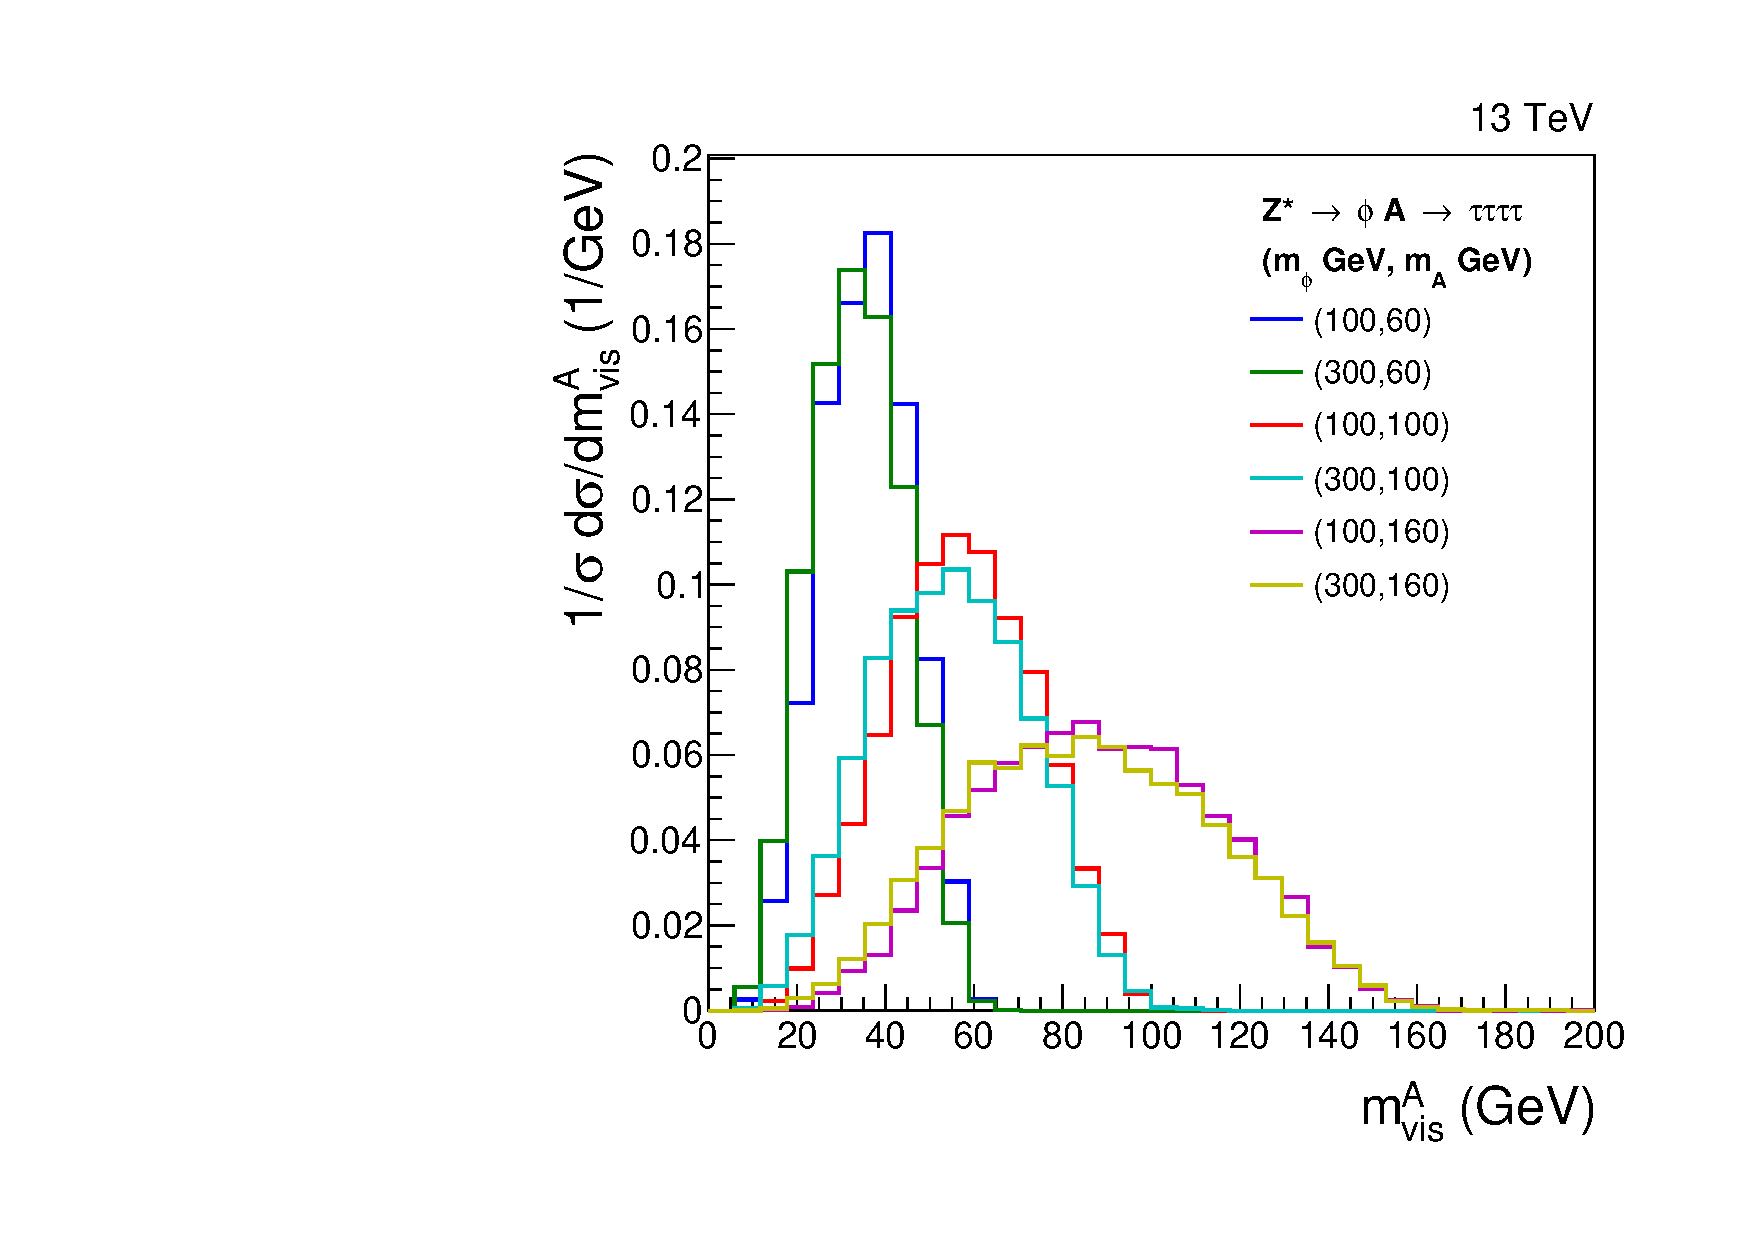
\includegraphics[width=0.49\textwidth]{Figures/mA_dist.pdf}}
    \subfloat[]{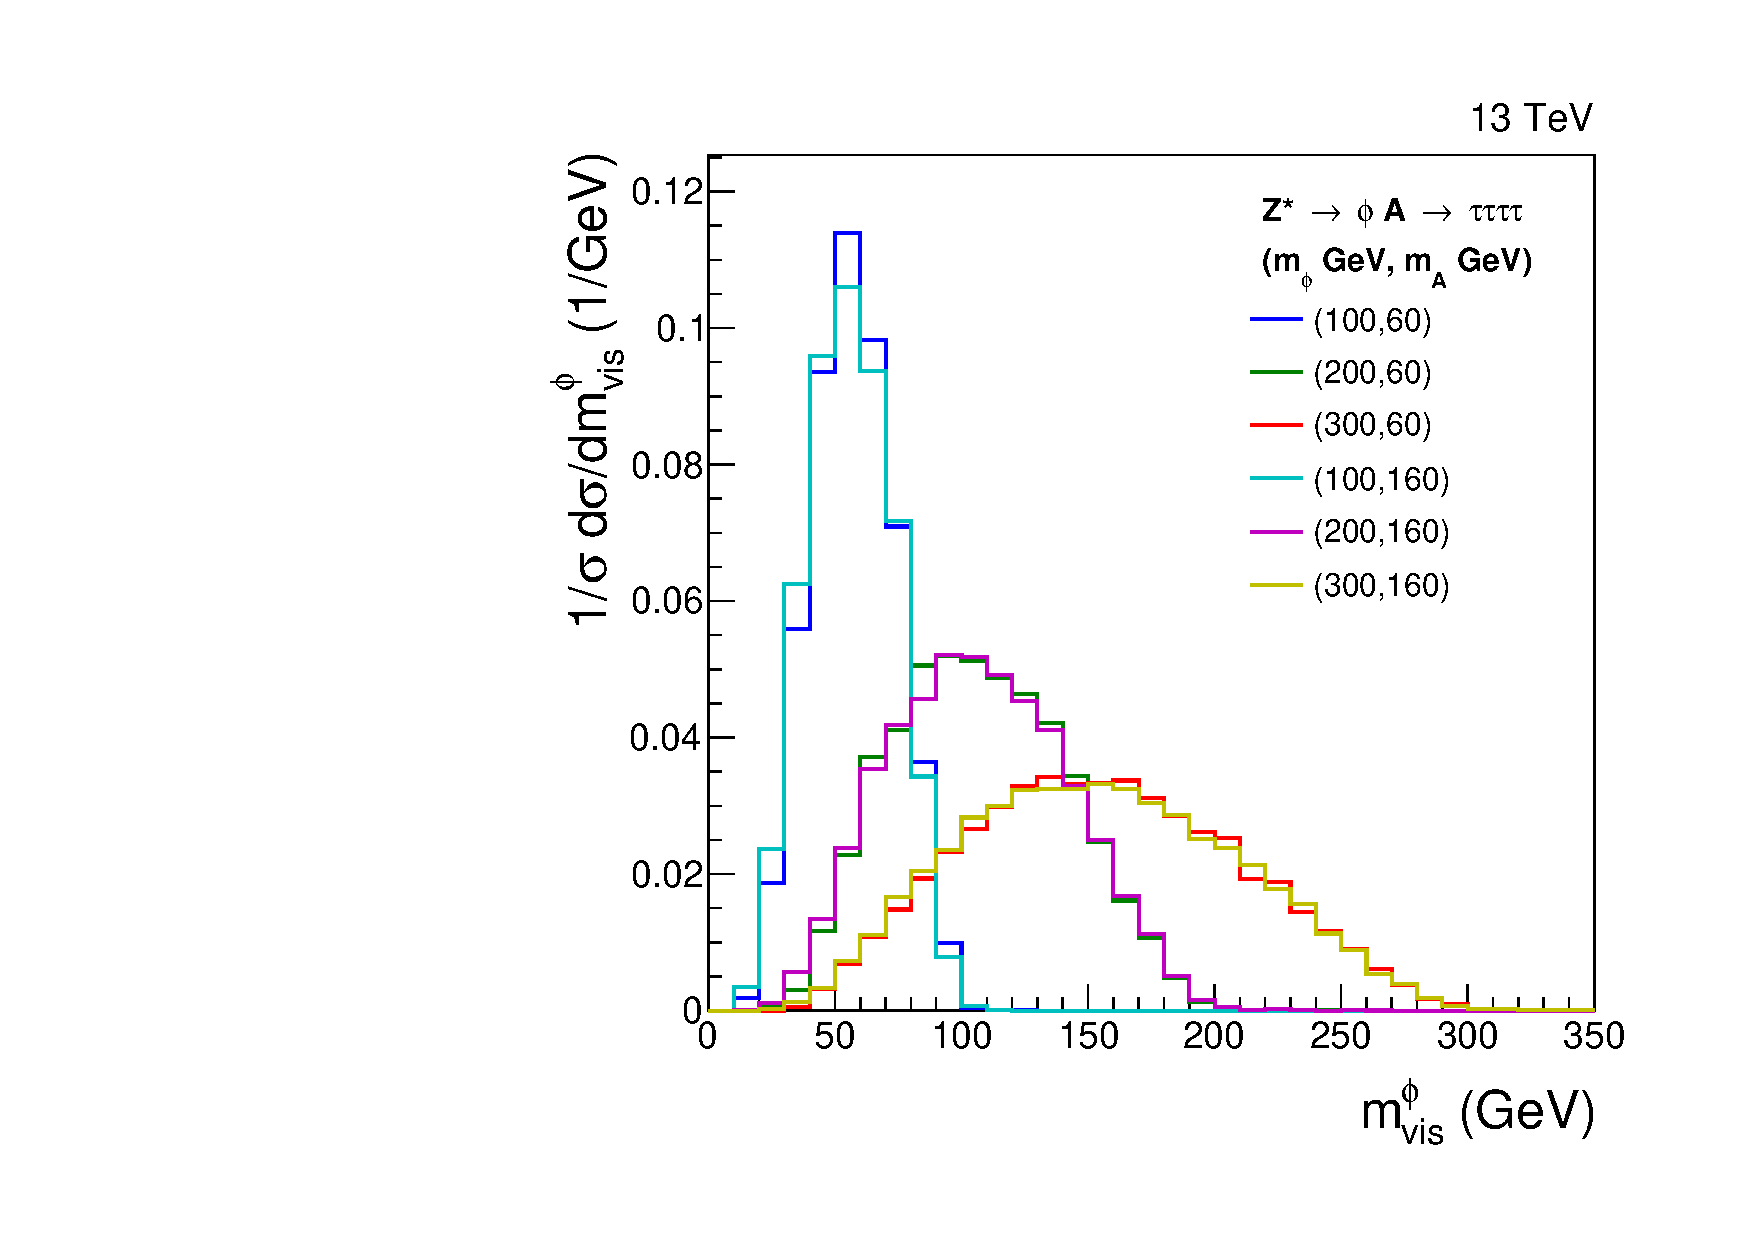
\includegraphics[width=0.49\textwidth]{Figures/mphi_dist.pdf}} 
\caption{Generator level distributions of the visible mass densities for A (a) and $\phi$ (b) for the signal process.}
\label{fig:4tau_gen_dist}
\end{figure}

The cross sections in the alignment scenarios are also determined with this procedure and vary from 10 fb (highest $m_{A}$ and $m_{\phi}$ scenario) to 650 fb (lowest $m_{A}$ and $m_{\phi}$ scenario), as shown in Figure~\ref{fig:4tau_xs}.
These are independent of $\tan\beta$, however, out of the alignment scenarios the cross sections for H scales with $\sin^{2}(\beta-\alpha)$ and h scales with $\cos^{2}(\beta-\alpha)$. \\

\begin{figure}[!hbtp]
\centering
    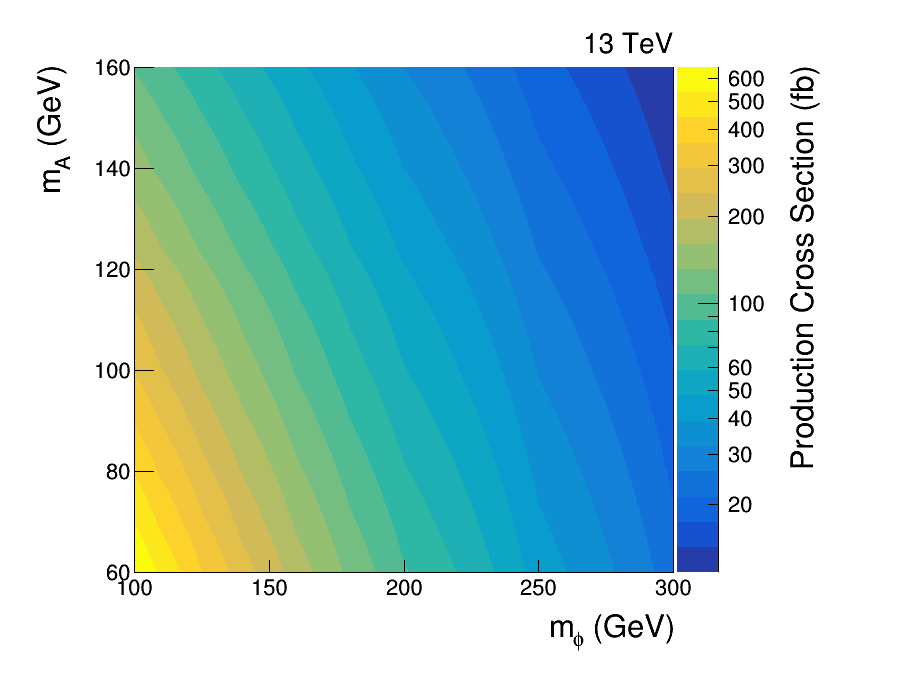
\includegraphics[width=0.8\textwidth]{Figures/cross_sections.png}
\caption{Calculated productions cross sections for the $Z^{*} \rightarrow \phi A$ process, varying the masses of $\phi$ and A.}
\label{fig:4tau_xs}
\end{figure}

The branching fractions of $\phi$ and A to pairs of $\tau$ leptons is dependent on both $tan\beta$ and $\beta-\alpha$.
For this analysis, the branching fractions are calculated using \texttt{2HDECAY} \cite{Krause:2018wmo}.
In the alignment scenarios, the $A\rightarrow\tau\tau$ branching fractions are approximately 1 above $\tan\beta \approx 2$, where below they sharply drop off and other processes such as $A\rightarrow b\bar{b}$ become dominant.
This is also true for $\phi\rightarrow\tau\tau$ branching fractions, except in the case where $m_\phi$ is greater than $m_A$ by more than $m_Z$ and so the $\phi\rightarrow ZA$ decay becomes kinematically feasible and can dominate at high $\tan\beta$.
Examples of this are shown in Figure~\ref{fig:4tau_br_1d}.
Out of the alignment scenario, the branching fractions of $\phi$ to tau leptons becomes smaller as the magnitude of the coupling of additional neutral Higgs bosons to taus is reduced, whilst the $A$ branching fractions, like the couplings, are left unchanged.
An example of the $\phi$ branching fractions out of the alignment scenario is shown in Figure~\ref{fig:4tau_br_2d}.

\begin{figure}[!hbtp]
\centering
    \subfloat[]{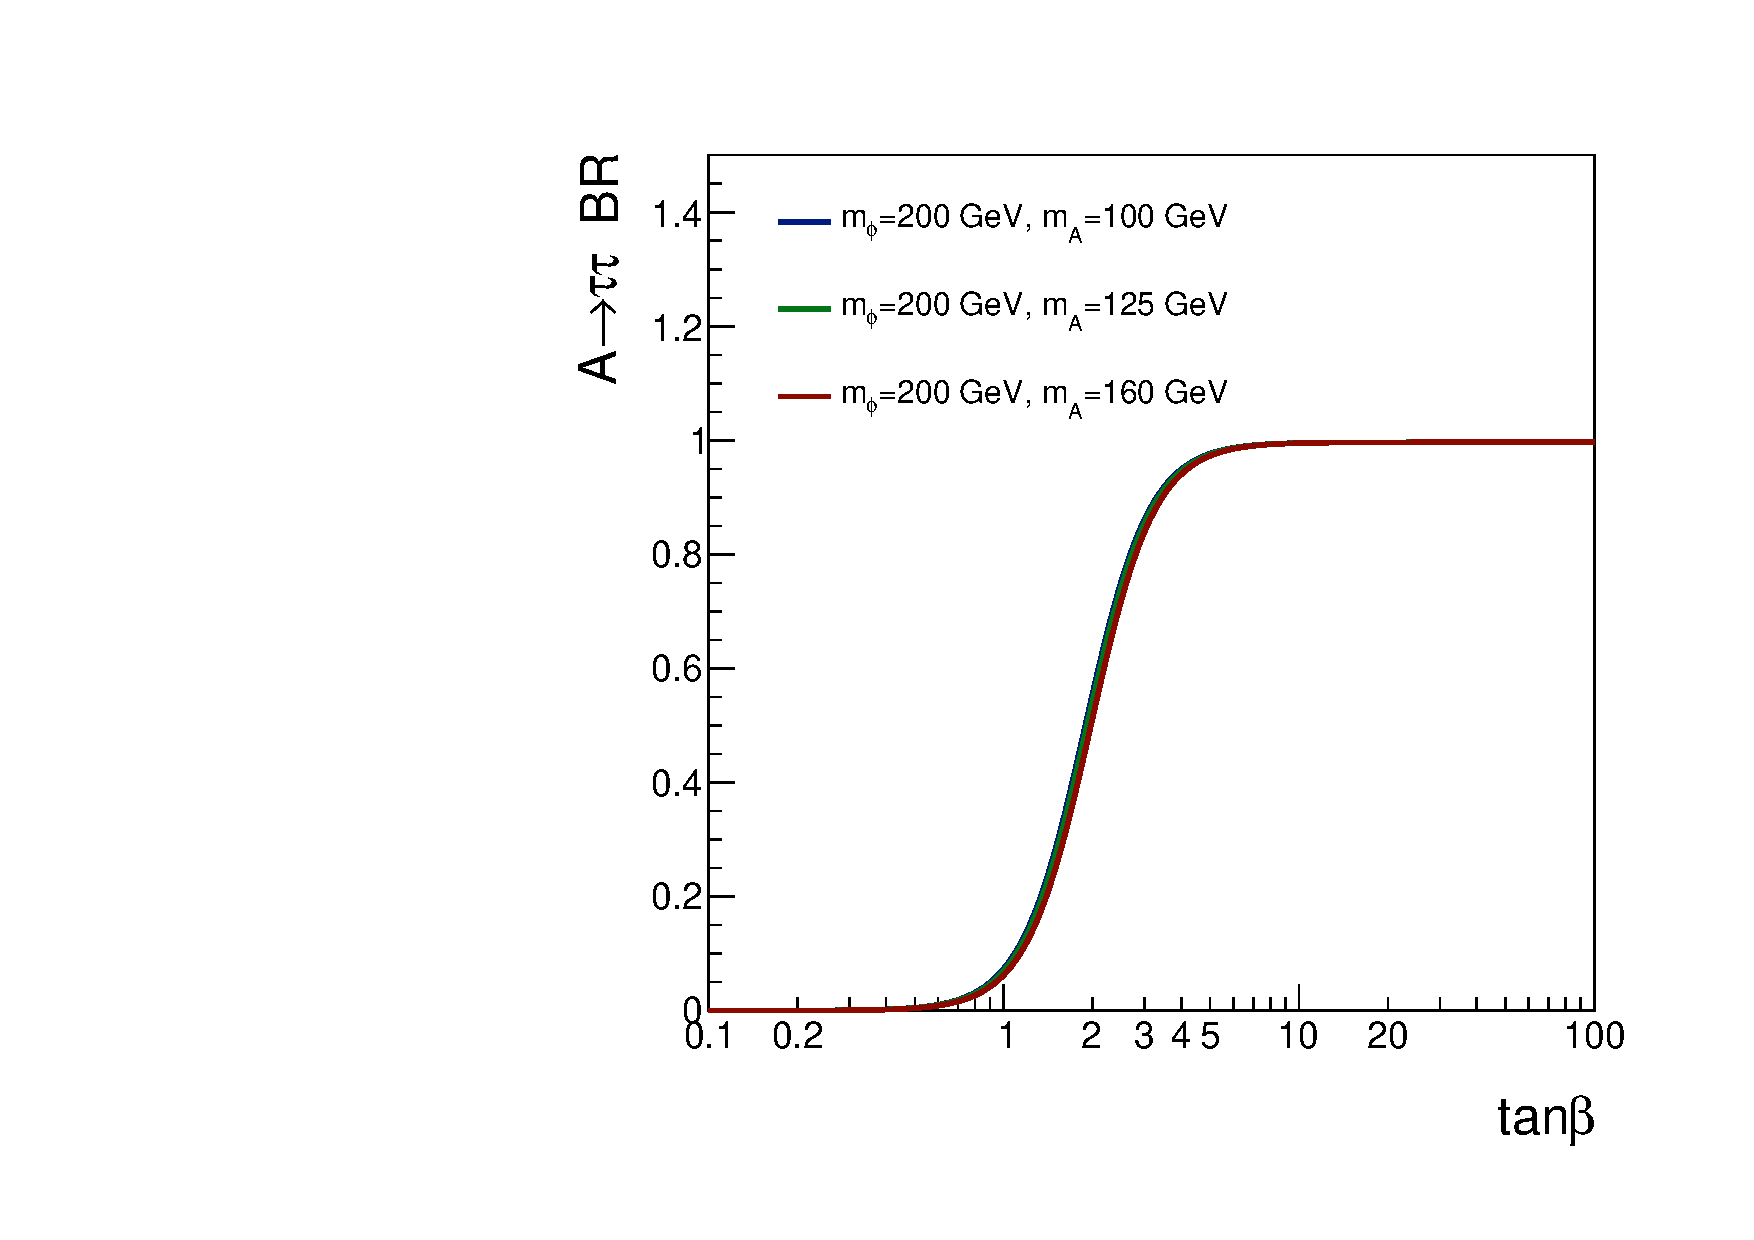
\includegraphics[width=0.49\textwidth]{Figures/A_br_plot_mphi200.pdf}}
    \subfloat[]{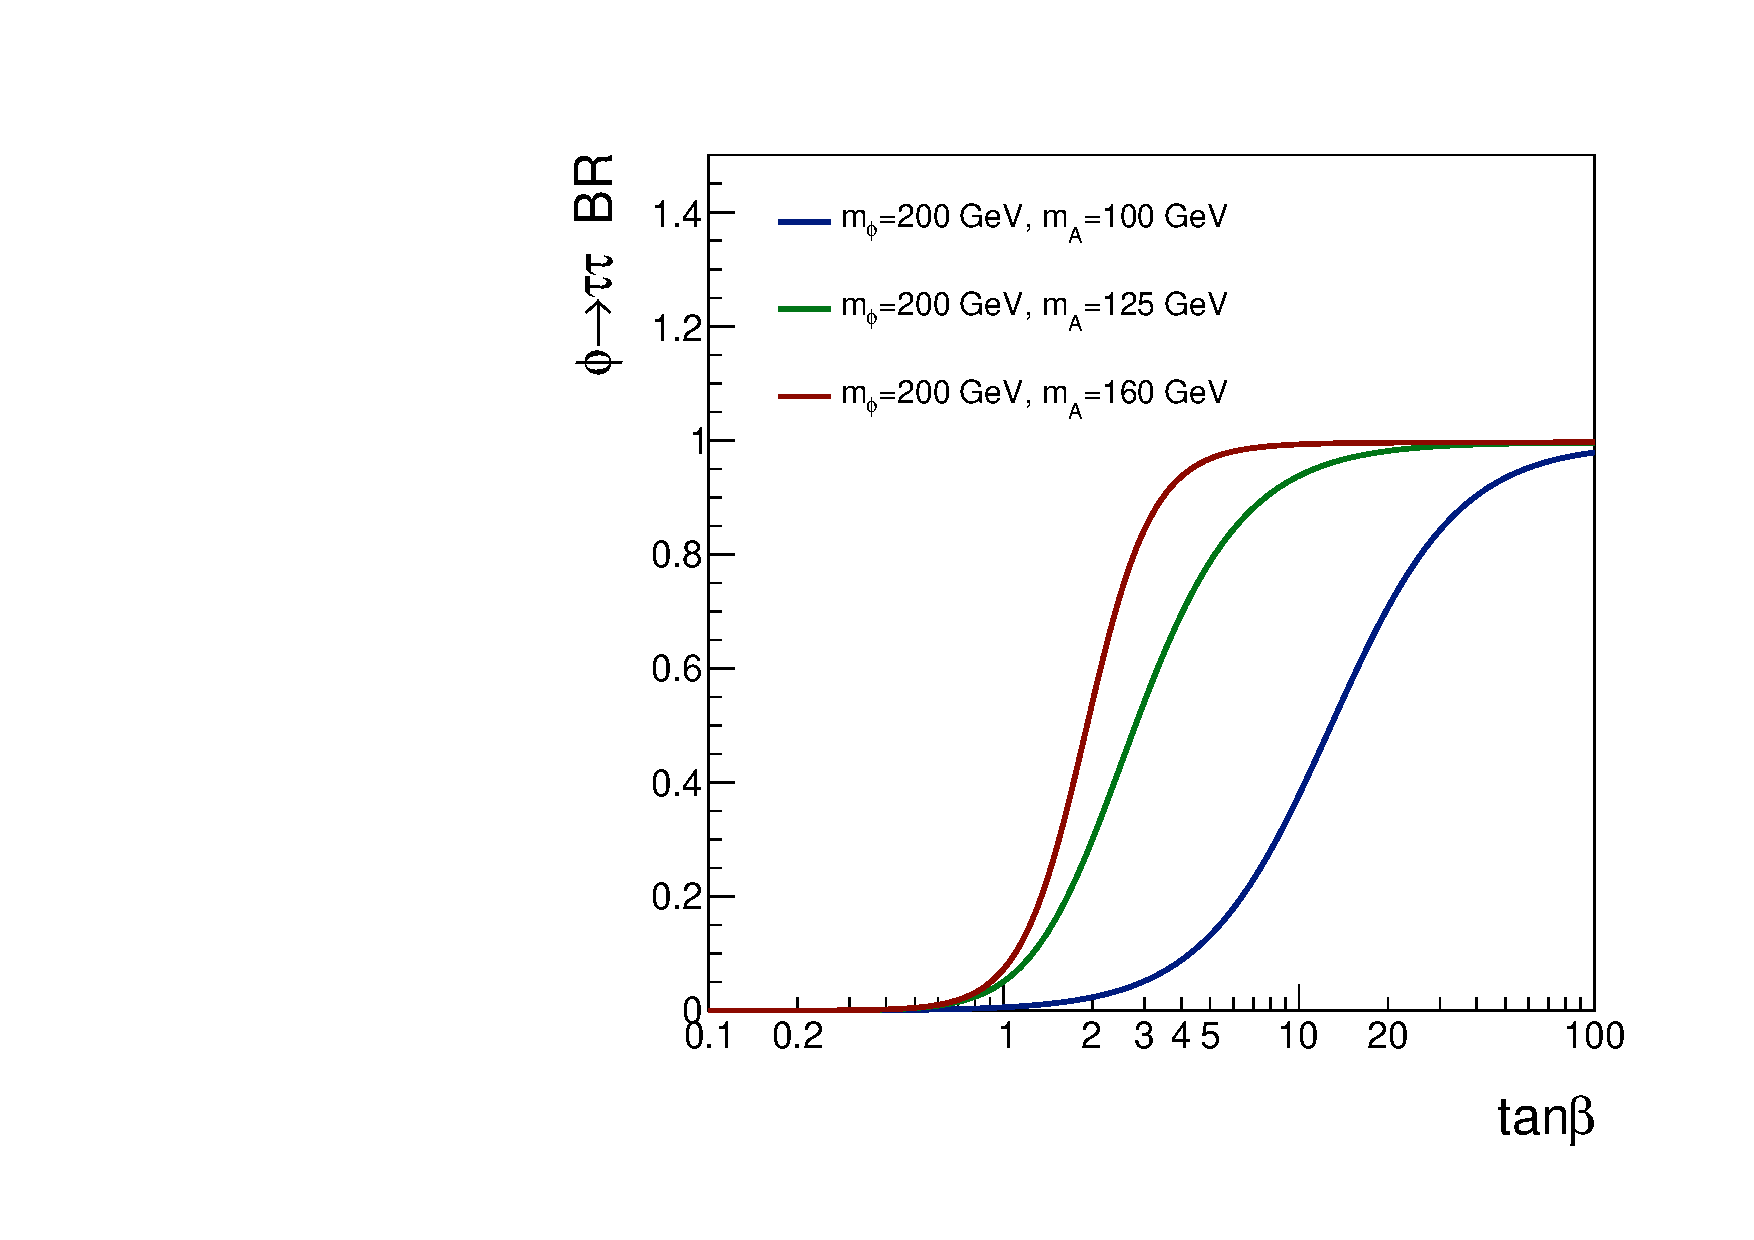
\includegraphics[width=0.49\textwidth]{Figures/phi_br_plot_mphi200.pdf}} 
\caption{Calculated branching fractions of A (a) and $\phi$ (b) decaying to a pair of $\tau$ leptons for various mass scenarios.}
\label{fig:4tau_br_1d}
\end{figure}

\begin{figure}[!hbtp]
\centering
    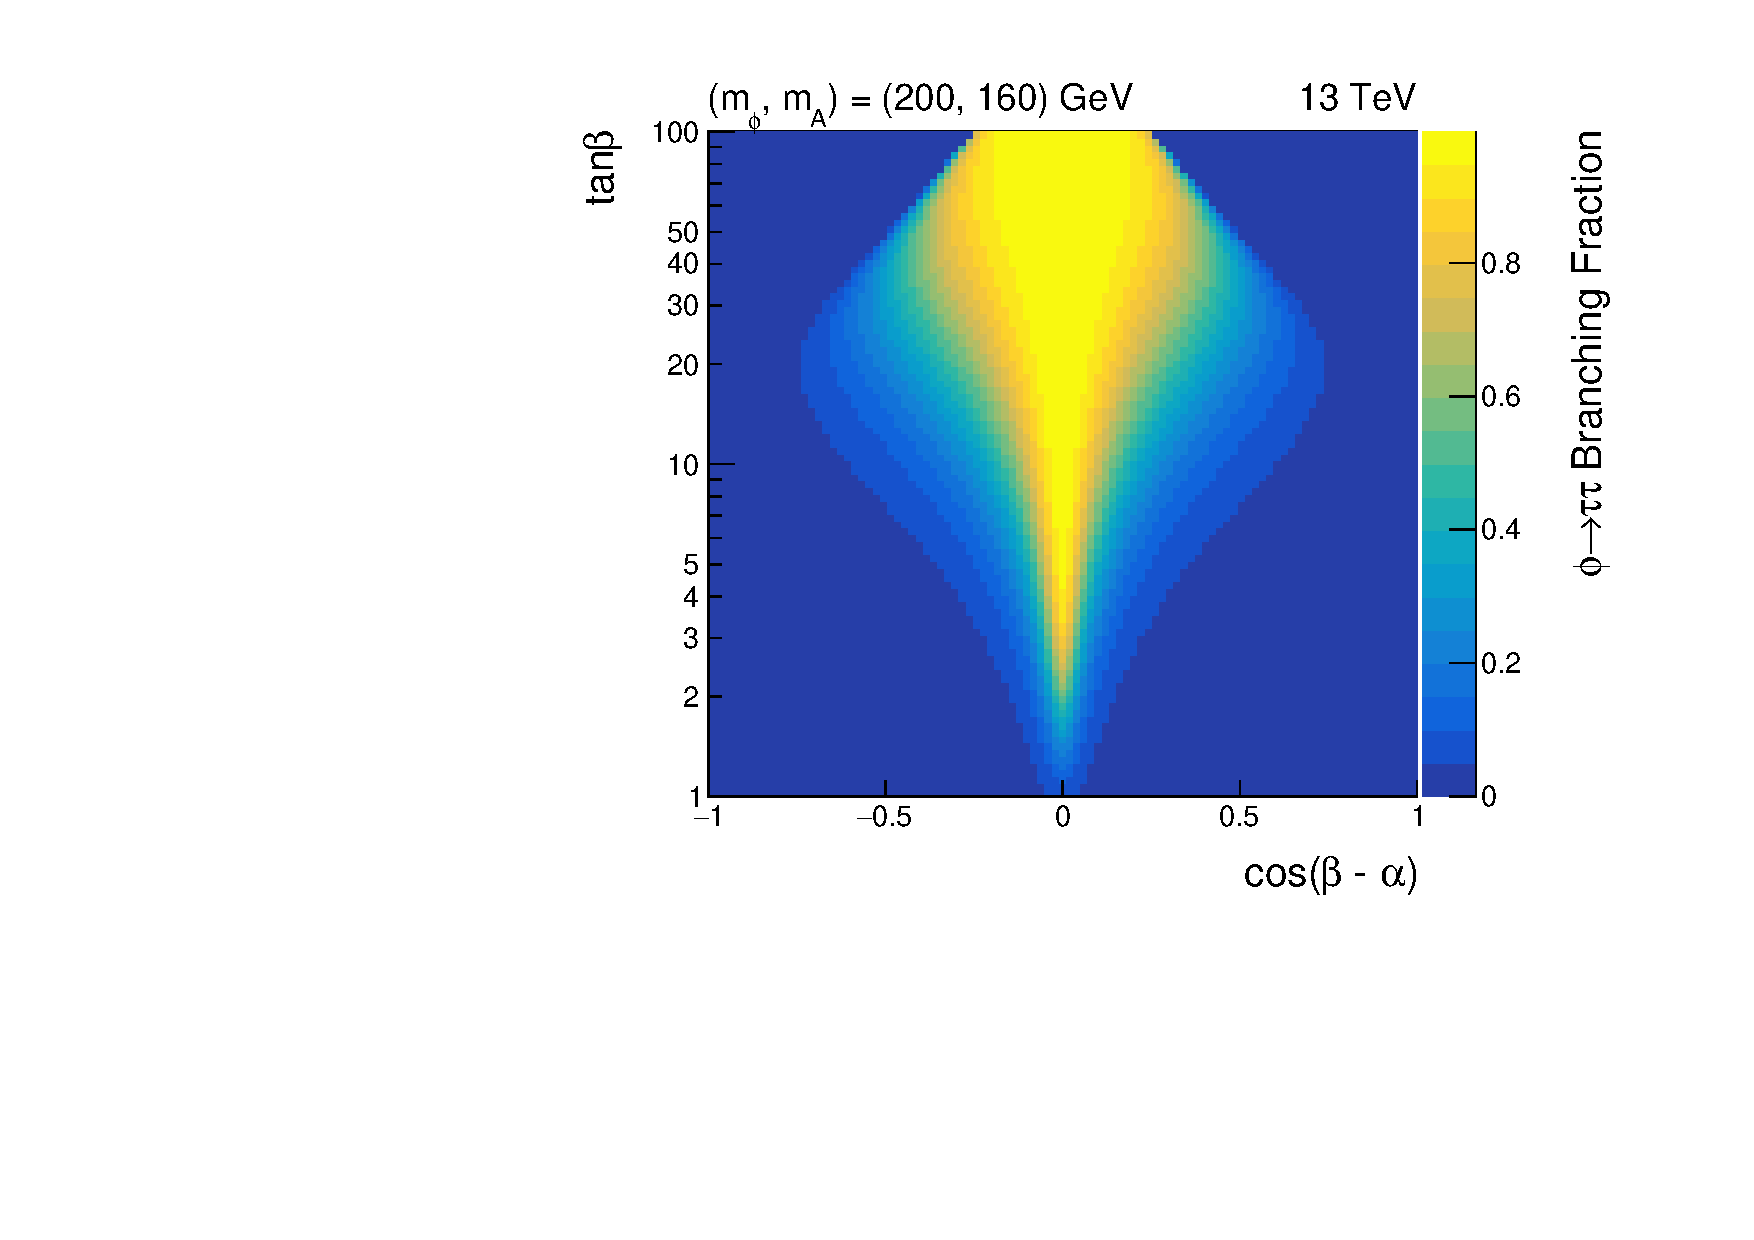
\includegraphics[width=0.7\textwidth]{Figures/phi_branching_fractions_mphi200_mA160.pdf}
\caption{Calculated branching fractions in the $\cos(\beta-\alpha)$-$\tan\beta$ phase space for $\phi$ of mass 200 GeV decaying to a pair of $\tau$ leptons, in the scenario where $m_A = 160$ GeV.}
\label{fig:4tau_br_2d}
\end{figure}

\section{Event Selection}

In comparison to Chapter~\ref{sec:bsm_H_to_tau_tau_analysis}, four $\tau$ leptons produce a much larger number of possible final states. 
All variations of e, $\mu$ and $\tau_h$ final state combinations and their branching fractions are shown in Table~\ref{tab:4tau_bf}.
Just under 90\% of the branching ratio goes to decay products containing two or more hadronic taus.
These are the main final states that are explored in this analysis. 
In addition to this, an orthogonal $\tau_h \tau_h \tau_h$ channel is added to target events where reconstruction of the $\tau_h \tau_h \tau_h \tau_h$ channel loses a single $\tau_h$ object.
This can come about due to low triggering and ID efficiency of $\tau_h$ candidates, as well as the high $\pT$ thresholds required for both. \\
In total, the analysis consists of 7 channels.

\begin{table}[H]
    \centering
    \begin{tabular}{|c|c|}
         \hline
         Channel & Branching Fraction  \\
         \hline
         \hline
         $e \tau_h \tau_h \tau_h$ & 19.4\% \\
         $\mu \tau_h \tau_h \tau_h$ & 18.9\% \\
         $\tau_h \tau_h \tau_h \tau_h$ & 17.6\% \\
         $e \mu \tau_h \tau_h$ & 15.6\% \\
         $e e \tau_h \tau_h$ & 8.0\% \\
         $\mu \mu \tau_h \tau_h$ & 7.6\% \\
         $e e \mu \tau_h$ & 4.3\% \\
         $e \mu \mu \tau_h$ & 4.2\% \\
         $e e e \tau_h$ & 1.5\% \\
         $\mu \mu \mu \tau_h$ & 1.4\% \\
         $e e e \mu$ & 1.4\% \\
         $e e \mu \mu$ & 0.6\% \\
         $e \mu \mu \mu$ & 0.4\% \\
         $e e e e$ & 0.1\% \\
         $\mu \mu \mu \mu$ & 0.1\% \\
         \hline
    \end{tabular}
    \caption{Branching fractions of four $\tau$ leptons, where e and $\mu$ represent the leptonic decay of the $\tau$ and $\tauh$ represent the hadronic decay of the $\tau$.}
    \label{tab:4tau_bf} 
\end{table}

\subsection{Trigger Requirements}

Given that each final state is not exactly triggered on, there is no obvious choice for what triggers to use. 
A variety of triggers are available for individual and clusters of objects in the final state. 
The possible triggers for single objects are the single-e and single-$\mu$ triggers. 
This is not the case for the single-$\tau_h$ trigger as it has a $\pT$ threshold too high for it to be useful. 
The possible triggers for clusters of objects are the double-e, double-$\mu$, double-$\tau_h$, e-$\mu$ cross, $\mu$-$\tau_h$ cross and e-$\tau_h$ cross-triggers.
The cross-triggers and double-e/$\mu$ triggers are found to offer little improvement to the signal acceptance and so these events are not included.
Any combination of objects in the final state of a channel can be selected by these triggers and the union of events passing each iteration is taken. 
The trigger $\pT$ and $\eta$ thresholds for the remaining triggers (single-e/$\mu$ and double-$\tauh$) are equivalent to what is stated in Section~\ref{sec:trig_ditau}.

\subsection{Offline Requirements}

All offline selections stated are in addition the object selection discussed in Section~\ref{sec:object_reconstruction}.
In this analysis, $\tau_h$ candidates are required to pass the \texttt{Loose} $D_{\text{jet}}^{\text{WP}}$.
The \texttt{VVLoose} $D_{e}^{\text{WP}}$ and \texttt{VLoose} $D_{\mu}^{\text{WP}}$ are used in all decay channels.
These working points are chosen to maximise the sensitivity of the analysis and looser cuts are used than in Chapter~\ref{sec:additional_higgs_bosons} to ensure there are enough statistics to account for the stricter selection of more objects in the final states. \\

On top of the object selection, there are few further selections on the total tau collection.
As the two tau pairs from the signals originate from two neutral additional Higgs bosons, the sum of charge of the fully reconstructed objects should be 0. 
This is applied in the decay channels where there are four objects. 
In the $\tau_h \tau_h \tau_h$ channel, as the assumption is that a hadronic tau has been lost, the absolute value of the sum of the charges of the object is required to be 1.
In order to ensure the orthogonality between channels, a number of vetos are needed. 
Firstly, extra lepton vetos are used in all decay channels, where the absence of additional electrons and muons in required on top of those already part of the selected pair.
The kinematic requirements, ID and isolation requirements on these extra leptons are at least as loose as the loosest cuts required for signal electron or muon of the final states.
Secondly, an extra $\tau_h$ veto is applied to the $\tau_h \tau_h \tau_h$ channel, in order to keep it orthogonal to the $\tau_h \tau_h \tau_h \tau_h$ channel.
Here any extra $\tau_h$ candidate passing the signal selection is vetoed
The constraints set on the number of leptons and $\tau_h$ candidates for each channel are shown in Table~\ref{tab:leptonvetoes}. \\

\begin{table}[H]
   \centering
   \begin{tabular}{|l|c|c|c|}
   \hline
   \multicolumn{1}{|c|}{Channel} & e & $\mu$ & $\tau_h$ \\ \hline \hline
   $\tau_h \tau_h \tau_h \tau_h$ & 0 & 0     & $\geq$4        \\
   $\tau_h \tau_h \tau_h$        & 0 & 0     & 3        \\ 
   $\mu \tau_h \tau_h \tau_h$    & 0 & 1     & $\geq$3        \\
   $e \tau_h \tau_h \tau_h$      & 1 & 0     & $\geq$3        \\
   $e \mu \tau_h \tau_h$         & 1 & 1     & $\geq$2        \\
   $\mu \mu \tau_h \tau_h$       & 0 & 2     & $\geq$2        \\
   $e e \tau_h \tau_h$           & 2 & 0     & $\geq$2        \\ \hline
   \end{tabular}
   \caption{Vetoes set on the number of leptons for each channel.}
   \label{tab:leptonvetoes}
\end{table}

Finally, in channels containing an electron or a muon, a veto on events with one or more b tagged jets is placed.
This is done to remove the $\ttbar$ background process in a region where little to no signal is expected.
This is not done in the fully $\tau_h$ channels as the $\ttbar$ process is negligible. \\

\section{Search Optimisation}

Due to the limited statistics in each decay channel, only minimal categorisation of events can be performed and the only divisions of the decay channels happen in final states with two light leptons and two $\tau_h$ candidates, where two categories are made.
These separate events where the light leptons have the same charge (\texttt{SS Leptons}) and where they have opposite charge (\texttt{OS Leptons}).
This is motivated to separate regions where specific background processes are dominant.
In particular, a large portion of the $ee\tauh\tauh$ and $\mu\mu\tauh\tauh$ channel backgrounds come from $Z\rightarrow ll$ (or $Z\rightarrow\tau\tau\rightarrow ll$) with 2 jets misidentified as $\tauh$ candidates, where the two light leptons are of opposite sign.
Similarly, the $e\mu\tauh\tauh$ channel contains more background events with an opposite sign electron and muon, from a Z decay via taus or from the $\ttbar$ process.
There is no preference for light lepton charge sums in the signal samples and so more sensitivity to the signal is expected in the \texttt{SS Lepton} categories. 
A summary of the categorisation and b tag selection is shown in Figure~\ref{fig:4tau_categories}. \\

\begin{figure}[!hbtp]
\centering
    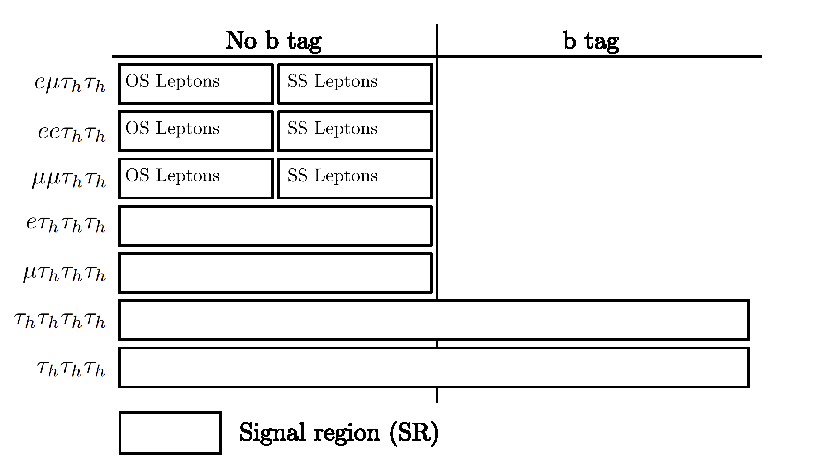
\includegraphics[width=0.85\textwidth]{Figures/event-categories_4tau.pdf}
\caption{Overview of the categories used for the extraction of the signal in the $Z^{*}\rightarrow \phi A \rightarrow 4\tau$.}
\label{fig:4tau_categories}
\end{figure}

Similarly to Chapter~\ref{sec:additional_higgs_bosons}, events in each 10 analysis channels and categories are drawn out into histogram based off the same discriminating variable, the total transverse mass ($m_{T}^{\text{tot
}}$).
However, as there are more objects in the final state, the definition is extended to what is shown below.
\begin{equation}
m_{T}^{\text{tot}} = \sqrt{ \sum_{i=1}^{N_\tau} m_{T}(\vec{p}_{T}^{\hspace{2pt}\tau_i},\vec{p}_{T}^{\hspace{2pt}\text{miss}})^2 + \sum_{i,j=1; i \neq j}^{N_\tau} m_{T}(\vec{p}_{T}^{\hspace{2pt}\tau_i},\vec{p}_{T}^{\hspace{2pt}\tau_j})^2 },  
\end{equation}
where $N_\tau$ is the number of objects in the final state, and $\tau_i$ refers to the visible products of the i'th $\tau$ lepton.
This variable again provides excellent discriminating power between resonant signals compared to other non-peaking backgrounds, whilst still maintaining some separation between signal masses.
The sensitivity of this discriminating variable was tested against many others, including the visible masses of the two bosons which can be separated to $\approx 90\%$ efficiency after selection into the correct pairs. 
As $m_{T}^{\text{tot}}$ uses information about the whole event, in particular the higher $p_{T}$ objects and high MET from many $\tau$ decays, a greater sensitivity to the signal is observed. \\

In this analysis, many of the histograms contain very few background events and in order to minimise statistical fluctuations in the background templates, histogram bins are merged based off the fractional statistical uncertainty of each bin.
This leads to a number of single and minimally binned channels/categories where background statistics are low but signal sensitivity is high and a few finely binned and high statistic channels/categories able to better classify the signal, if one is observed.
 
\section{Background Modelling Overview}

The backgrounds are split into a three categories:
\begin{enumerate}[i)]
  \item Events containing only genuine $\tau$ leptons.
  \item Events with one or more jet misidentified as a $\tau_h$ (jet$\rightarrow \tauh$).
  \item Events where all $\tauh$ candidates are either correctly identified or a misidentified light lepton. 
\end{enumerate}

Background contributions from (i) are mostly from gluon and quark initiated di-Z production and is modelled using MC.
The details and validation of this modelling is described in Section~\ref{sec:zz_modelling}.
Background (ii) accounts for a number a different process with jets misidentified as a $\tau_h$ candidate.
Examples of this are single-Z, single-W and $\ttbar$ productions with additional jets in the events being misidentified.
This is modelled with a fake factor method, similar to what is described in Section~\ref{sec:ff}, but using machine learning to improve upon method, and discussed further in Section~\ref{sec:ml_ff}.
The latter contribution is very small in comparison to the others and modelled with MC.
Events with jets misidentified as light leptons and no jets misidentified as $\tauh$ candidates have been checked with MC and deemed negligible in all channels. \\

All MC background samples described in Section~\ref{sec:background_modelling} are modelled in the same manner.  
In addition, tri-boson samples are used that are generated using \MGvATNLO at next-to-LO (NLO) precision~\cite{Alwall:2011uj}.
All corrections described in Section~\ref{sec:ditau_corrections} are applied to MC, with extra corrections are applied on the ZZ$\rightarrow$4l process, that are detailed in Section~\ref{sec:zz_modelling}.

\section{ZZ Modelling}
\label{sec:zz_modelling}

The di-Z background shapes are modelled using MC.
The cross-sections for this analysis are scaled to high order precisions than the signal generation using k factors.
For quark initiated di-Z production, \POWHEG~\cite{} is used to determine NNLO/NLO QCD and EW corrections as a function of $m_{ZZ}$, which takes an average value of $\approx 1.2$.
Gluon initiated di-Z production corrections from LO to NNLO is derived with HNNLO v2~\cite{}, again as a function of $m_{ZZ}$.
This gives a much larger correction, equal to $\approx 2$.
The modelling is validation using a $\mu\mu\mu\mu$ final state and good agreement is observed between data and simulation.
Identical object selection is applied as stated in Section~\ref{sec:object_reconstruction}, except to ensure better statistics within the channel, the $I_{\text{rel}}^{\mu}$ cut is loosened to 0.35.
The charges of the $\mu$ candidates are similarly required to sum to one and no vetos on the number of b jets in the event is applied.
Plots of this are shown in Figures~\ref{fig:4tau_mmmm}. \\

\begin{figure}[!hbtp]
\centering
    \subfloat[]{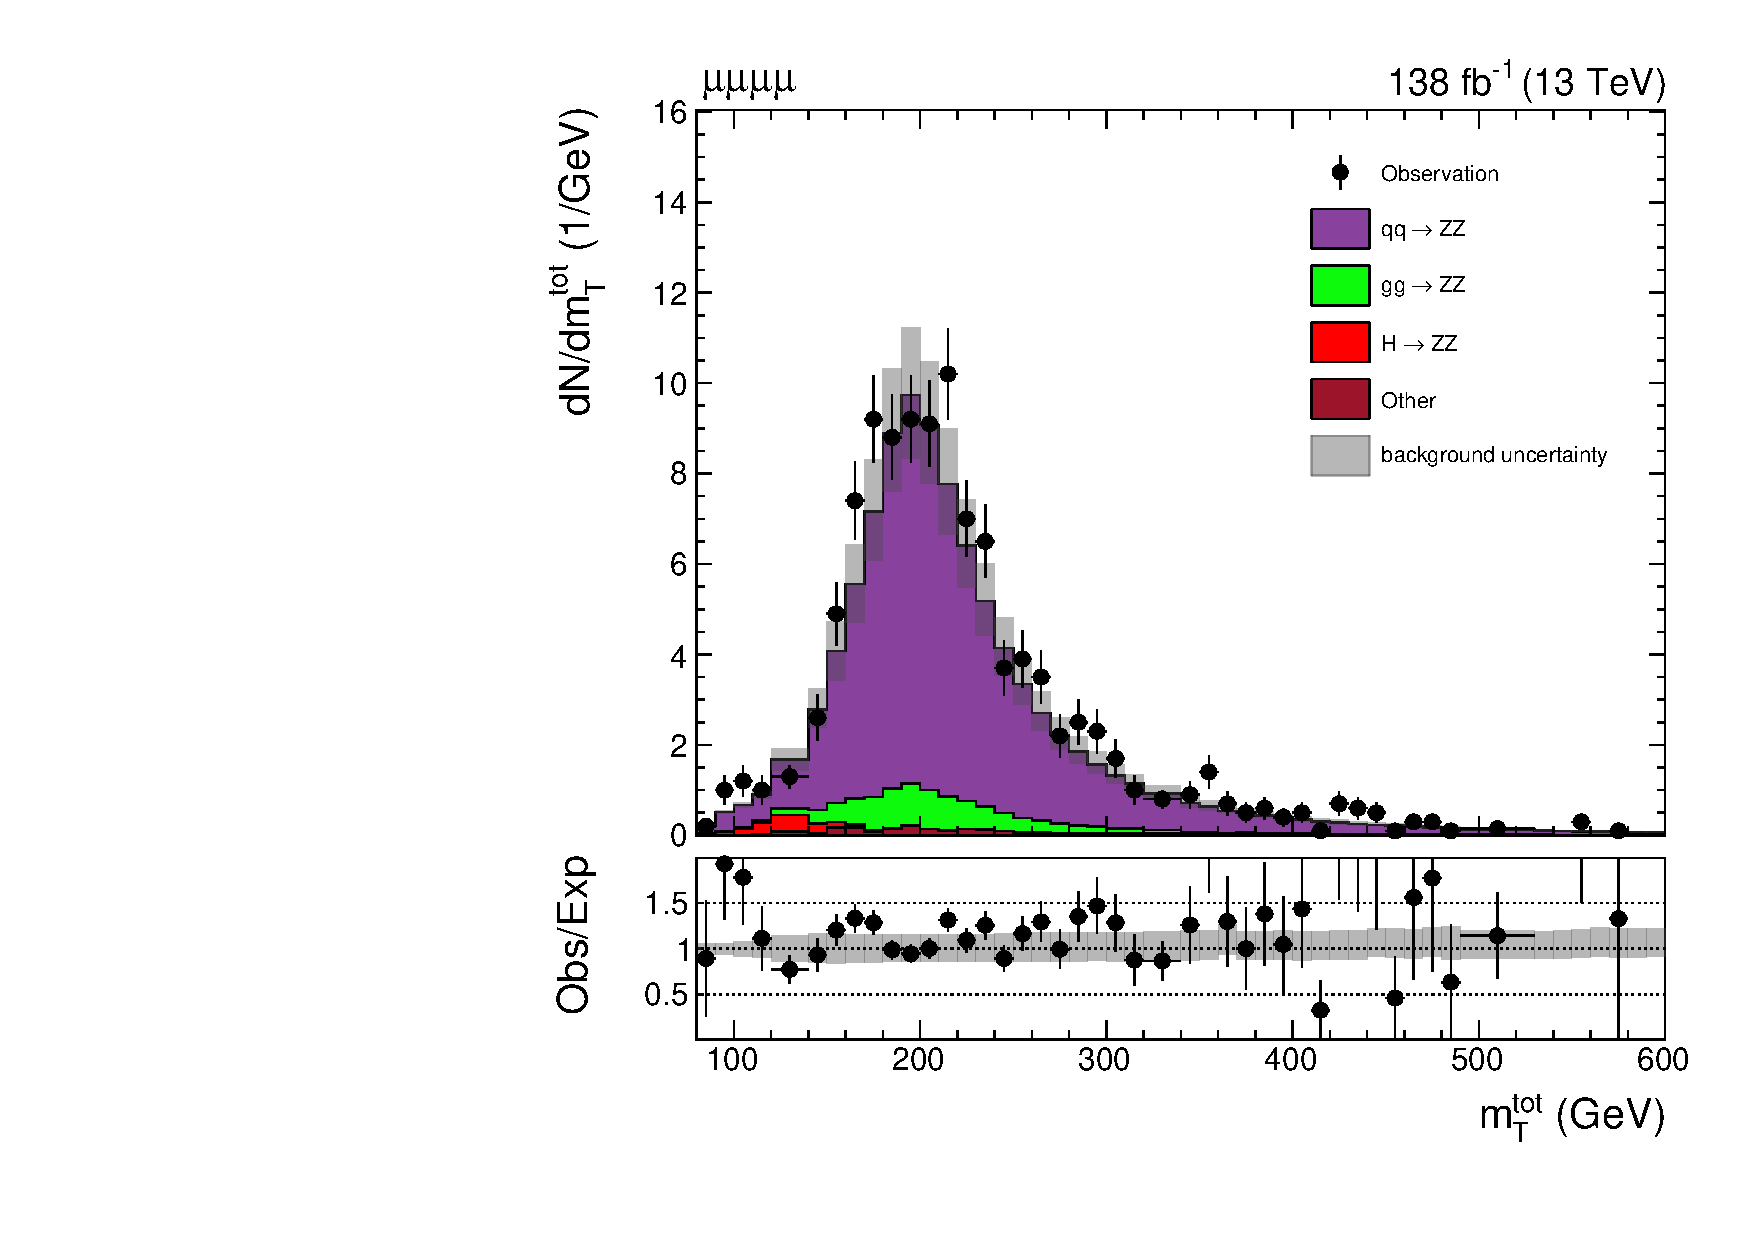
\includegraphics[width=0.49\textwidth]{Figures/mt_tot_signal_mmmm_inclusive_all.pdf}}
    \subfloat[]{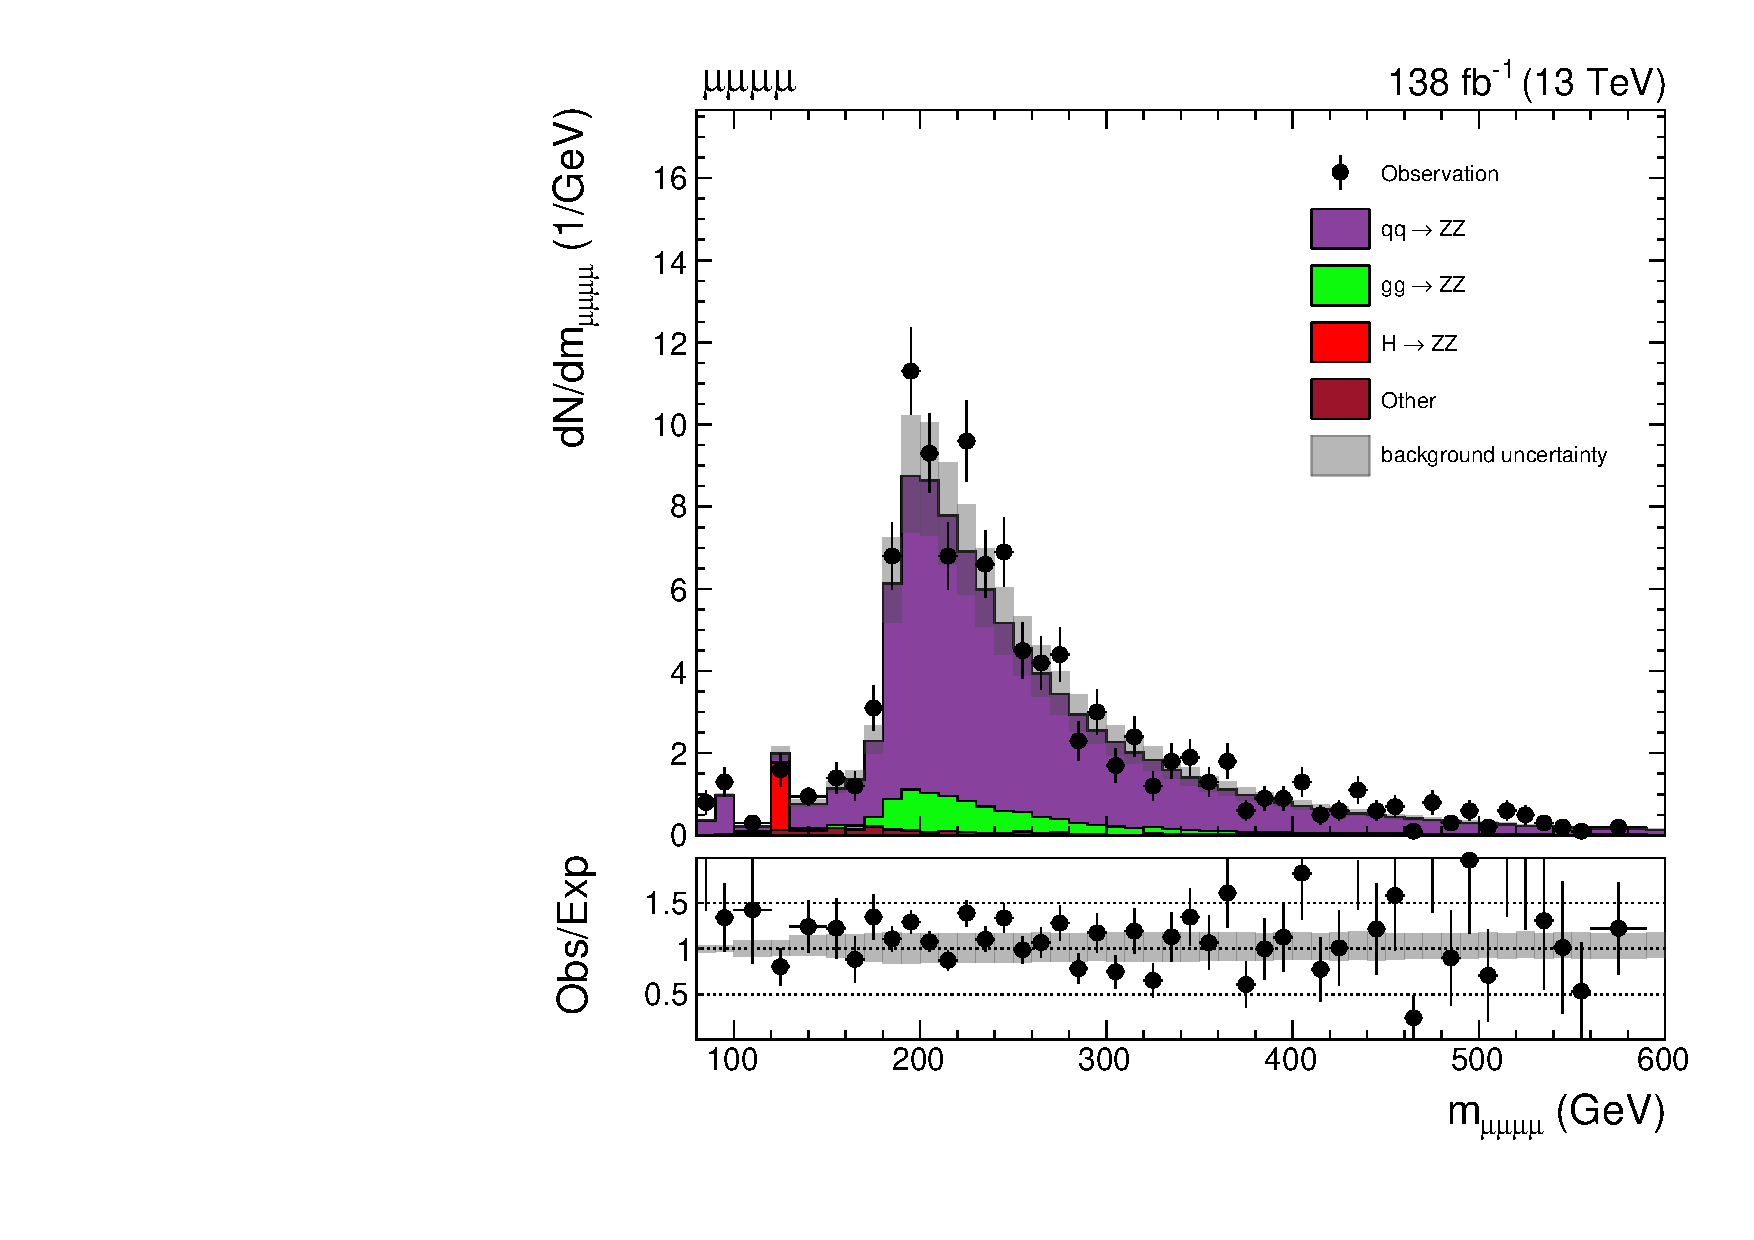
\includegraphics[width=0.49\textwidth]{Figures/mvis_1234_signal_mmmm_inclusive_all.pdf}} 
\caption{Distributions in the $\mu\mu\mu\mu$ channel are shown for the variables total transverse mass, $m_{T}^{\text{tot}}$, (a) and the total mass, $m_{\mu\mu\mu\mu}$ (b). The solid histograms show the stacked background predictions.}
\label{fig:4tau_mmmm}
\end{figure}


\section{Machine Learning Fake Factor Method}
\label{sec:ml_ff}

The fake factor method, as described in Section~\ref{sec:ff}, is an algorithm used to model the jet$\rightarrow \tauh$ backgrounds.
It uses classical reweighting techniques, such as binning the two regions and applying a fit to the ratio in a chosen parametrisation.
This method faces difficulties when approached with highly dimensional dependence on the parametrisation.
In this scenario, classical "bin and fit" methods can break down, as for every new parameter included the statistics of each fit is reduced.
A compromise must then be reached between variable dependence and fit statistics and is the case for the jet-$\pT$/$\tauh$-$\pT$ binning described in Section~\ref{sec:ff_params}.
It is also the case, that the analysis in Section~\ref{sec:additional_higgs_bosons} uses well checked assumptions on for example, the consistency of $\tauh$ decay modes from determination to signal regions, in order to average across the dependencies on this variable when calculating fake factors, however this will not always be the case.
Also binned upon in the previous search, is the process dependence of the fake factors.
The binning used is an admission that the relevant parametrisation of the fake factors between process is too complication to model with "bin and fit" methods.
It can also be seen that the initial fits, do not do a good job at modelling all variables as corrections are needed. \\

There is final problem with using a fake factor method as described, when there are multiple $\tauh$ candidates in final states. 
In the $\tauh\tauh$ channel of the previous analysis, the fake factors were only calculated from the leading-$\tauh$ candidate.
This was valid, as the dominant backgrounds had two jet $\rightarrow\tauh$ candidates rather than one genuine $\tauh$ and one jet$\rightarrow\tauh$ candidate.
However, for this search this assumption is not valid. \\

All of these reason motivate a more generalised and smarter method to model jet $\rightarrow\tauh$ backgrounds, as well as the extra importance on modelling these backgrounds where there are more $\tauh$ candidates in the final state.
This is done utilising machine learning and in particular using a BDT for the purpose of multi-dimensional reweighting. \\ 

\subsection{BDT Reweighter}

Ref.~\cite{Rogozhnikov:2016bdp} proposes a new method utilising machine learning techniques to solve the issues with dimensionality. 
It looks to optimise the regions that most need reweighting. 
One good way to do this is using a decision tree, as with this the data can be split into "leafs" by checking simple conditions.
To best choose the regions that need reweighting the algorithm looks to maximise the symmetrised $\chi^2$.

\begin{equation}
\chi^2 = \sum_{\text{leaf}} \frac{(w_{\text{leaf, 1}}-w_{\text{leaf, 2}})^2}{(w_{\text{leaf, 1}}+w_{\text{leaf, 2}})^2}
\end{equation}

The larger the value of $\chi^2$ the more important reweighting is in this region. 
The kind of tree is utilised many times in the reweighting algorithm shown below:

\begin{enumerate}[i)]
\item Input training dataset with a large number of variables.
\item Build a tree as stated above. If not the first loop, use newly determined weights.
\item Compute predictions in the leaves $r_{\text{leaf}} = \log\frac{w_{\text{leaf, 1}}}{w_{\text{leaf, 2}}}$. The logarithm is taken so weights in different trees can be summed as usually done in boosting.
\item In each leaf MC events by $w = w \times e^{r_{\text{leaf}}}$.
\end{enumerate}

The final two steps are identical to the first approach except for the use of the logarithm for convenience using boosting. 
The major difference being how the bins used for reweighting are found, and that this step is repeated multiple times. \\

\subsection{Fitting Regions}

Unlike the standard fake factor method, statistics are not a problem using the BDT reweighter when choosing which variables you can use to parametrise the fake factors. 
Therefore, rather than fitting two fake factor regions separately and then a correction from sideband to signal to account for missing parametrisation, regions A,B and D from Figure~\ref{fig:ff_schematic} are fit simultaneously to improve statistics. 
Also, all $\tauh$ candidates are fit simultaneously as separate entries in the dataset and for each $\tauh$ in the event, the remaining $\tauh$ candidates are named the alternative $\tauh$ candidates, rather than the $\tauh$ that is being fit. 
The sideband variable definitions and cuts, with respect to Figure~\ref{fig:ff_schematic}, are shown below. \\

\begin{enumerate}[i)]
   \item $ee\tauh\tauh$, $e\mu\tauh\tauh$, $\mu\mu\tauh\tauh$, $e\tauh\tauh\tauh$ and $\mu\tauh\tauh\tauh$  \\
     \indent $y_C$: The sum of $\tauh$ candidates is required to be 0. \\
     \indent $y_A$: The sum of $\tauh$ candidates is required to not be 0. \\
     \indent $x_C$: All alternative $\tau_h$ candidates pass the \texttt{Loose} $D_{\text{jet}}^{\text{WP}}$. \\
     \indent $x_D$: At least one alternative $\tau_h$ candidate fails the \texttt{Loose} $D_{\text{jet}}^{\text{WP}}$ but has $D_{\text{jet}}^{\text{score}} > 0.1$.
  \item $\tauh\tauh\tauh$ \\
     \indent $y_C$: The absolute value of sum of $\tauh$ candidates is required to be 1. \\
     \indent $y_A$: The absolute value of the sum of $\tauh$ candidates is required to not be 1. \\
     \indent $x_C$: All alternative $\tau_h$ candidates pass the \texttt{Loose} $D_{\text{jet}}^{\text{WP}}$. \\
     \indent $x_D$: At least one alternative $\tau_h$ candidate fails the \texttt{Loose} $D_{\text{jet}}^{\text{WP}}$ but has $D_{\text{jet}}^{\text{score}} > 0.1$.
\end{enumerate}

These selections mimic what is done for the $\tauhtauh$ channel fake factors from Section~\ref{sec:ff_dr}, where the definitions of the alternative sideband variable are extended to more than one other $\tauh$ candidate.
The $D_{\text{jet}}^{\text{score}} > 0.1$ selection is used as the alternative tau ID selection for this analysis and is also then extended to the alternative $\tauh$ candidates for this selection.
A cut on the score is used instead of a working point as the loosest defined working point does not provide enough statistics to ensure a good fit. \\

Extrapolating the regions used for fitting to the $\tau_h \tau_h \tau_h \tau_h$ channel, there would be some overlap in the fitting region with the $\tau_h \tau_h \tau_h$ signal region. 
As this region is expected to be sensitive to signal, this is not used to model jet $\rightarrow\tauh$ backgrounds in the $\tau_h \tau_h \tau_h \tau_h$ channel. 
Instead the fit from the $\tau_h \tau_h \tau_h$ channel is used. 
There are a few variables that are defined differently in the fit between the two channels due to the difference of four to three objects selected, therefore when getting fake factors in the $\tau_h \tau_h \tau_h \tau_h$, the lowest $D_{\text{jet}}^{\text{score}}$ unused $\tauh$ candidate is dropped and variables recalculated. 
This candidate is chosen to be removed to best mimic the initial selection of the $\tauh$ candidates where they are sorted by $D_{\text{jet}}^{\text{score}}$ and the high scoring candidates are chosen. 
As shown later in this section, there is no major dependence on the shifted variables and any effect from this removal is covered within the uncertainty model. \\

\subsection{Variables Used}

The variables used are variables that have been shown to have fake factor dependence previously CITE SOME STUFF. 
Also added are the variables that take you from A to C and D to C, from Figure~\ref{fig:ff_diagram}. 
As all years are fit together, in order to account for any differences in fake fake factor from year to year, this is also added. 
The final variable added is the $\pT$ ordered ranking of the $\tauh$ candidates in the event.
All these variables are shown below.

\begin{itemize}
\item The HPS decay mode of the hadronic tau candidate.
\item $\pT$ of the hadronic tau candidate.
\item The ratio of the $\pT$  of the matched jet to the $\pT$ of the hadronic tau candidate.
\item $\eta$ of the hadronic tau candidate.
\item The charge of the hadronic tau candidate.
\item A boolean of whether the hadronic tau candidate passes a leg of the double tau trigger.
\item The total charge of the combined objects.
\item The booleon of whether $D_{\text{jet}}^{\text{WP}}$ passes to $\texttt{Loose}$ WP for the other hadronic tau candidates. These are sorted by $\pT$.
\item Year of data taking.
\item $\tauh$ $\pT$ ordered event rank.
\end{itemize}

\subsection{Machine Learning Subtraction Method}

In the standard fake factor method, histograms are used to fit the fake factors rather than datasets. 
Using histograms, the small fraction of events which are not jet fakes can easily be subtracted off. 
To do this, the data histogram is subtracted from by a stacked MC background produced with generator matching ensuring the event is not a jet $\rightarrow\tauh$ and this produces a data-MC hybrid histogram of predicted jet $\rightarrow\tauh$ events.
However, subtraction is not possible with a full dataset and negative weights do not work with the BDT reweighter. 
Therefore, the only option is to remove like-for-like events in data compared to the non jet $\rightarrow\tauh$ generator matched MC.
An example of this is template matching, which takes an event and can find the closest event in another datasets.
But as the fitting dataset is highly dimensional, this requires too much computation.
The solution proposed for this is to use a BDT to reduce the dimensionality of the datasets effectively the one dimension of an output score of a simple binary classifier. \\

\begin{enumerate}[i)]
  \item In each channel, all MC in the fitting region is stacked and scaled to cross section (via weighting) and the variables used for reweighting (Section~\ref{sec:var_for_reweighting}) are put into a dataset.
  \item Events that are jet fakes and not jet fakes are separated into the two classes that will be used for the binary classification.
  \item To ensure unbiased training, the weights of the two categories are normalised to one another.
  \item A BDT is then trained to separate whether the MC is jet $\rightarrow\tauh$ candidate or not.
  \item The scores of the BDT for how likely the entry is not a jet $\rightarrow\tauh$ candidate is added to the dataset.
  \item The scores of the non jet $\rightarrow\tauh$ candidates are drawn into a histogram with a number of bins suitable for the number of statistics and rescaled to cross section to best match what would be observed in data.
  \item The output score of the BDT is added to data events
  \item Each bin of the MC histogram is then looped through:
  \begin{itemize}
    \item Data events with BDT score within the range of the bin are selected.
    \item Events within this bin are then randomly sample and removed.
    \item This stops when the number of events removed equals to the number of non jet fake events predicted in the MC histogram bin.
  \end{itemize}
\end{enumerate} 

This method then gives a data-MC hybrid method to determine a dataset of predicted jet $\rightarrow\tauh$ candidate and should give near identical results when drawing out histograms in all variables compared to subtracting off MC non jet $\rightarrow\tauh$ candidates from a data histogram as used in the original fake factor method.
It allows for non jet $\rightarrow\tauh$-like candidates to be sampled and removed to the correct yield through all variables.
It is important to remove events throughout the MC non jet $\rightarrow\tauh$ BDT score histogram as if only the highest score events were removed, these events would come primarily from the tails of the distribution where it is easiest to separate.

An uncertainty is placed on the performance of this algorithm with respect to histogram subtraction.
This is calculated by drawing each variable used for the method into a histogram with binning chosen to ensure a sensible number of events in each bin.
An uncertainty is then derived from the difference in prediction between the histogram and BDT subtraction. \\

To validate this method, example histograms with this uncertainty are shown for the $\mu\tauh\tauh\tauh$ pass region in Figures~\ref{fig:4tau_ff_subtraction}, comparing the BDT subtraction method and histogram subtraction method for a few of the fitted variables. \\

\begin{figure}[!hbtp]
\centering
    \subfloat[]{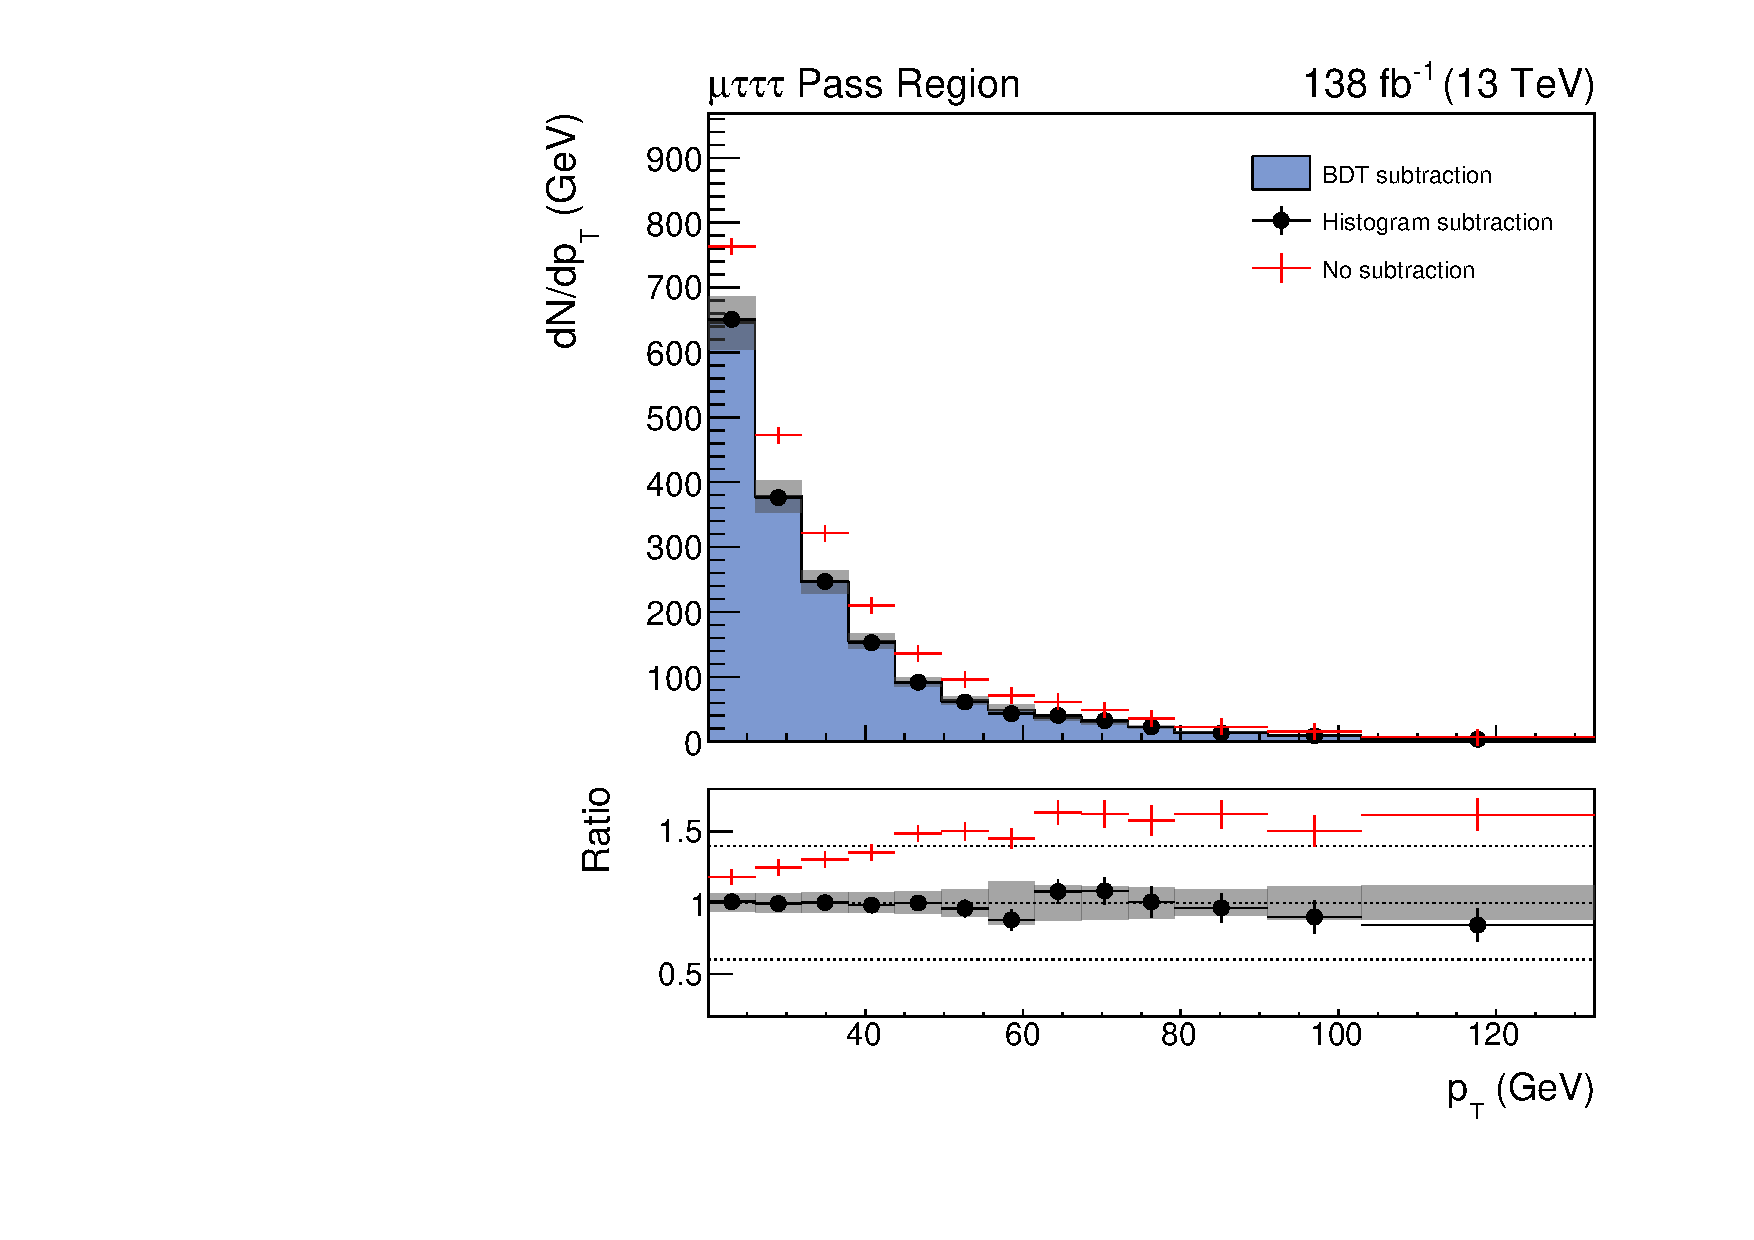
\includegraphics[width=0.45\textwidth]{Figures/subtraction_plot_pt_1_mttt_pass.pdf}}
    \subfloat[]{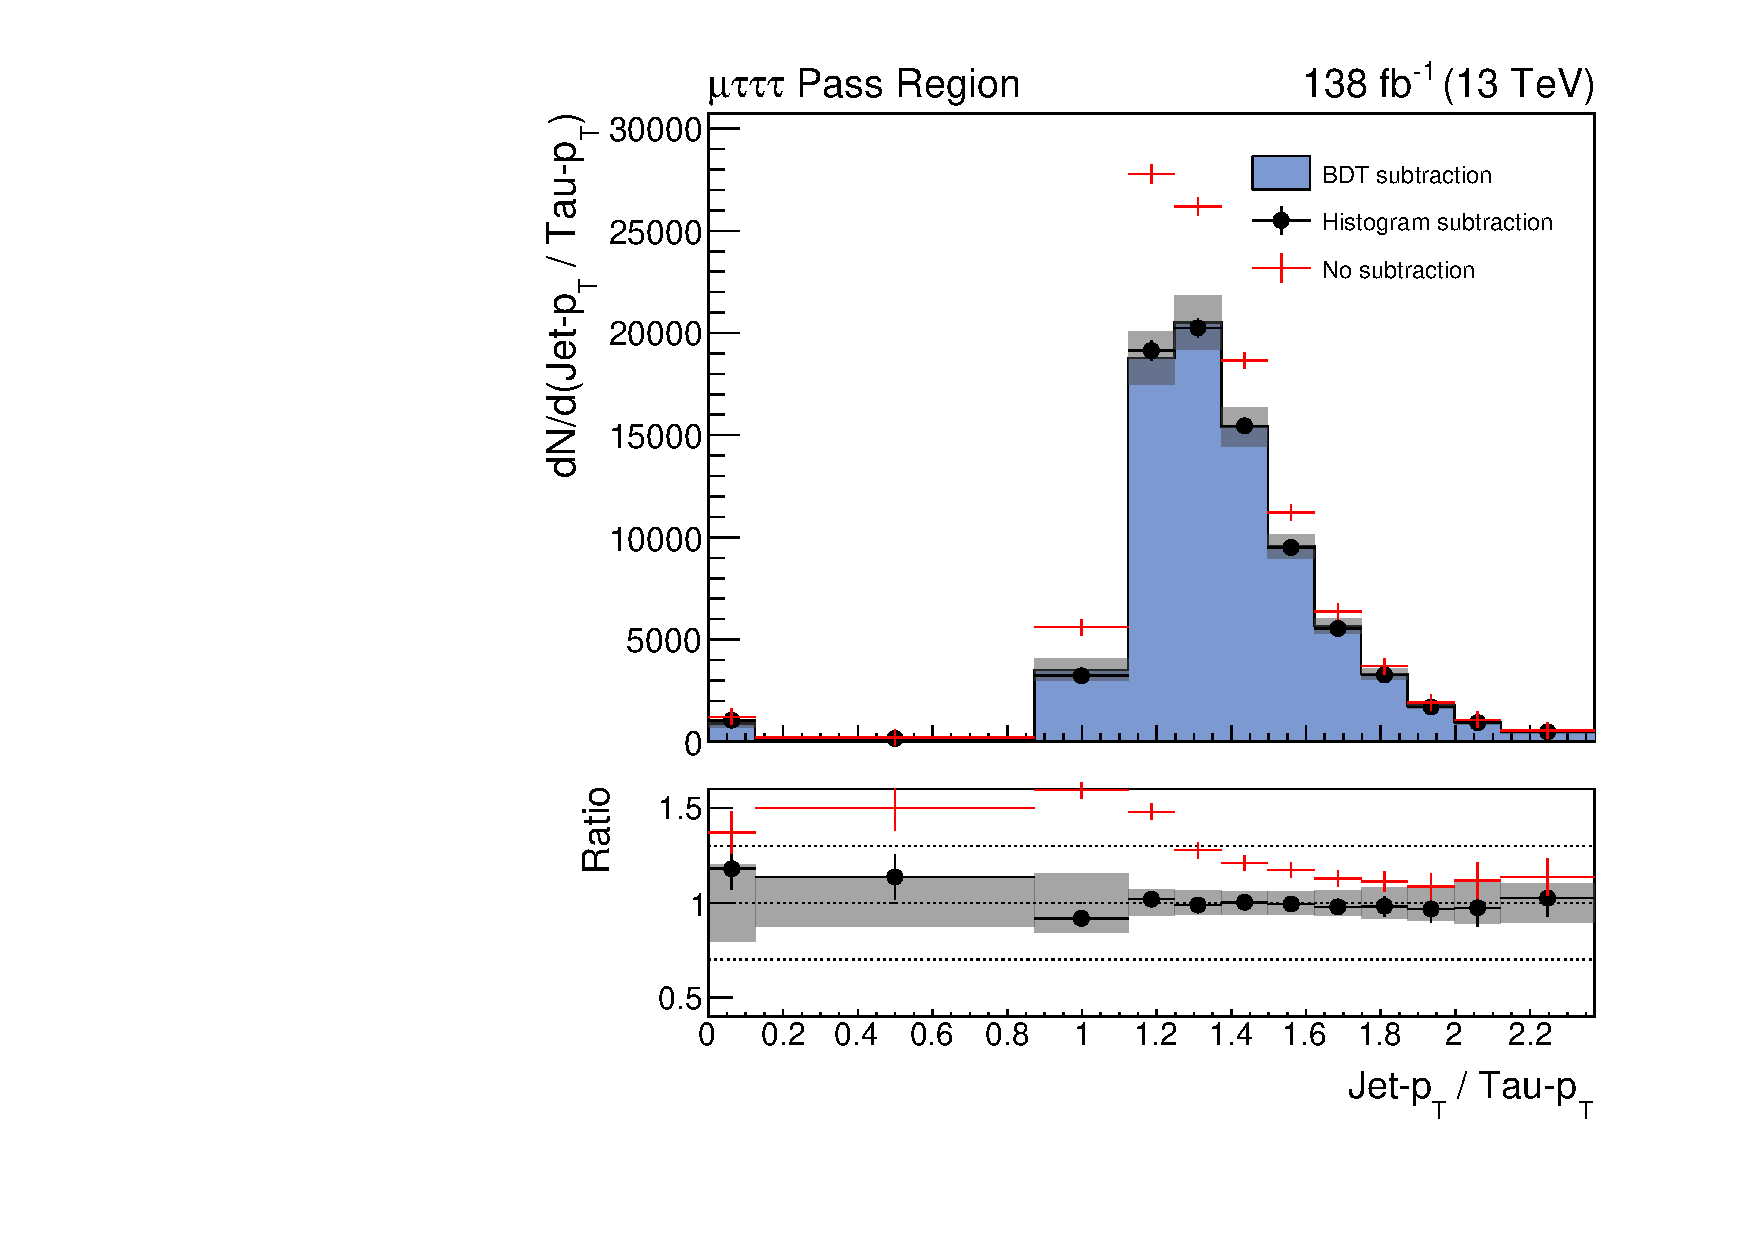
\includegraphics[width=0.45\textwidth]{Figures/subtraction_plot_jet_pt_1_divide_pt_1_mttt_pass.pdf}} \\
    \subfloat[]{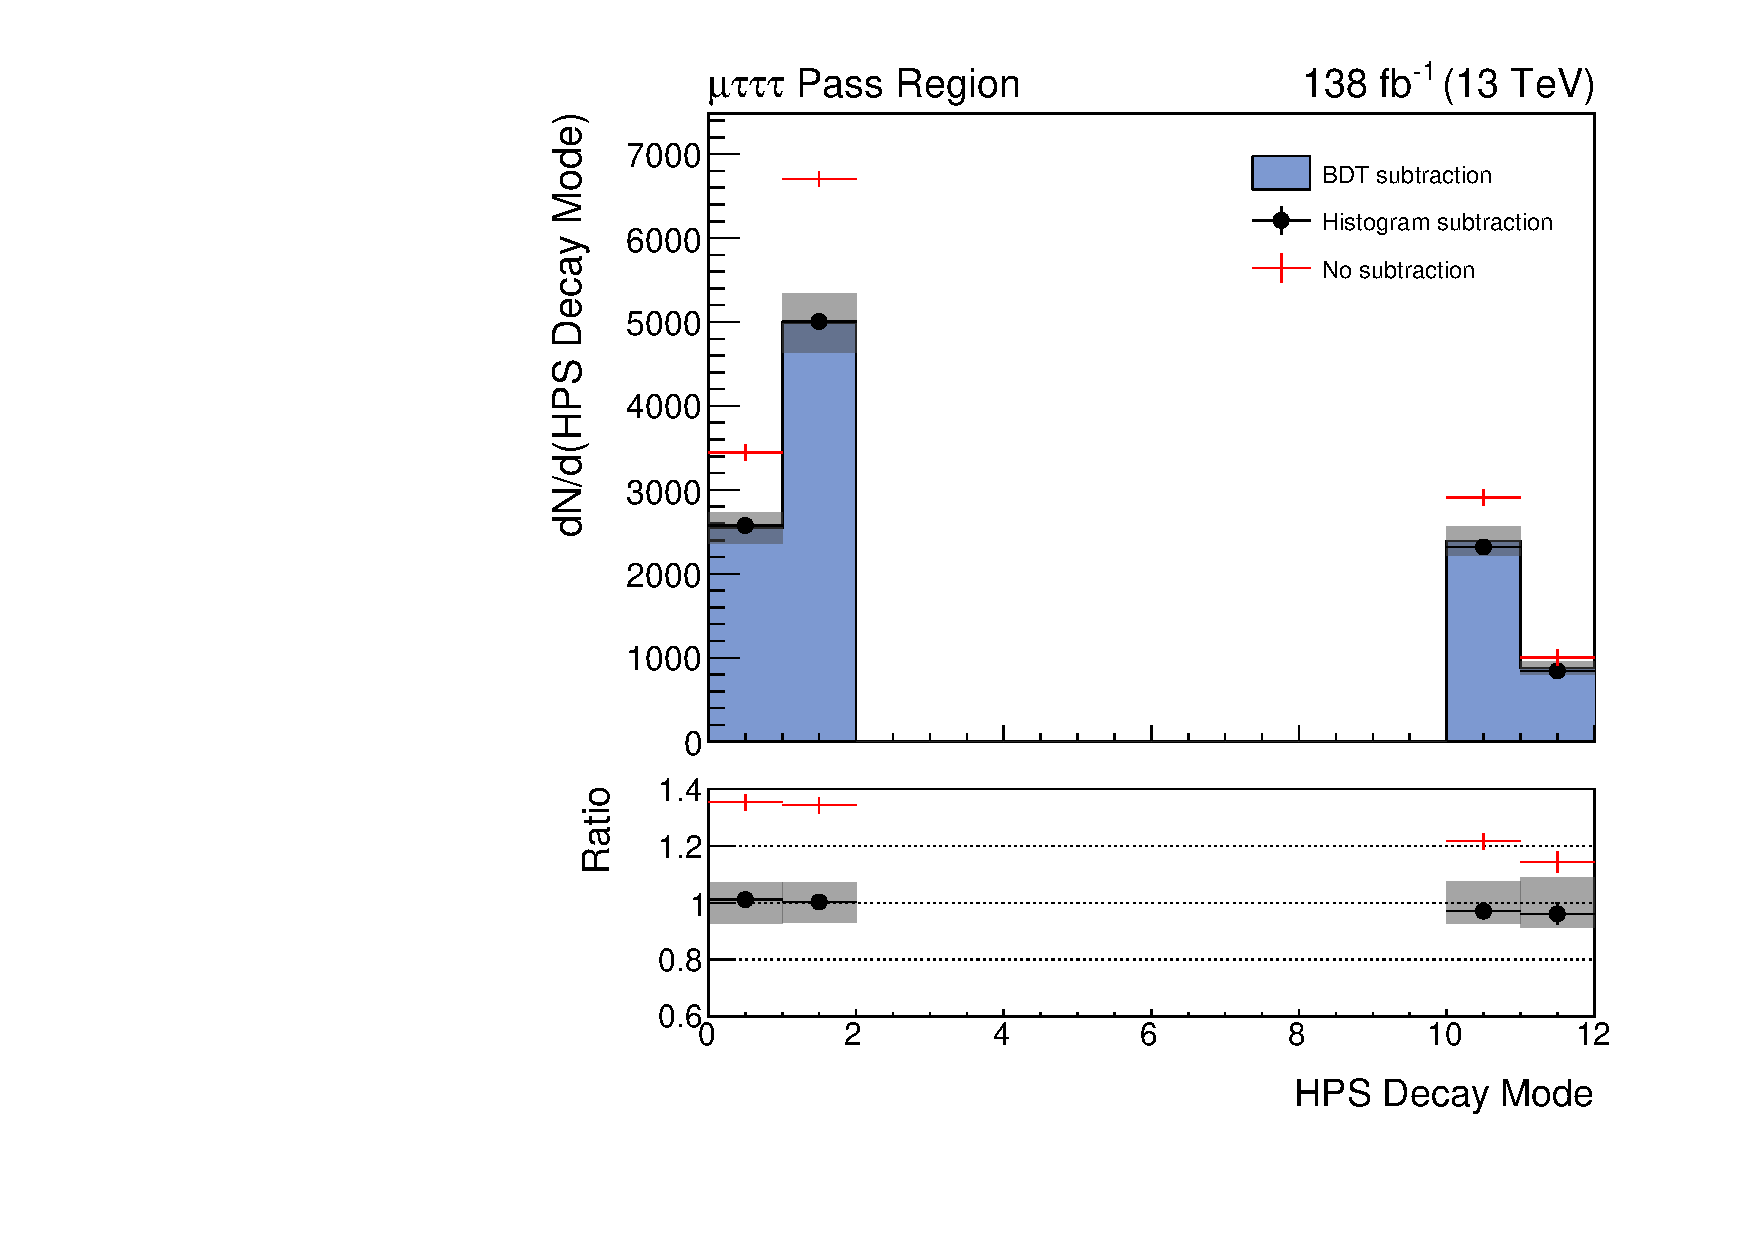
\includegraphics[width=0.45\textwidth]{Figures/subtraction_plot_tau_decay_mode_1_mttt_pass.pdf}}
    \subfloat[]{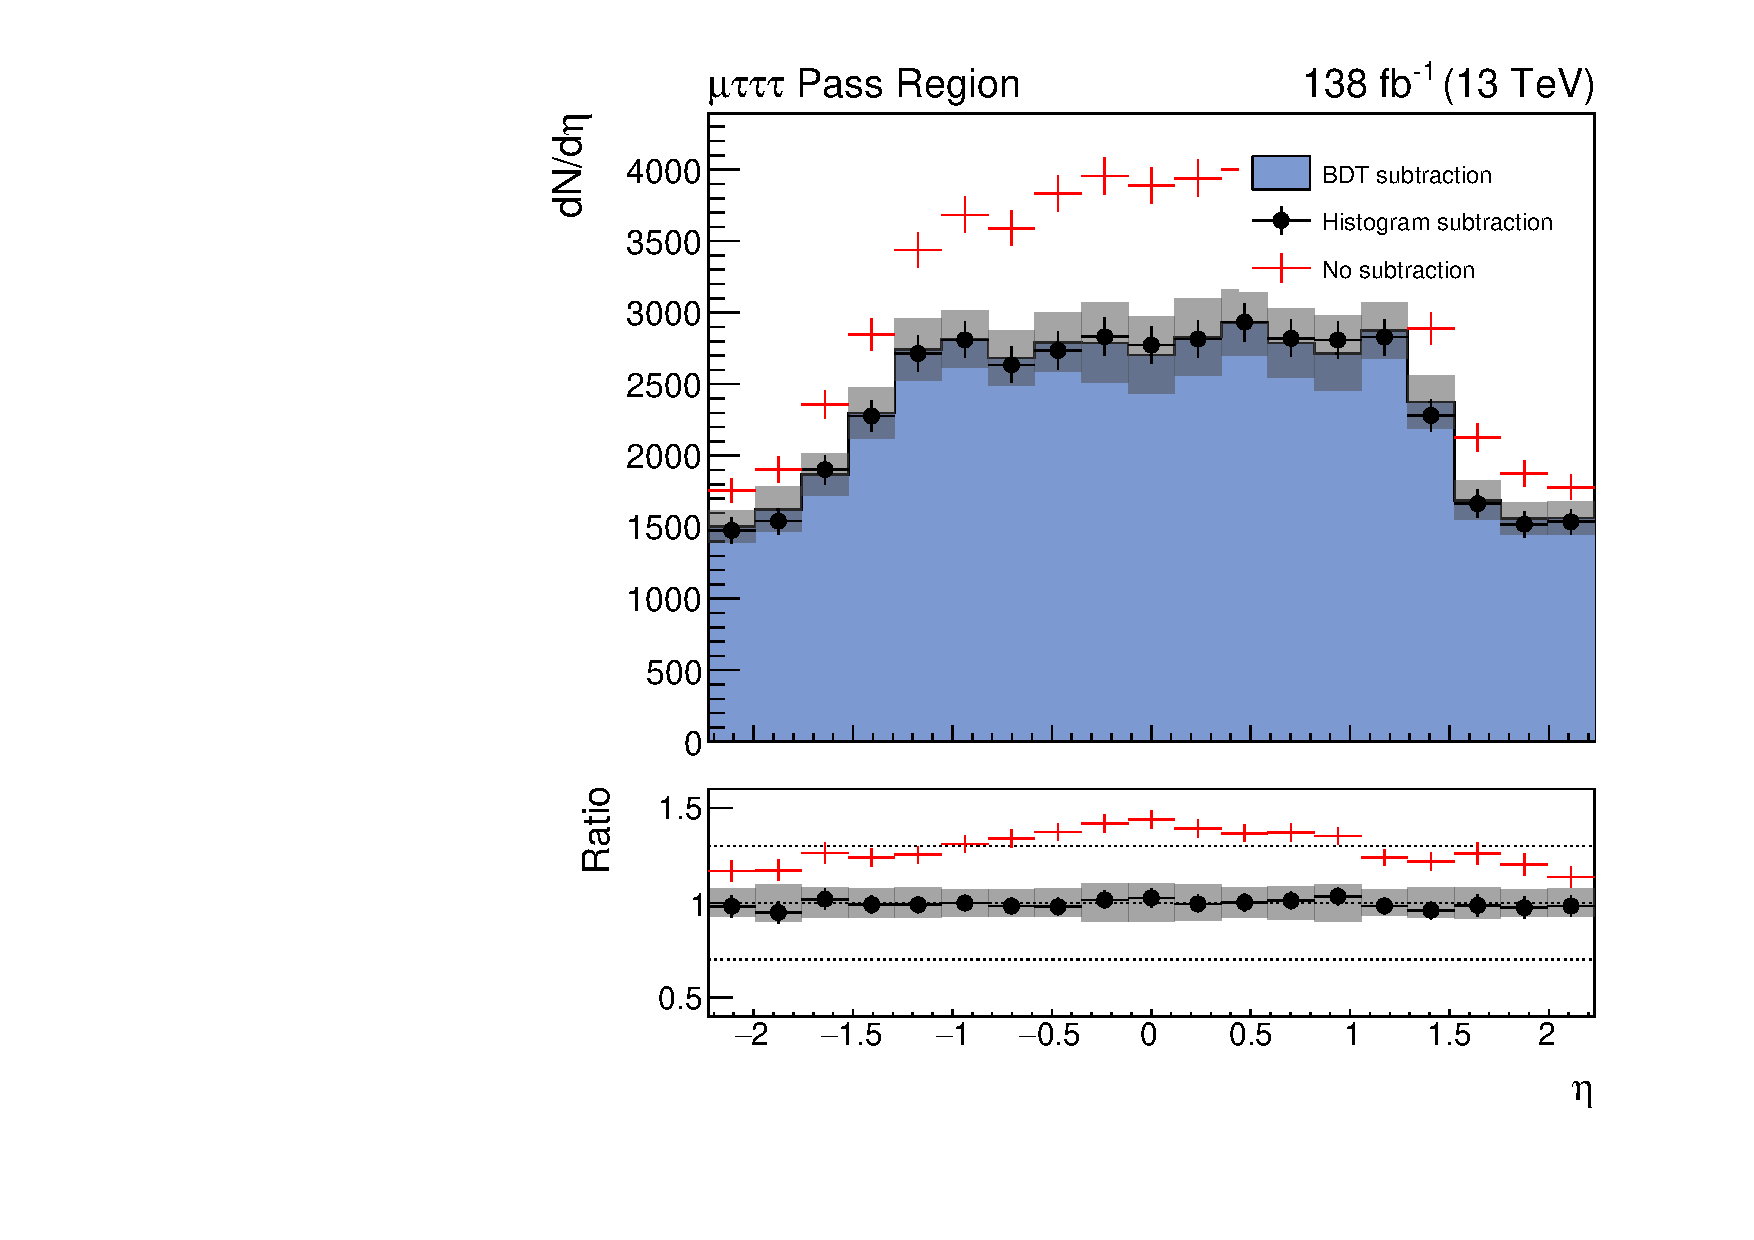
\includegraphics[width=0.45\textwidth]{Figures/subtraction_plot_eta_1_mttt_pass.pdf}}
\caption{Comparison of histograms produced via the BDT subtraction method to histogram subtraction. Also shown is the histogram produced when no subtraction is performed. The uncertainty bands contain statistical uncertainties and uncertainties derived on the non-closure of the method The is shown for four of the fitted variable: $\tauh$-$\pT$, the ratio of $\tauh$-$\pT$ to jet-$\pT$, the $\tauh$ HPS decay mode and the $\tauh$-$\eta$.}
\label{fig:4tau_ff_subtraction}
\end{figure}

\subsection{Fitting}

These subtracted datasets are then randomly split 50:50 into a train and test datasets and only the train dataset is fit. 
The BDT reweighter has a number of hyperparameters and these are tuned with a scan optimising the Kolomogrov-Smirnoff test \cite{} on the test dataset in each channel separately.
Final models are then produced that can optimally model jet $\rightarrow\tauh$ candidates for all fitted variables. 
Examples of the fake factor derived in the $\mu\tauh\tauh\tauh$ channel are shown in Figure~\ref{fig:4tau_ff_reweights}. \\

\begin{figure}[!hbtp]
\centering
    \subfloat[]{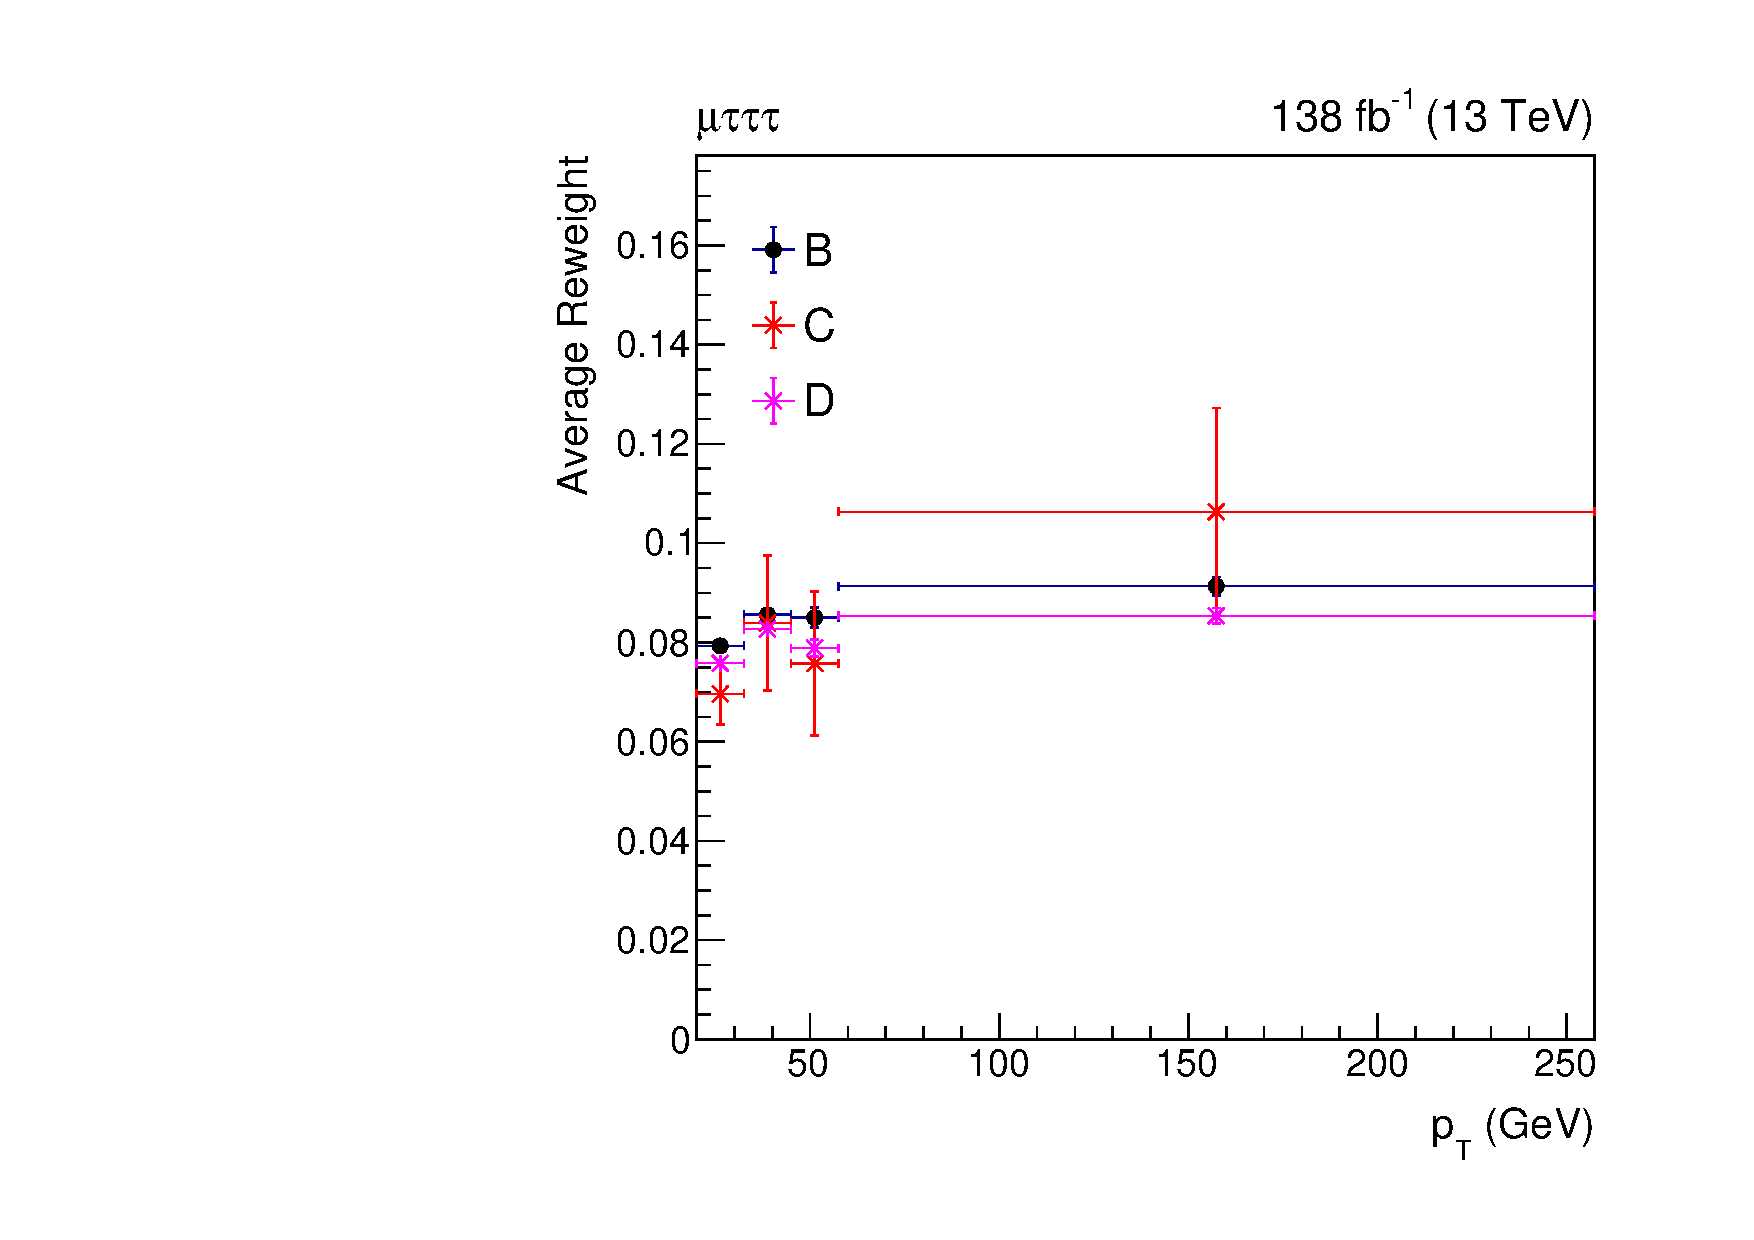
\includegraphics[width=0.45\textwidth]{Figures/reweight_ave_plot_pt_1_all_mttt_all_years.pdf}}
    \subfloat[]{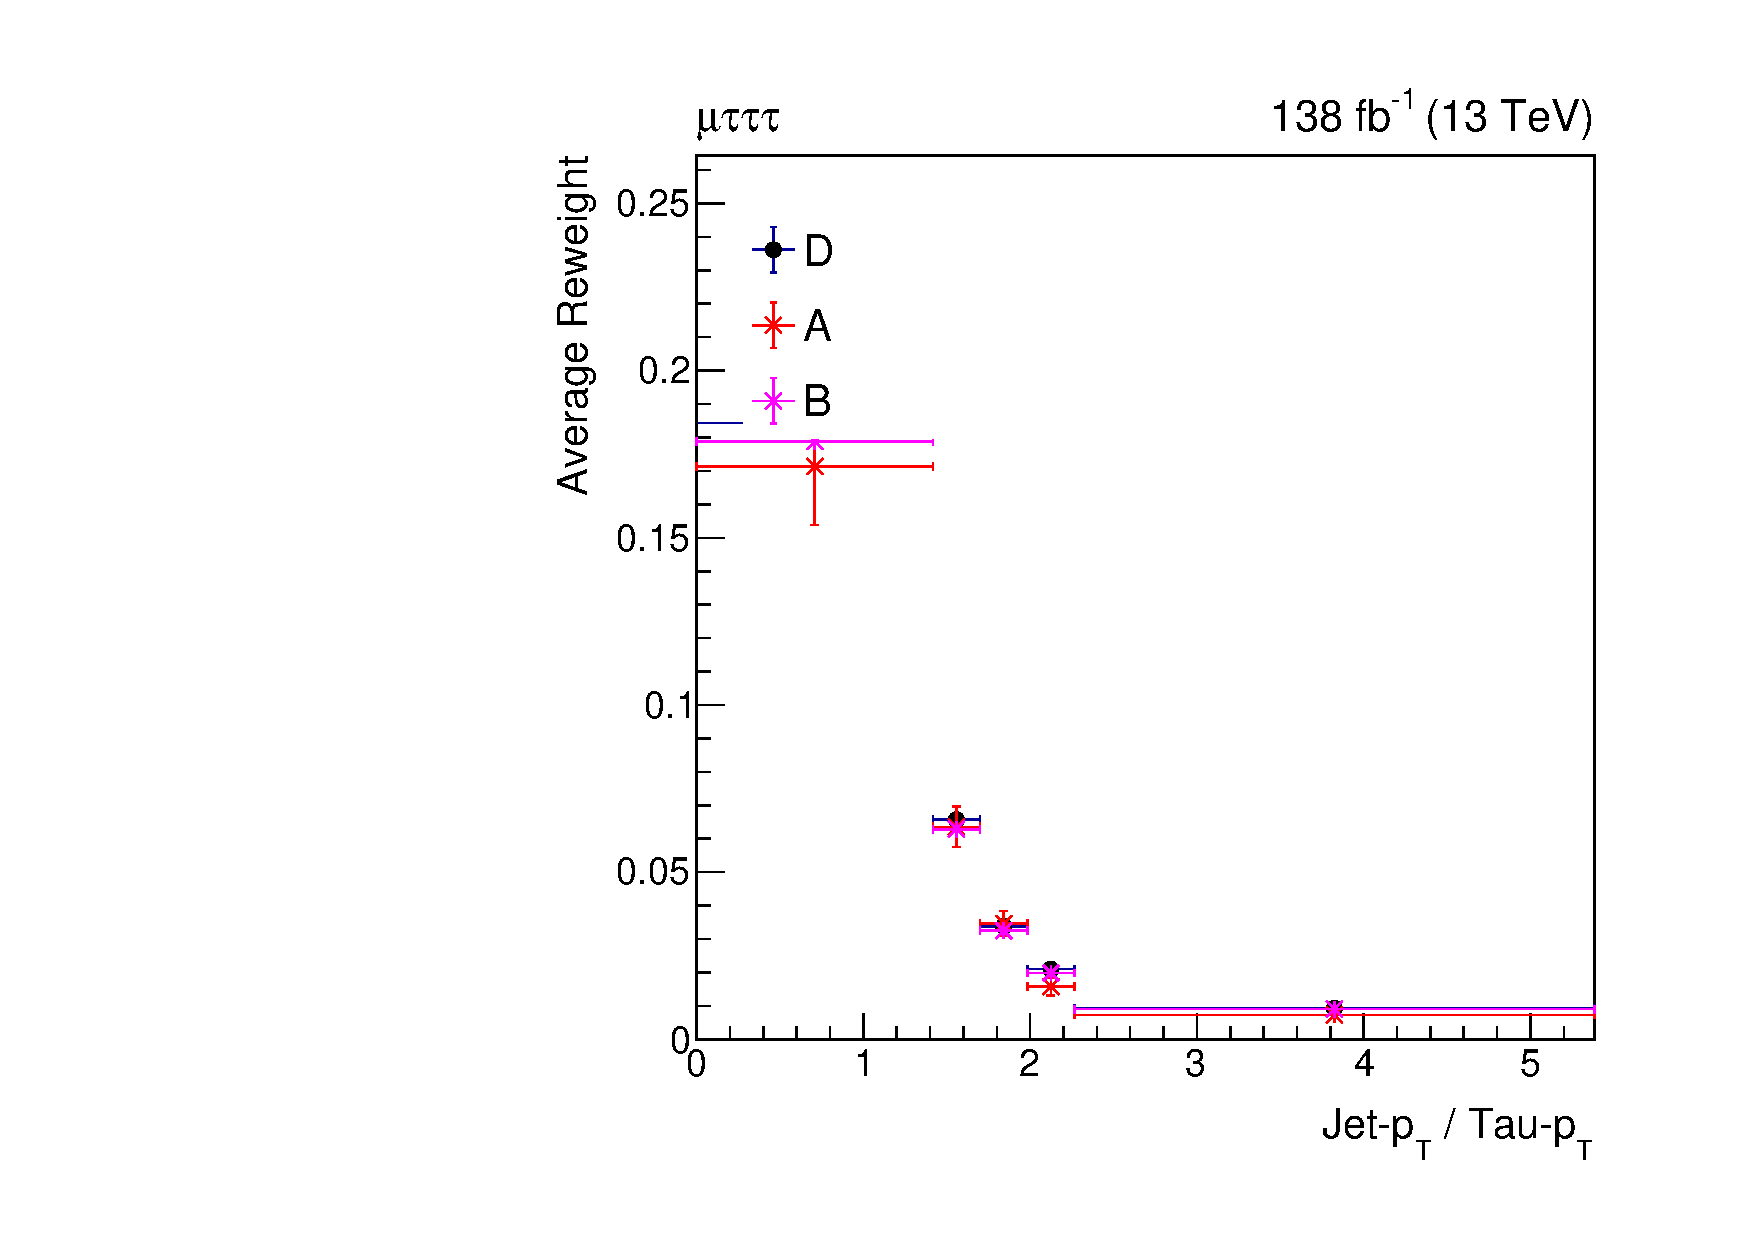
\includegraphics[width=0.45\textwidth]{Figures/reweight_ave_plot_jet_pt_1_divide_pt_1_all_mttt_all_years.pdf}} \\
    \subfloat[]{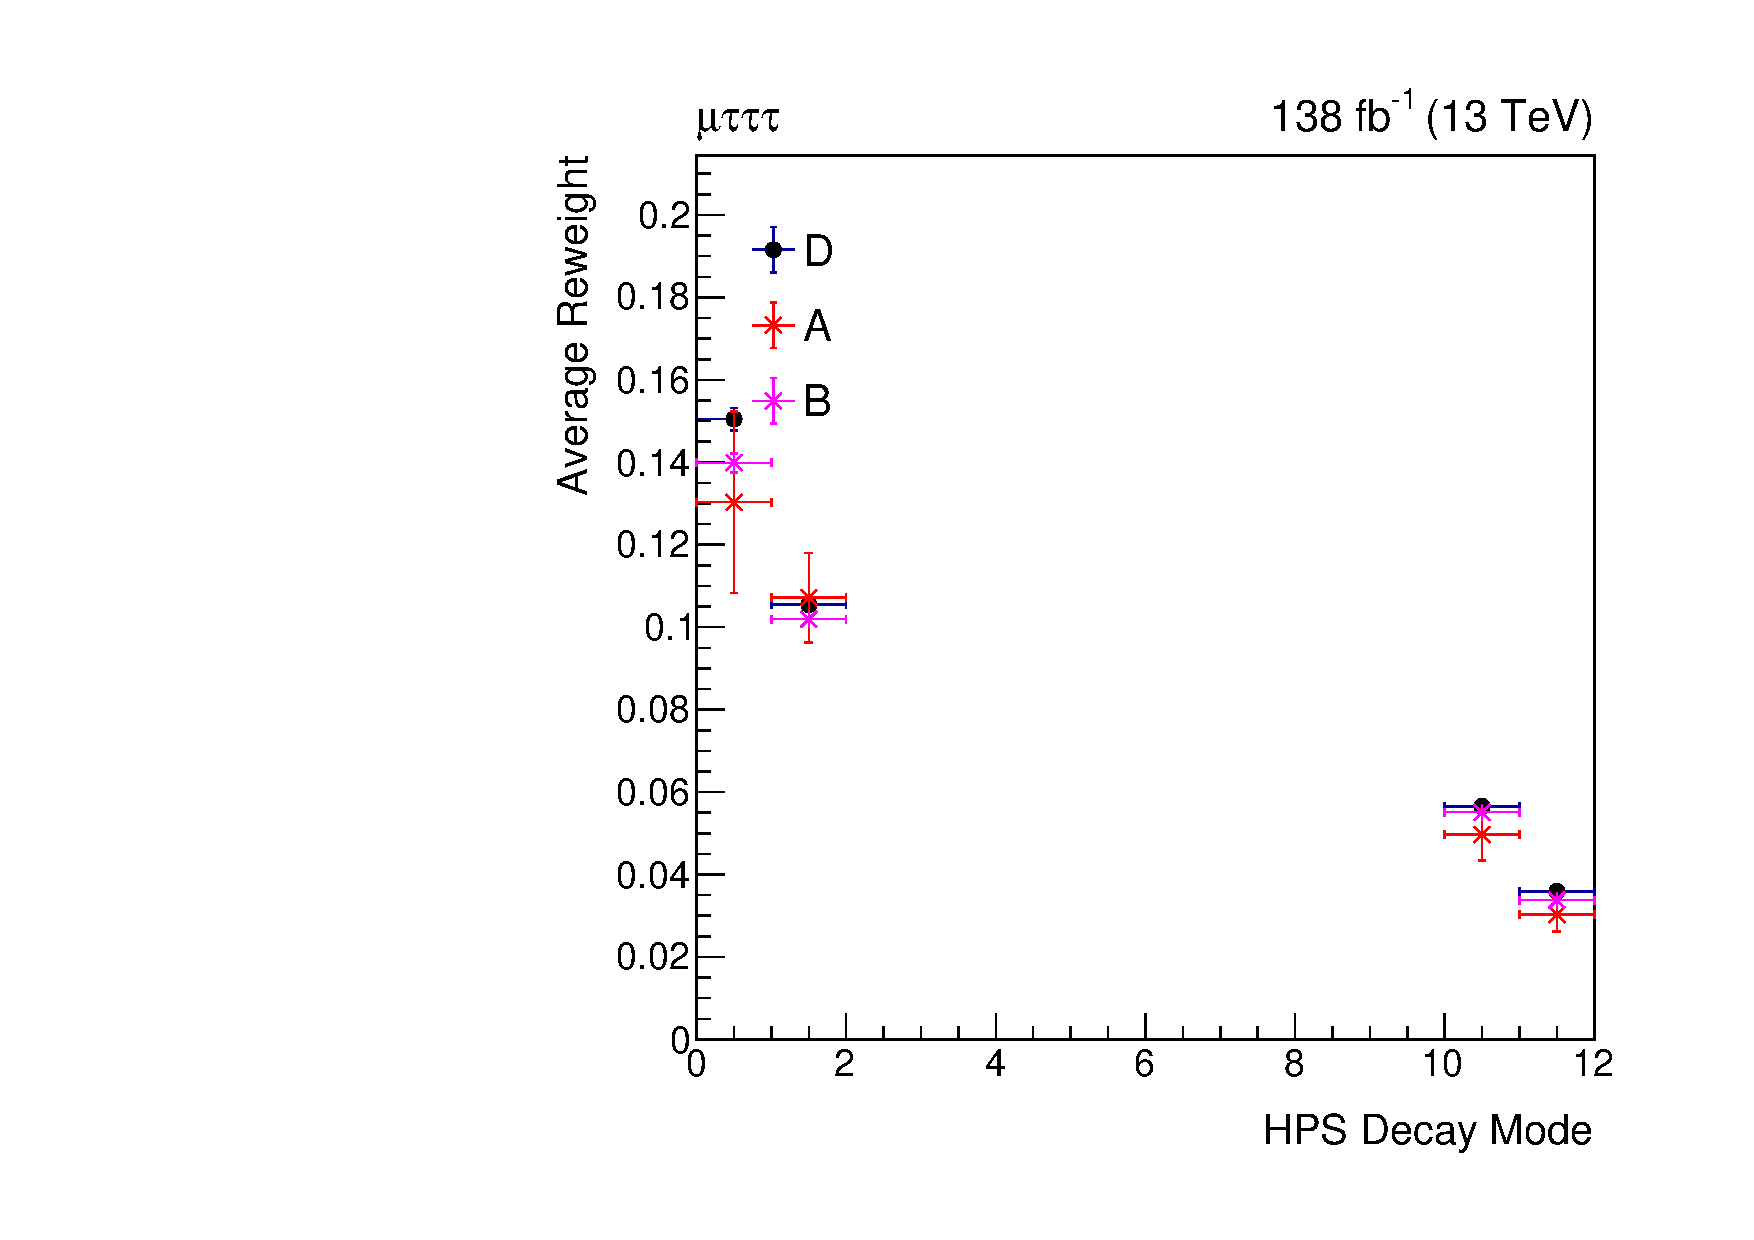
\includegraphics[width=0.45\textwidth]{Figures/reweight_ave_plot_tau_decay_mode_1_all_mttt_all_years.pdf}}
    \subfloat[]{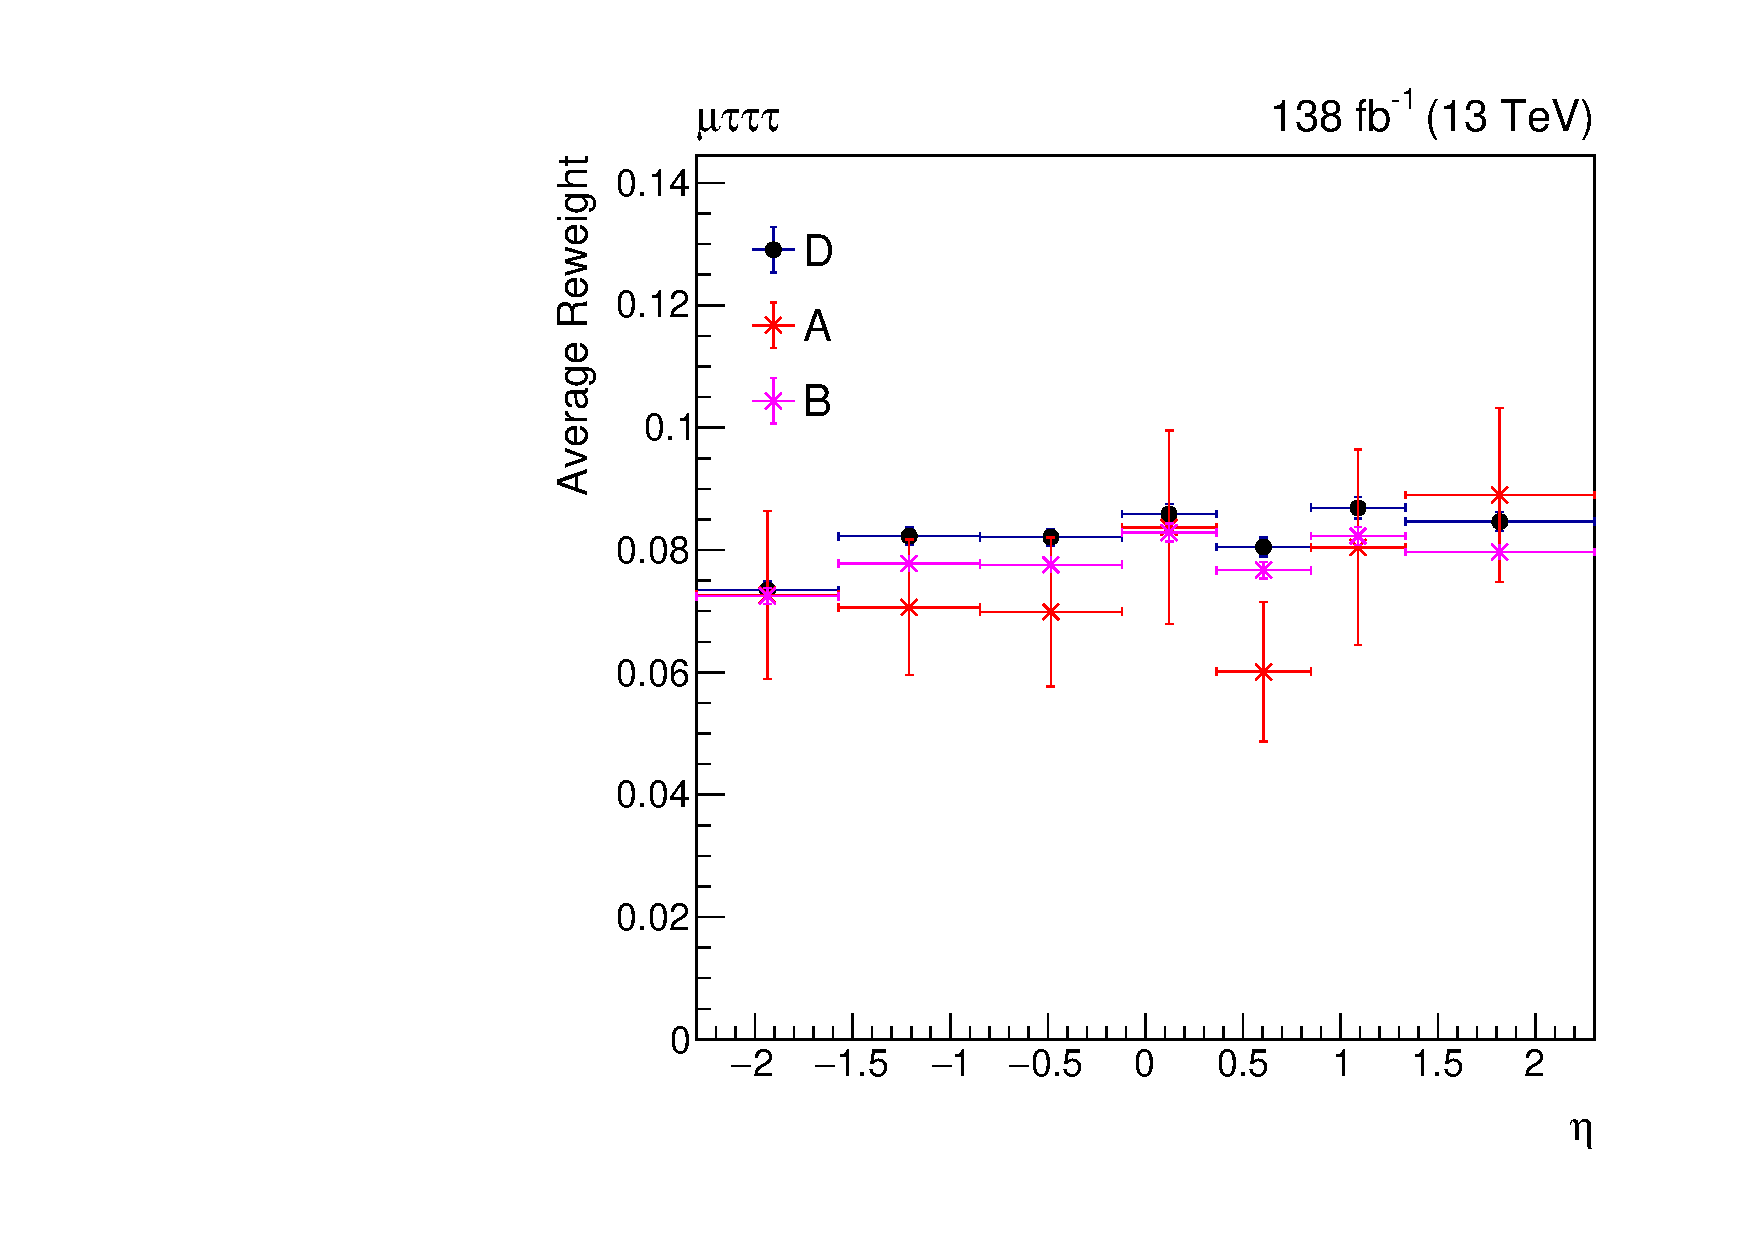
\includegraphics[width=0.45\textwidth]{Figures/reweight_ave_plot_eta_1_all_mttt_all_years.pdf}}
\caption{Average fake factors (reweights) calculated by the BDT reweighting method shown individually in regions A, B and D NEED TO CHANGE THE REGIONS as defined in Figure~\ref{fig:ff_schematic}. The is shown for four of the fitted variable: $\tauh$-$\pT$, the ratio of $\tauh$-$\pT$ to jet-$\pT$, the $\tauh$ HPS decay mode and the $\tauh$-$\eta$.}
\label{fig:4tau_ff_reweights}
\end{figure}

An uncertainty is placed on the performance of this algorithm.
This is again calculated by drawing each variable into a histogram and comparing the histograms from reweighted events with the alternative $\tauh$ ID selections to the events with the nominal $\tauh$ ID in all of the fitted regions simultaneously.
Plots of the closure of this method in the $\mu\tauh\tauh\tauh$ accompanied by this uncertainty are shown in Figure~\ref{fig:4tau_ff_closure}. \\

\begin{figure}[!hbtp]
\centering
    \subfloat[]{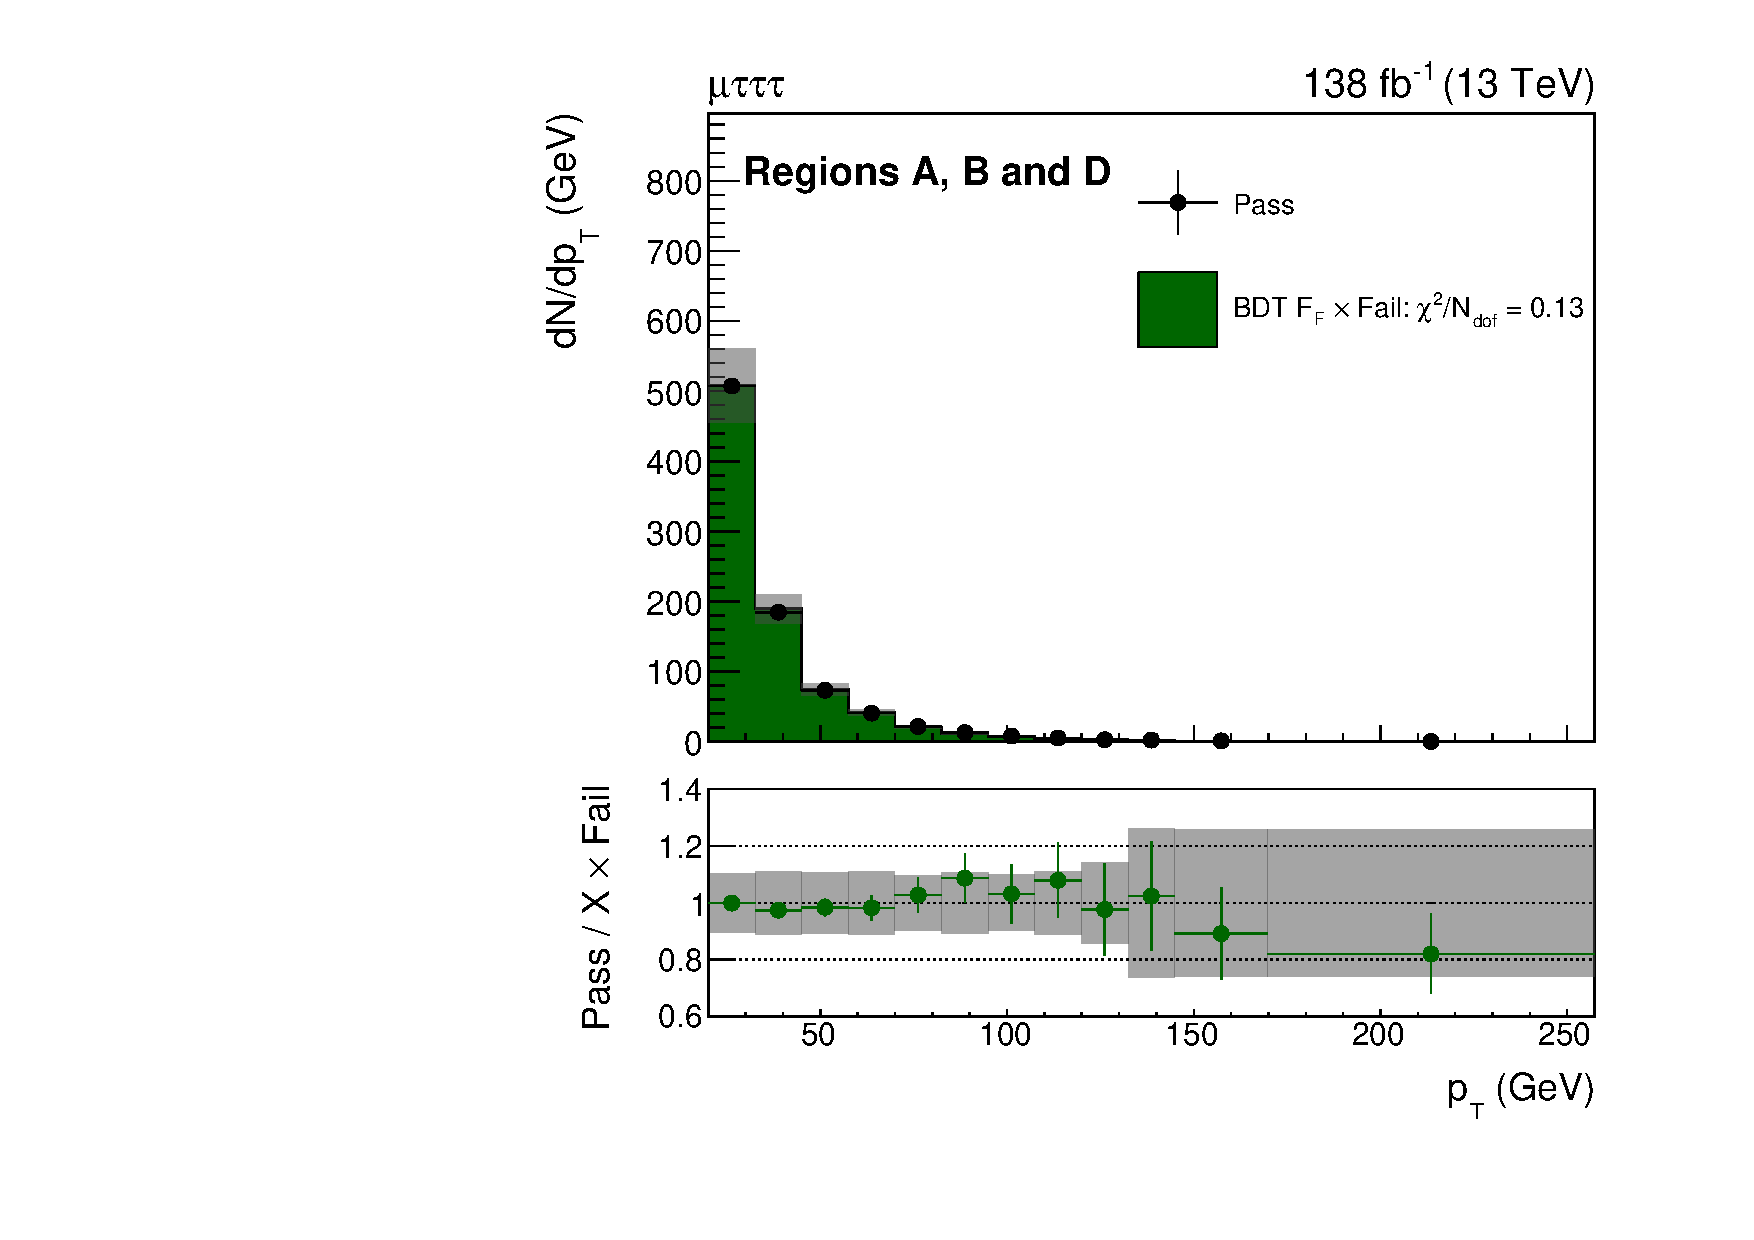
\includegraphics[width=0.45\textwidth]{Figures/closure_plot_pt_1_all_mttt_all_years_all.pdf}}
    \subfloat[]{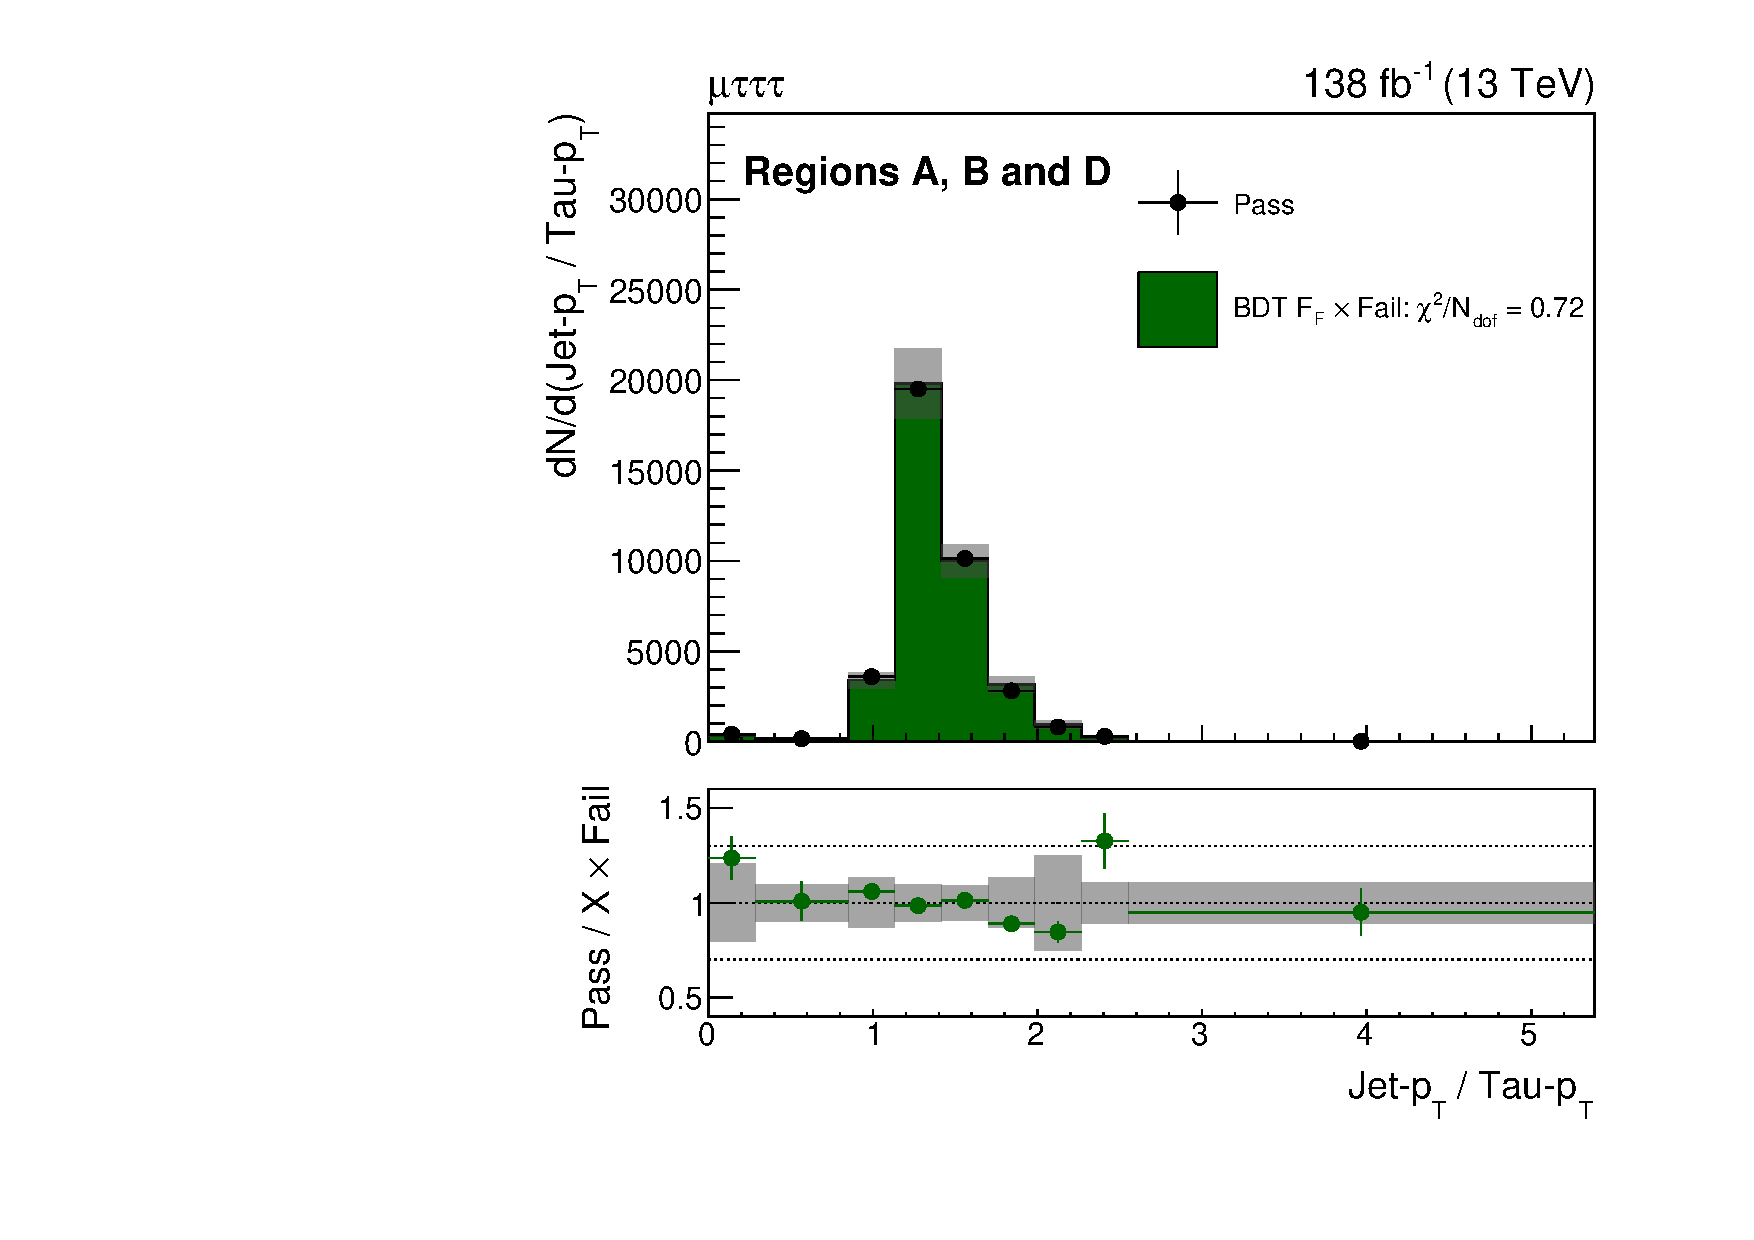
\includegraphics[width=0.45\textwidth]{Figures/closure_plot_jet_pt_1_divide_pt_1_all_mttt_all_years_all.pdf}} \\
    \subfloat[]{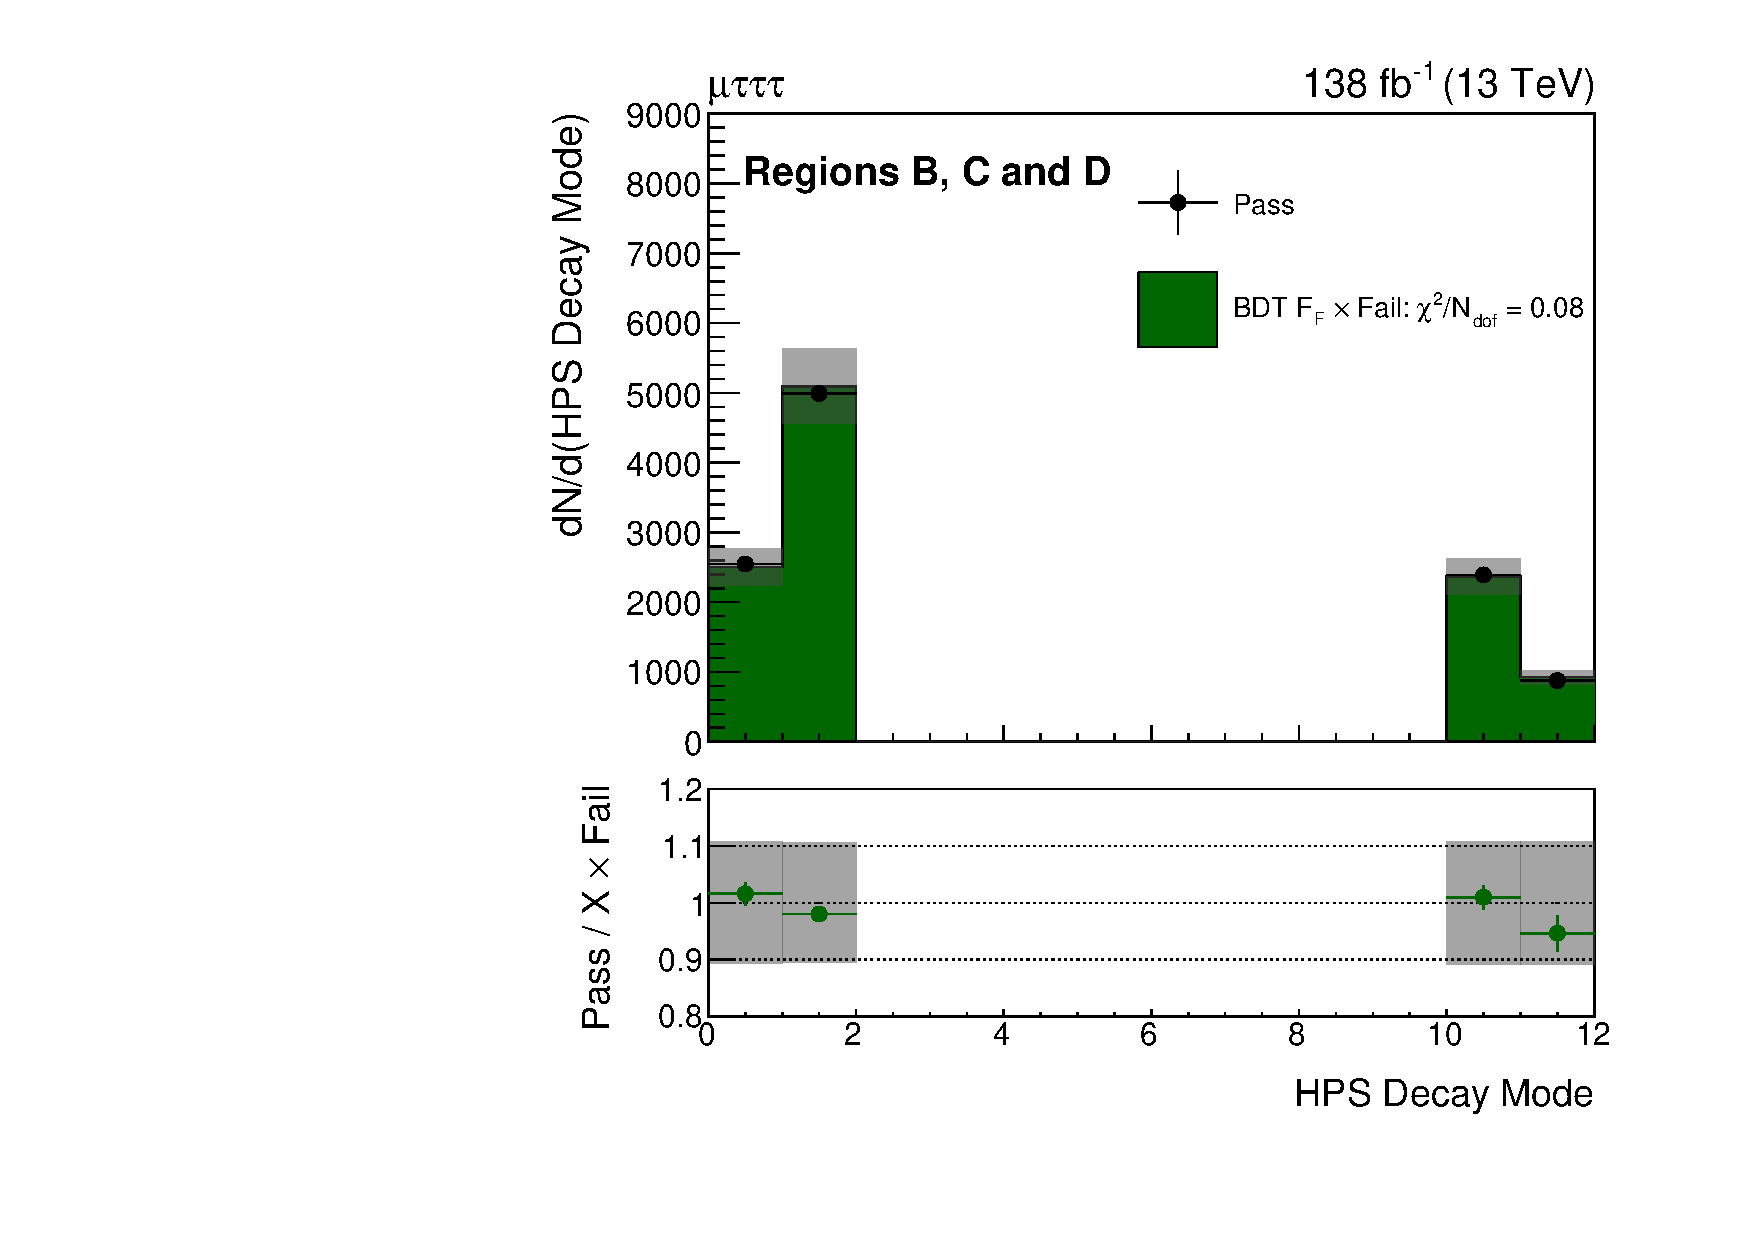
\includegraphics[width=0.45\textwidth]{Figures/closure_plot_tau_decay_mode_1_all_mttt_all_years_all.pdf}}
    \subfloat[]{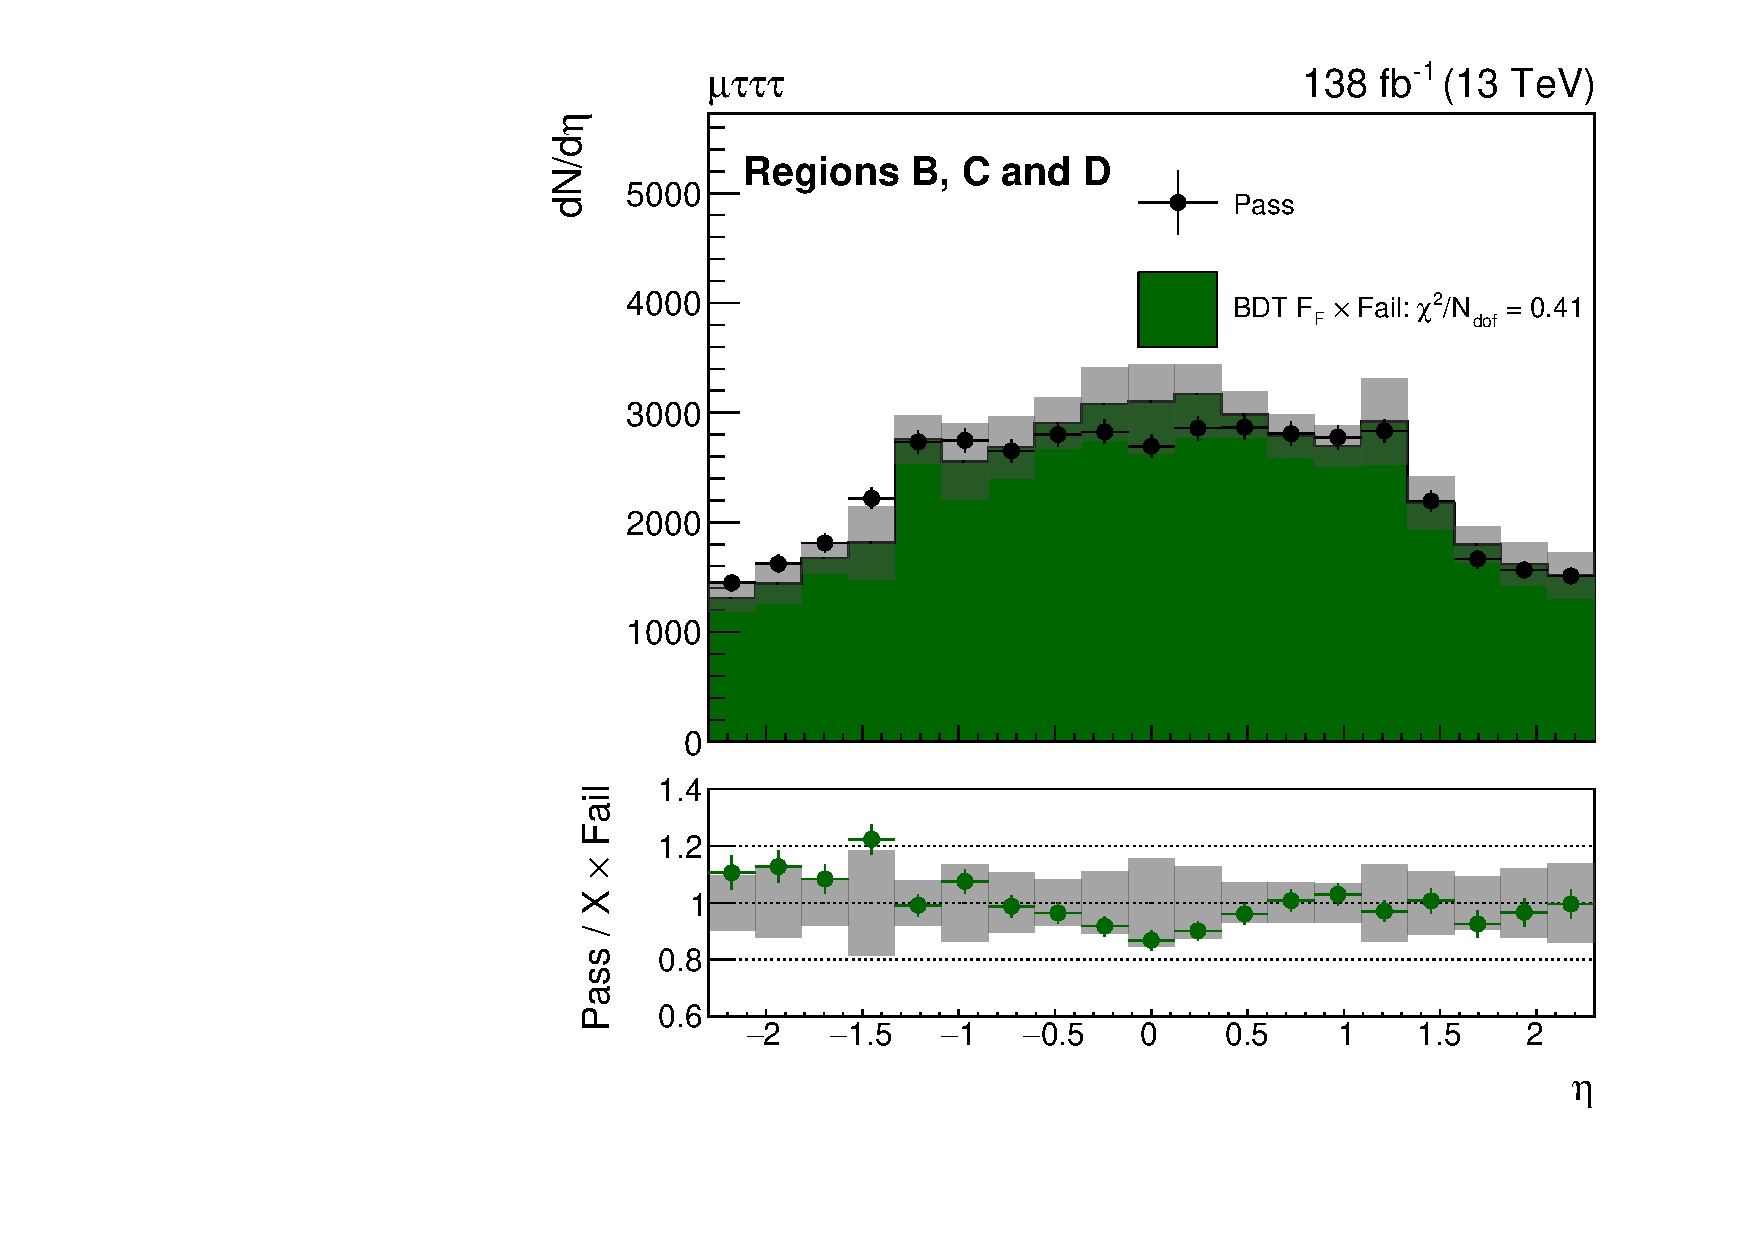
\includegraphics[width=0.45\textwidth]{Figures/closure_plot_eta_1_all_mttt_all_years_all.pdf}}
\caption{Comparison of histograms produced using the fake factors applied to the fitted fail region compared to fitted pass region. The uncertainty bands contain statistical uncertainties and uncertainties derived on the non-closure of the method. The is shown for three of the fitted variable: $\tauh$-$\pT$, the ratio of $\tauh$-$\pT$ to jet-$\pT$, the $\tauh$ HPS decay mode and the $\tauh$-$\eta$. The $\chi^2$ divided by number of degrees of freedom between the two histograms is also shown.}
\label{fig:4tau_ff_closure}
\end{figure}

\subsection{Applying Fake Factors}

Fake factors, $F_{F}^{i}$, have now been calculated for each $\tauh$ candidate, $i$, in the event and uncertainties determined on each weight. 
However, it is difficult to generate a full description of any number of jet $\rightarrow \tauh$ fakes in an event.
Taking channels with two $\tauh$ candidates as the simplest example, if the jet $\rightarrow \tauh$ background is determined purely off the leading $\tauh$ candidate, then events the leading $\tauh$ is genuine and the sub-leading $\tauh$ is a jet, are missed.
Similarly, the situation can be flipped if the sub-leading $\tauh$ is chosen to determine the jet $\rightarrow \tauh$ fake background.
A third options can be tried where both $\tauh$ candidates are used to determine the background.
However, this will only model events where both $\tauh$ candidates are jets and not where there is a single jet $\rightarrow \tauh$ fake. 
It is seen that if the first two attempts at calculating this background from individual candidates are added and the contribution from both $\tauh$ candidates is subtracted, all possible numbers of jet fakes in the event are accounted for. \\

\begin{table}[H]
\centering
\begin{tabular}{|l|ccc|}
\hline
Region    & $\tauh^1 (\tau) \tauh^2 (j)$ & $\tauh^1 (j) \tauh^2 (\tau)$ & $\tauh^1 (j) \tauh^2 (j)$ \\
\hline
\hline
$R_{1}$ (from $\tauh^1$)     & 0                            & 1                            & 1                         \\
$R_{2}$ (from $\tauh^2$)     & 1                            & 0                            & 1                         \\
$R_{12}$ (from both)         & 0                            & 0                            & 1                         \\
\hline
$R_{1} +R_{2} - R_{12}$      & 1                            & 1                            & 1       \\                  
\hline
\end{tabular}
\caption{Regions modelled by the fake factor method when using the leading $\tauh$ ($\tauh^1$), the sub-leading $\tauh$ ($\tauh^2$) and both, to model the jet $\rightarrow \tauh$ background and whether that specific object is a genuine $\tau$ lepton ($\tau$) or a jet ($j$). Also shown is a combination of three regions to fully model all possible combinations. }
\label{tab:apply_ff}
\end{table}

This logic is extended to all channels with one exception.
The $\tau_h \tau_h \tau_h \tau_h$ channel application region would have overlap with the $\tau_h \tau_h \tau_h$ signal region using this common method, therefore the formula is adjusted to avoid this region.
If the overlapped regions are removed from the equation, the scale of the triple and quadruple regions needed to be adjusted to account for this.
The caveat to this is that events where there are only one jet $\rightarrow \tauh$ candidate are not accounted for.
As the majority of the background events in this channel comes from QCD with many jet $\rightarrow \tauh$ candidates, this contribution is deemed negligible.
The formulae for the total jet $\rightarrow \tauh$ backgrounds in each channel are shown below. \\

\begin{enumerate}[i)]
\item $\mu\mu\tauh\tauh$, $ee\tauh\tauh$ and $e\mu\tauh\tauh$
\begin{equation}
R_1 + R_2 - R_{12}
\end{equation}

\item $\mu\tauh\tauh\tauh$, $e\tauh\tauh\tauh$ and $\tauh\tauh\tauh$
\begin{equation}
R_1 + R_2 + R_3 - R_{12} - R_{13} - R_{23} + R_{234}
\end{equation}

\item $\tauh\tauh\tauh\tauh$
\begin{align}
\begin{split}
&R_{12} + R_{13} + R_{14} + R_{23} + R_{24} + R_{34} \\
&- 2(R_{123} + R_{124} + R_{134} + R_{234}) + 3R_{1234}
\end{split}
\end{align}
\end{enumerate}
 
\section{Uncertainty Model}

The uncertainty model follows the schemes detailed in Section~\ref{sec:uncerts} for the statistical uncertainties and systematic uncertainties for light leptons, jets, leptons misidentified as hadronic taus, MET, luminosity and prefiring.
Updates and additions to the previous uncertainty model are shown below. \\

\subsubsection{Hadronic Taus}
An improvement is made to the $\tauh$ ID uncertainty correlation scheme applied to simulated events.
The fit used to derive scale factors for the $\tauh$ MC events consists of both statistical and systematic uncertainties.
In the previous search, the ID uncertainties where correlated across decay mode and era despite the statistical components of each fit begin orthogonal.
Therefore for this search the uncertainty scheme contains correlated and decorrelated part across decay and era.
The double-$\tauh$ trigger uncertainties remain unchanged. \\

\subsubsection{Jets misidentified as hadronic taus}
The backgrounds with jets misidentified as $\tauh$ are estimated from data with the ML fake factor method. 
There are different sources of uncertainty related to this method. 
All uncertainties are uncorrelated across decay channels, except in the $\tauh\tauh\tauh\tauh$ and $\tauh\tauh\tauh$ where the same fit is used, so uncertainties are correlated. \\

The initial uncertainties come from removal of the non jet$\rightarrow\tauh$ backgrounds from the fitting region and this is split into two types.
Firstly, an uncertainty is placed on the non-closure of the BDT subtraction method, this is done by comparing the distributions in each variable fit using standard histogram subtraction with the BDT subtraction method, and the largest shift is taken for each event. This is done separately in the pass and fail $\tauh$ ID regions.
The second uncertainty to do with purify the fitting region is motivated by any MC mismodelling of the non jet$\rightarrow\tauh$ objects predicted.
This is shifted up and down by 10\%, to represent any MC mismodelling , and the BDT subtraction method and the reweighting is repeated with the differing datasets. \\

The second source of uncertainties comes from the BDT reweighter fit.
In a similar way to the subtraction method, an uncertainty is placed on the non closure of the fit, comparing reweighted events in the fail $\tauh$ ID region to the pass $\tauh$ ID region.
Further uncertainties are placed on the assumption of the variables used to separate the signal region from the fitting region.
The assumption is that the fake factors would be identical no matter what combination of these variables are used.
Therefore, the uncertainties are placed by taking the largest shift when changing these variables whilst getting the output to the fit.
These are decorrelated in each combination of the separating variables.

\subsubsection{Background process specific uncertainties}
Specific uncertainties are placed on the di-Z simulated events due to application of k factors.
Due to the size of the differences between NNLO and lower order predictions for the cross sections, an uncertainty is placed on the size of these yields utilising the k factors derived.

\subsubsection{Signal process specific uncertainties}
PDF, $\alpha_s$ and $\mu_{R}$/$\mu_{F}$ scale variations are applied on an event-by-event basis to the signal samples.
The normalisation of these uncertainties are approximately 6\%, 1\% and 2\% respectively.

\section{Signal Extraction}

The statistical interpretation of the results is done as described in Section~\ref{sec:sig_ext}, but with different signal scaling functions, $g$, and parameters of interest, $\mu$.
The two interpretation of the analysis, as stated at the beginning of chapter, have different parameters of interest and scaling functions. \\

Firstly, the model independent search uses a linear scaling function, $g(\mu)=(\mu)$, and a parameter of interest that represents the cross section of the $Z^{*}\rightarrow \phi A$ multiplied by the branching fractions of $\phi\rightarrow\tau\tau$ and $A\rightarrow\tau\tau$.
Secondly, the interpretation in the type X 2HDM model is done by testing each point in the parameter space, whether that ia $m_{A}$-$\tan\beta$ for the alignment scenario or $\cos(\beta-\alpha)$-$\tan\beta$ for scenarios of the remaining parameters. 
This is done by scaling the samples to the predicted cross sections times branching ratios at that point in the parameter space, and defining a single rate parameter that can only take the values 1 (type X 2HDM) and 0 (SM) with $g(\mu)=\mu$.

\subsection{Postfit Plots}

Tab.~\ref{tab:sig_integrals} shows the unblinded event yields in each analysis category, alongside the number of bins fit, the background prediction and uncertainties split in statistical and systematic contributions after a background-only fit and a signal yield prediction.
Fig.~\ref{fig:4tau_postfit} show the unblinded distributions in channels where more than one bin is fit.
SIGNAL HYPOTHESIS PLOT \\

DISCUSS RESULTS \\

\begin{table}[h]
\centering
\resizebox{\textwidth}{!}{
\begin{tabular}{|l||c|c|c|c|}
\hline
  Category & $N_{\text{bins}}$ & Total Background & Data Observed & $(m_{A},m_{\phi}) = (160,300)$ GeV \\ \hline \hline
 & & & & \\
 $\tau_{h}\tau_{h}\tau_{h}\tau_{h}$ & 1 & $10.9$ $\pm$ $3.5$ (stat) $^{+1.9}_{-2.0}$ (syst) & $-$ & $26.1$\\
 & & & & \\
 $\tau_{h}\tau_{h}\tau_{h}$ & 17 & $4790.0$ $\pm$ $85.7$ (stat) $^{+1417.2}_{-1416.0}$ (syst) & $-$ & $94.5$\\
 & & & & \\
 $e\tau_{h}\tau_{h}\tau_{h}$ & 1 & $21.6$ $\pm$ $4.2$ (stat) $^{+8.6}_{-8.6}$ (syst) & $-$ & $26.8$\\
 & & & & \\
 $\mu\tau_{h}\tau_{h}\tau_{h}$ & 1 & $22.0$ $\pm$ $3.5$ (stat) $^{+3.3}_{-3.4}$ (syst) & $-$ & $30.7$\\
 & & & & \\
 $ee\tau_{h}\tau_{h}$ Opposite Sign Leptons & 11 & $243.1$ $\pm$ $11.1$ (stat) $^{+41.7}_{-49.7}$ (syst) & $265$ & $7.0$\\
 & & & & \\
 $ee\tau_{h}\tau_{h}$ Same Sign Leptons & 1 & $3.6$ $\pm$ $1.1$ (stat) $^{+0.5}_{-0.5}$ (syst) & $-$ & $3.7$\\
 & & & & \\
 $\mu\mu\tau_{h}\tau_{h}$ Opposite Sign Leptons & 14 & $369.0$ $\pm$ $13.6$ (stat) $^{+52.6}_{-93.5}$ (syst) & $413$ & $9.4$\\
 & & & & \\
 $\mu\mu\tau_{h}\tau_{h}$ Same Sign Leptons & 1 & $4.8$ $\pm$ $1.7$ (stat) $^{+0.8}_{-1.0}$ (syst) & $-$ & $4.6$\\
 & & & & \\
 $e\mu\tau_{h}\tau_{h}$ Opposite Sign Leptons & 5 & $29.4$ $\pm$ $2.6$ (stat) $^{+1.3}_{-3.6}$ (syst) & $-$ & $16.9$\\
 & & & & \\
 $e\mu\tau_{h}\tau_{h}$ Same Sign Leptons & 3 & $9.7$ $\pm$ $1.4$ (stat) $^{+3.1}_{-3.3}$ (syst) & $-$ & $8.5$\\
 & & & & \\
\hline
\end{tabular}
}
\label{tab:sig_integrals}
\caption{Table of background, data and signal integrals, for the $m_{\phi}=100$ GeV and $m_{A}=$100 GeV scenario, in all analysis categories after a background only fit to the data. The background uncertainties are separated into their statistical and systematic and shown along side the background integral. The number of bins used in the fit are also shown.}
\end{table}

\begin{figure}[!hbtp]
\centering
    \subfloat[]{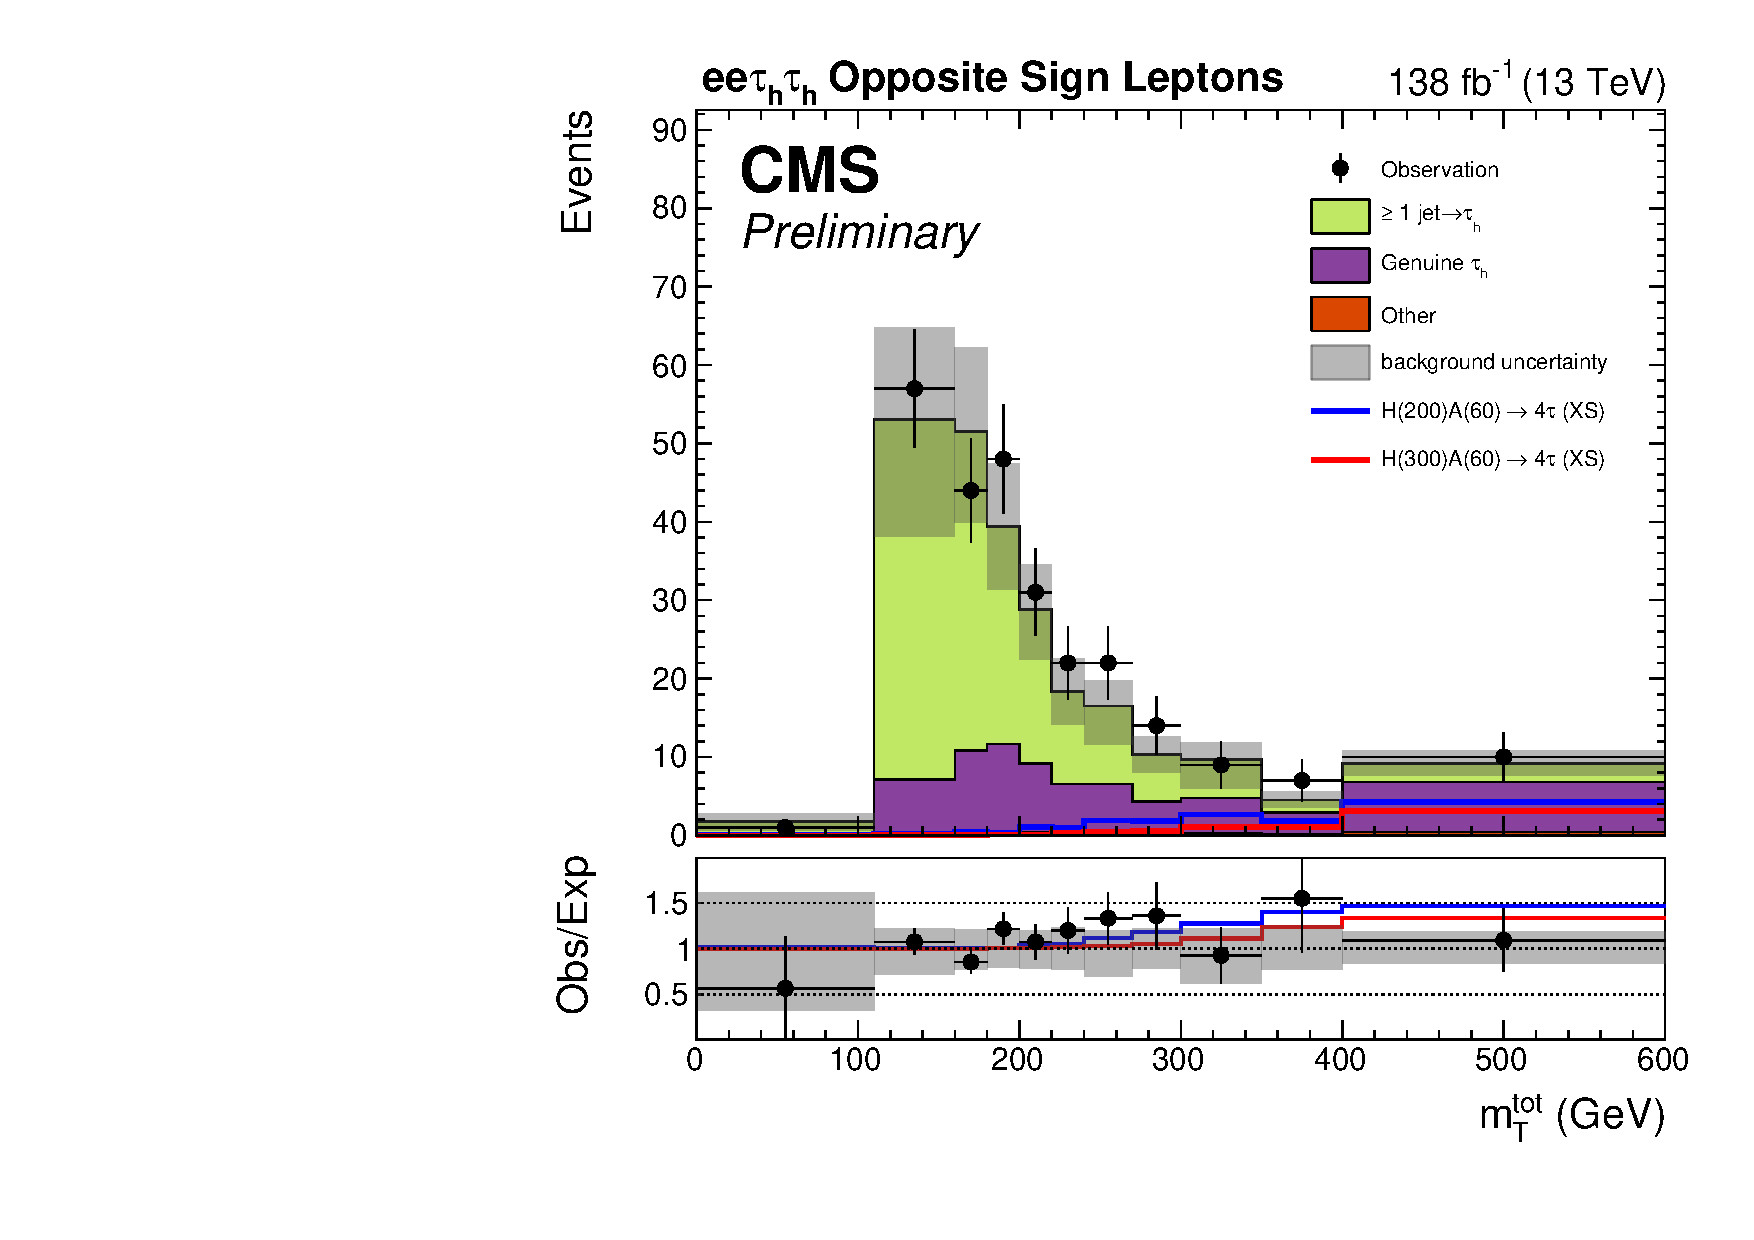
\includegraphics[width=0.4\textwidth]{Figures/mt_tot_signal_eett_z_control_nobtag_all.pdf}}
    \subfloat[]{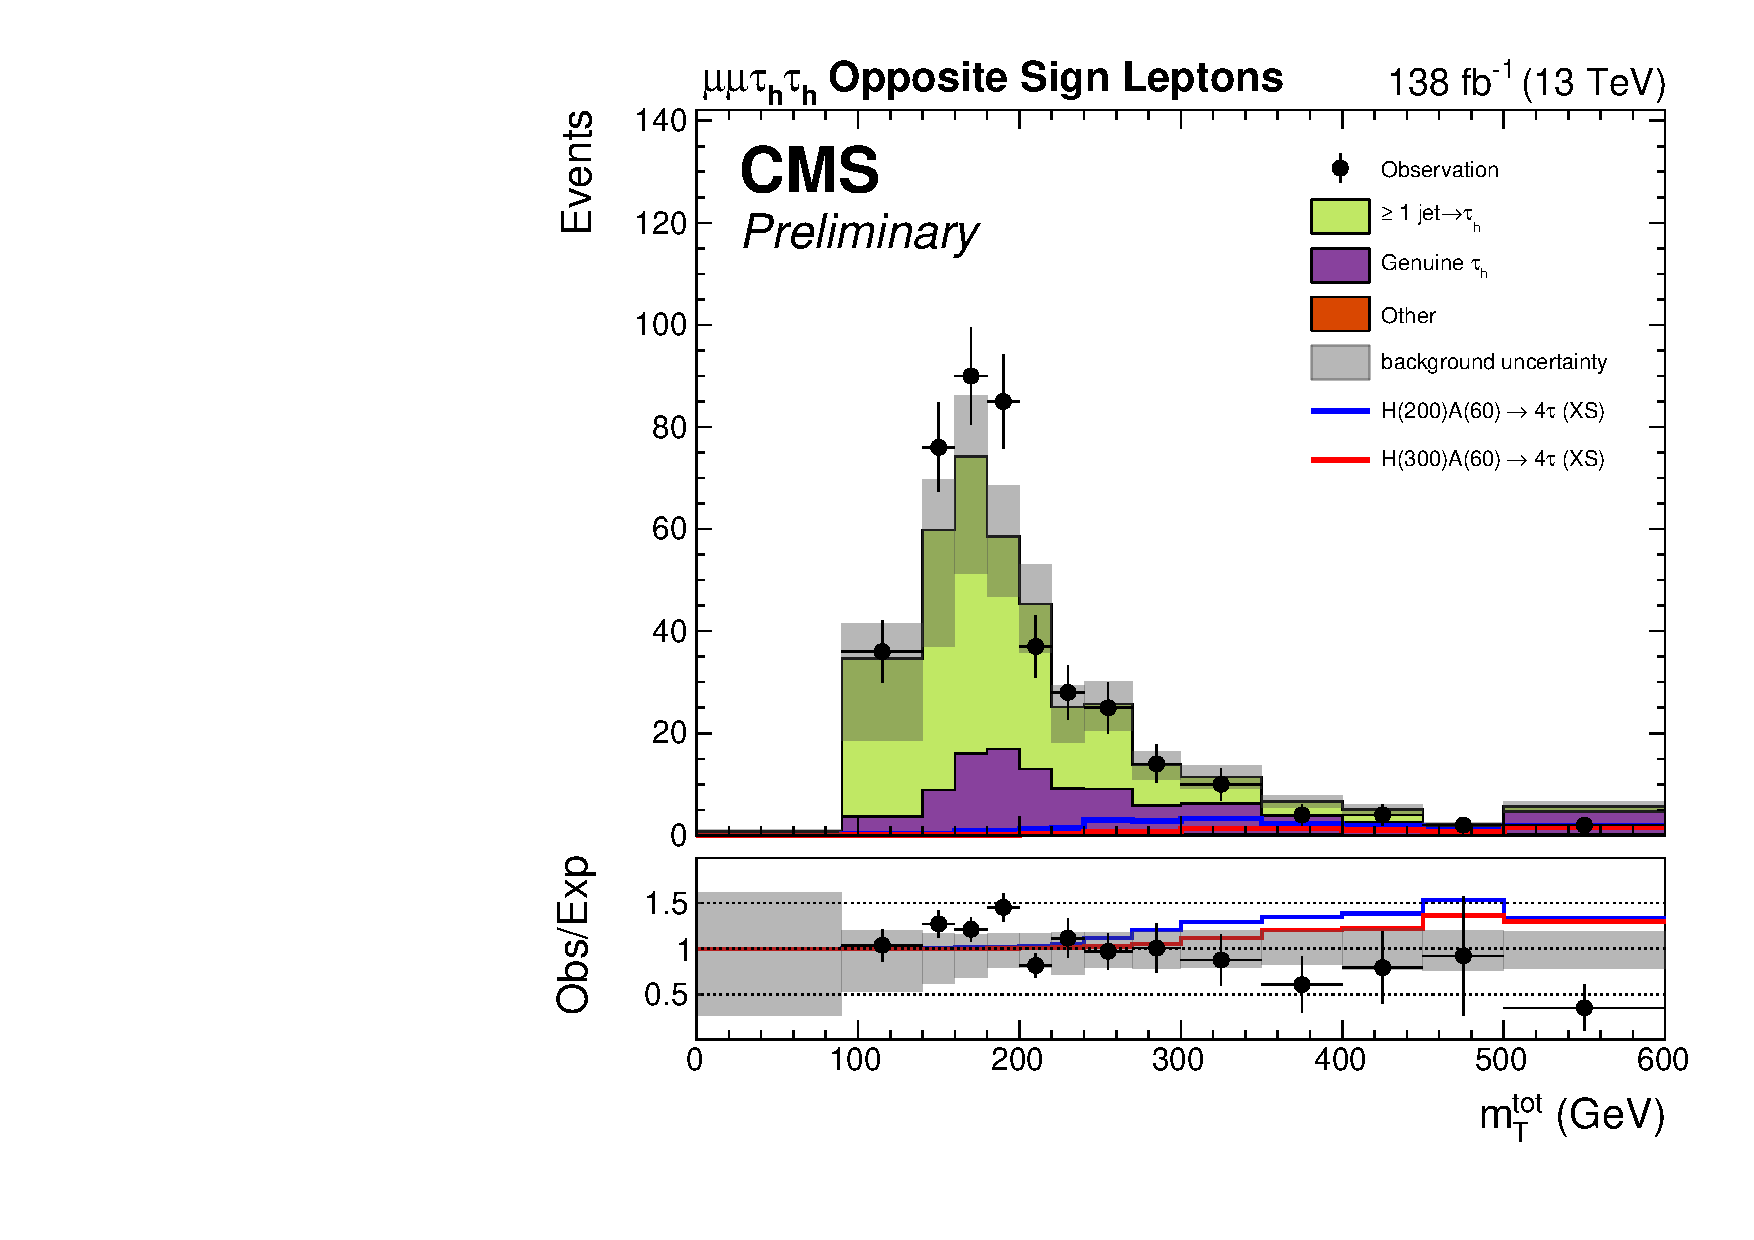
\includegraphics[width=0.4\textwidth]{Figures/mt_tot_signal_mmtt_z_control_nobtag_all.pdf}} \\
    \subfloat[]{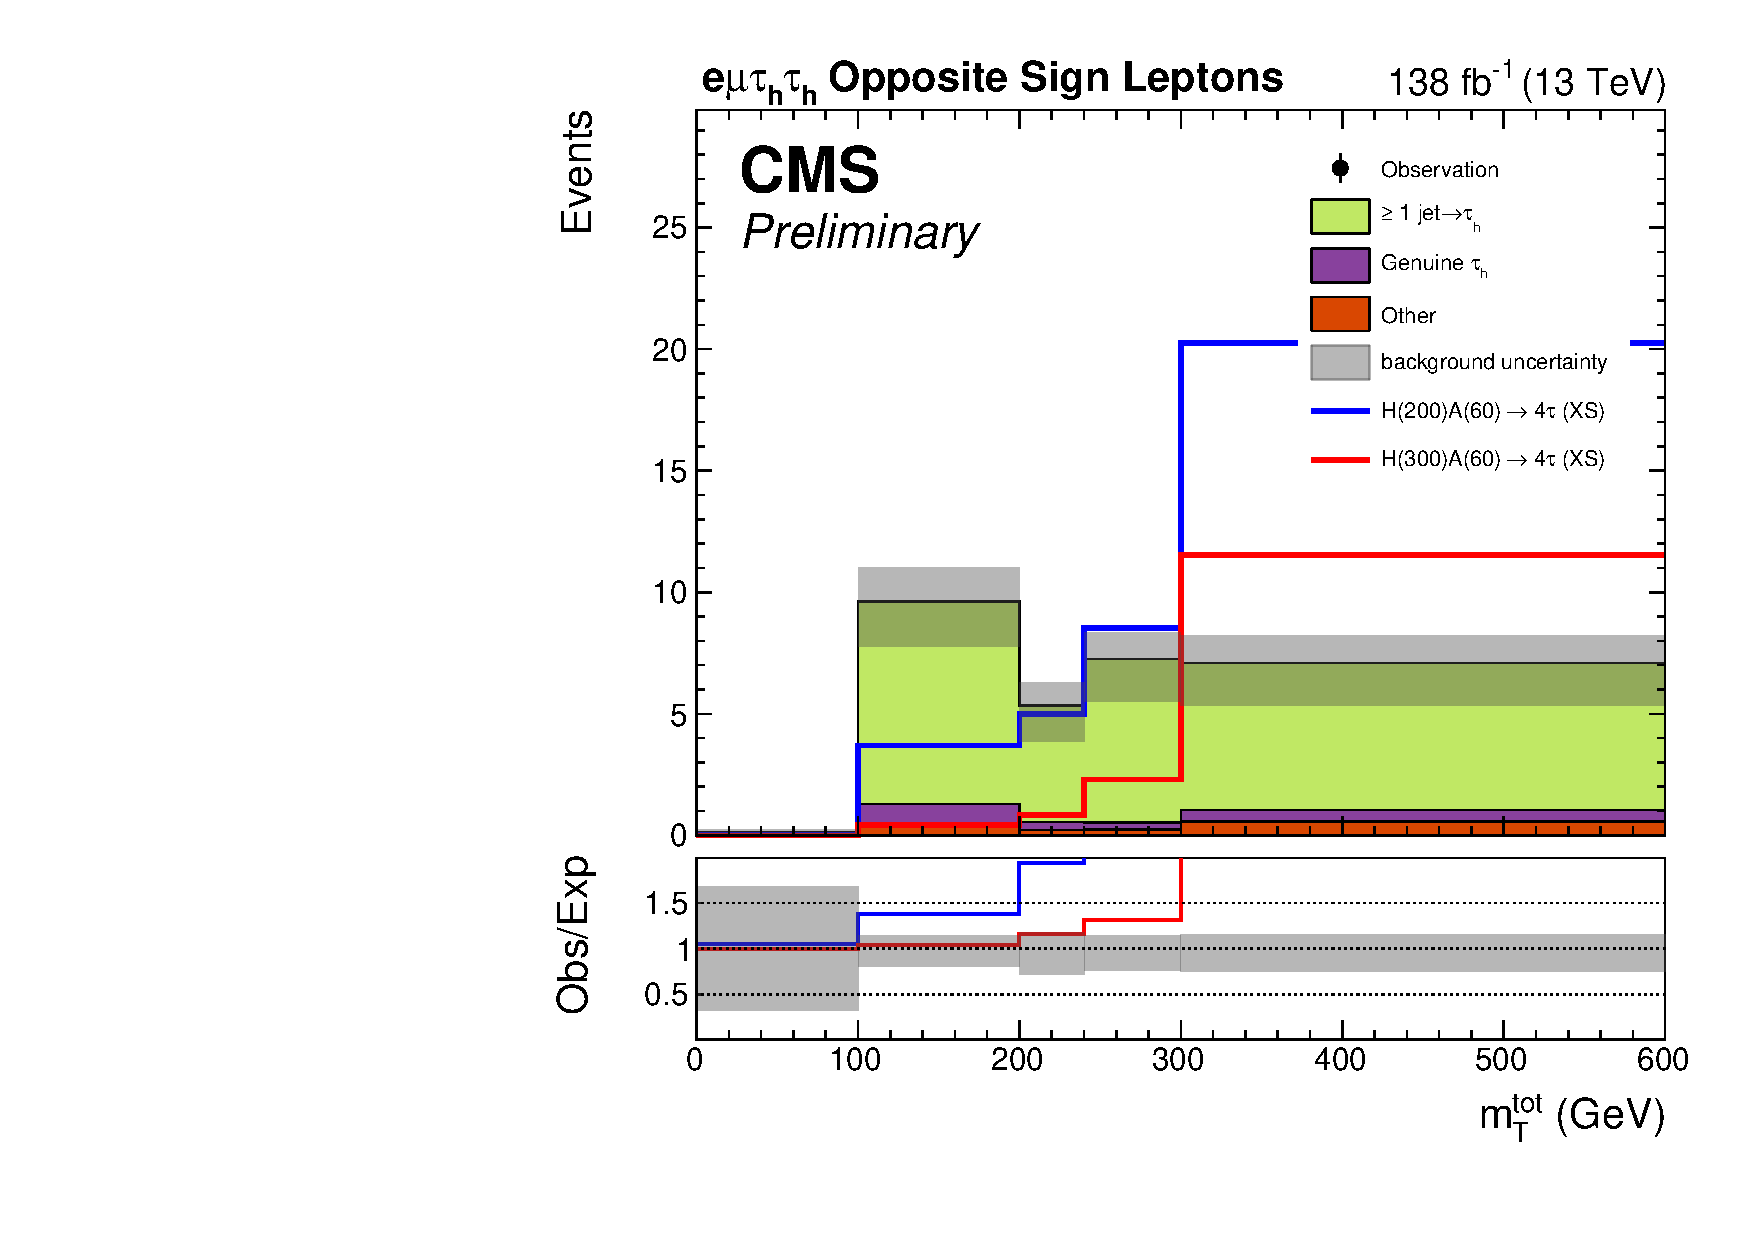
\includegraphics[width=0.4\textwidth]{Figures/mt_tot_signal_emtt_z_control_nobtag_all.pdf}}
    \subfloat[]{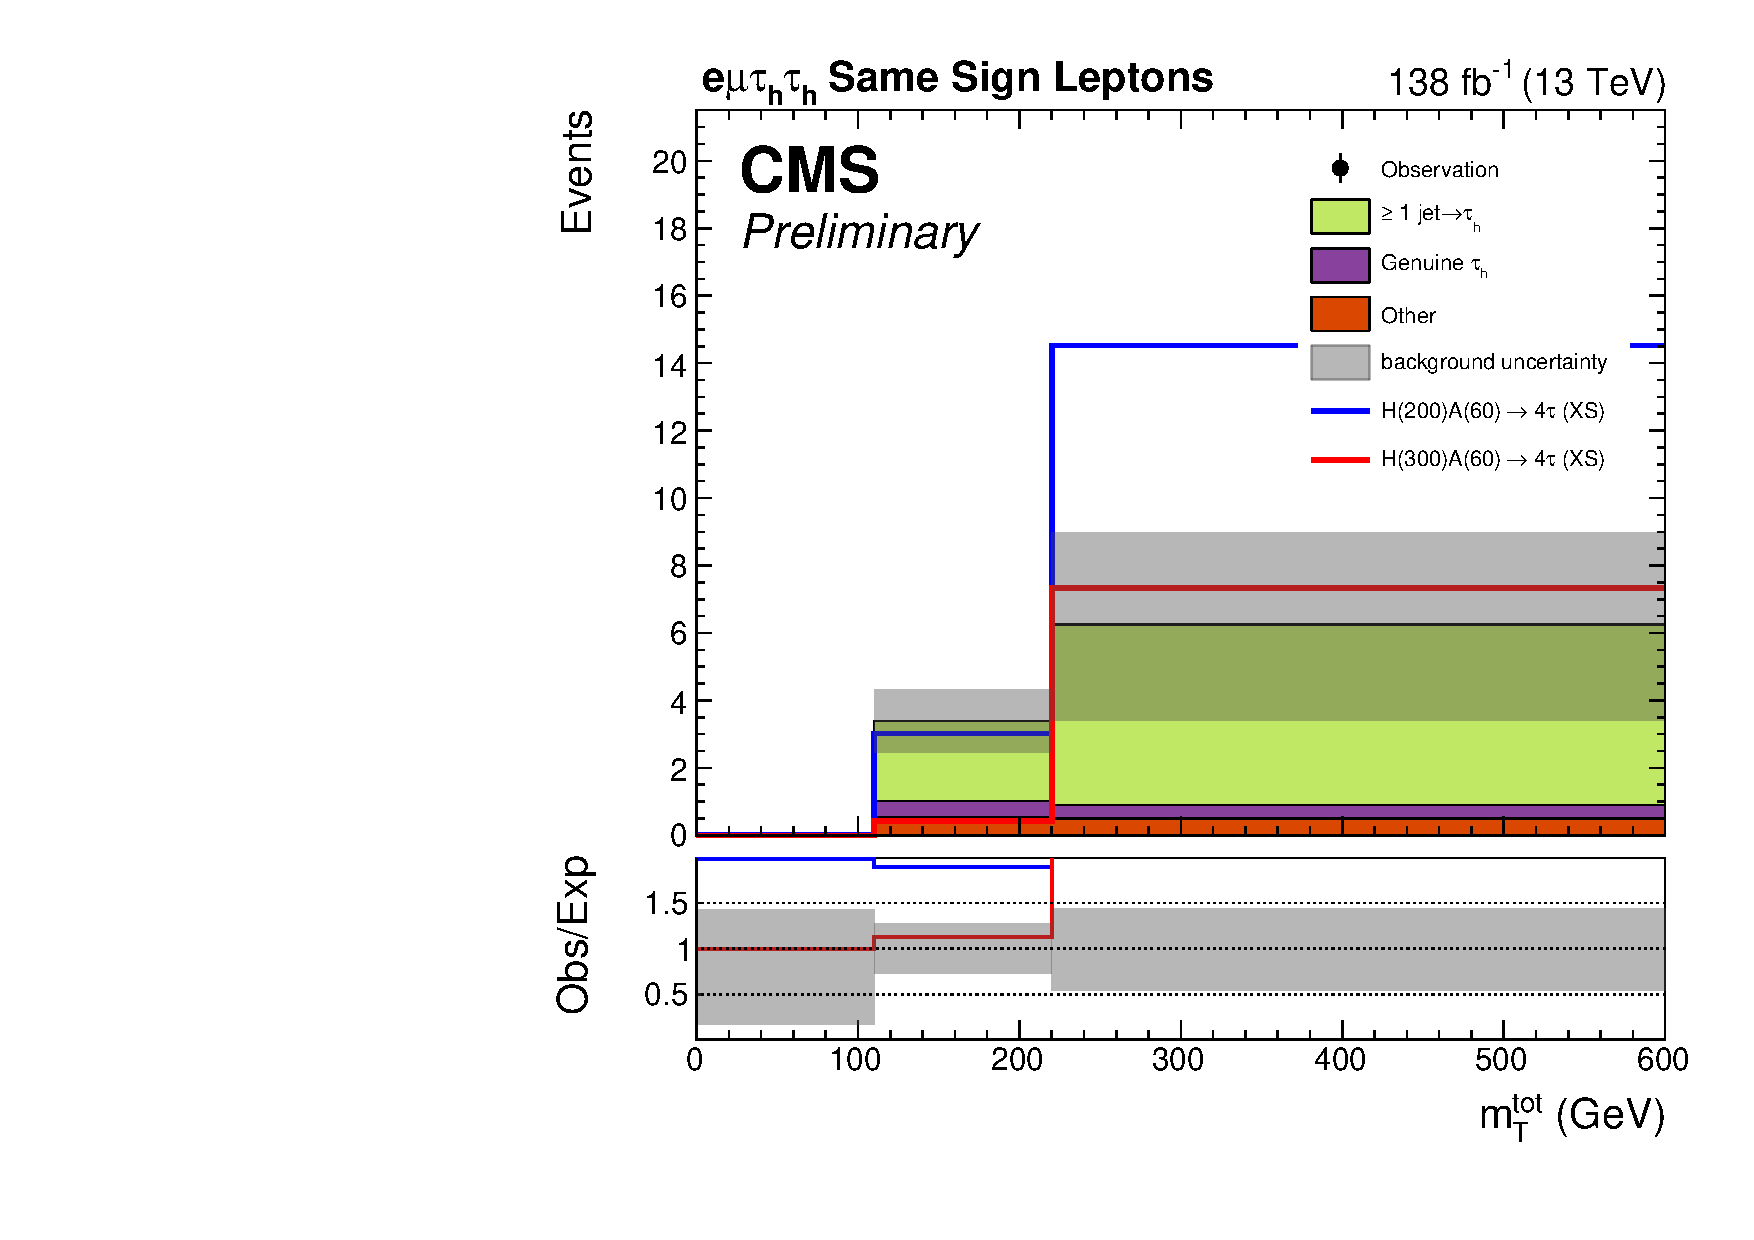
\includegraphics[width=0.4\textwidth]{Figures/mt_tot_signal_emtt_2l2t_sig_nobtag_all.pdf}} \\
    \subfloat[]{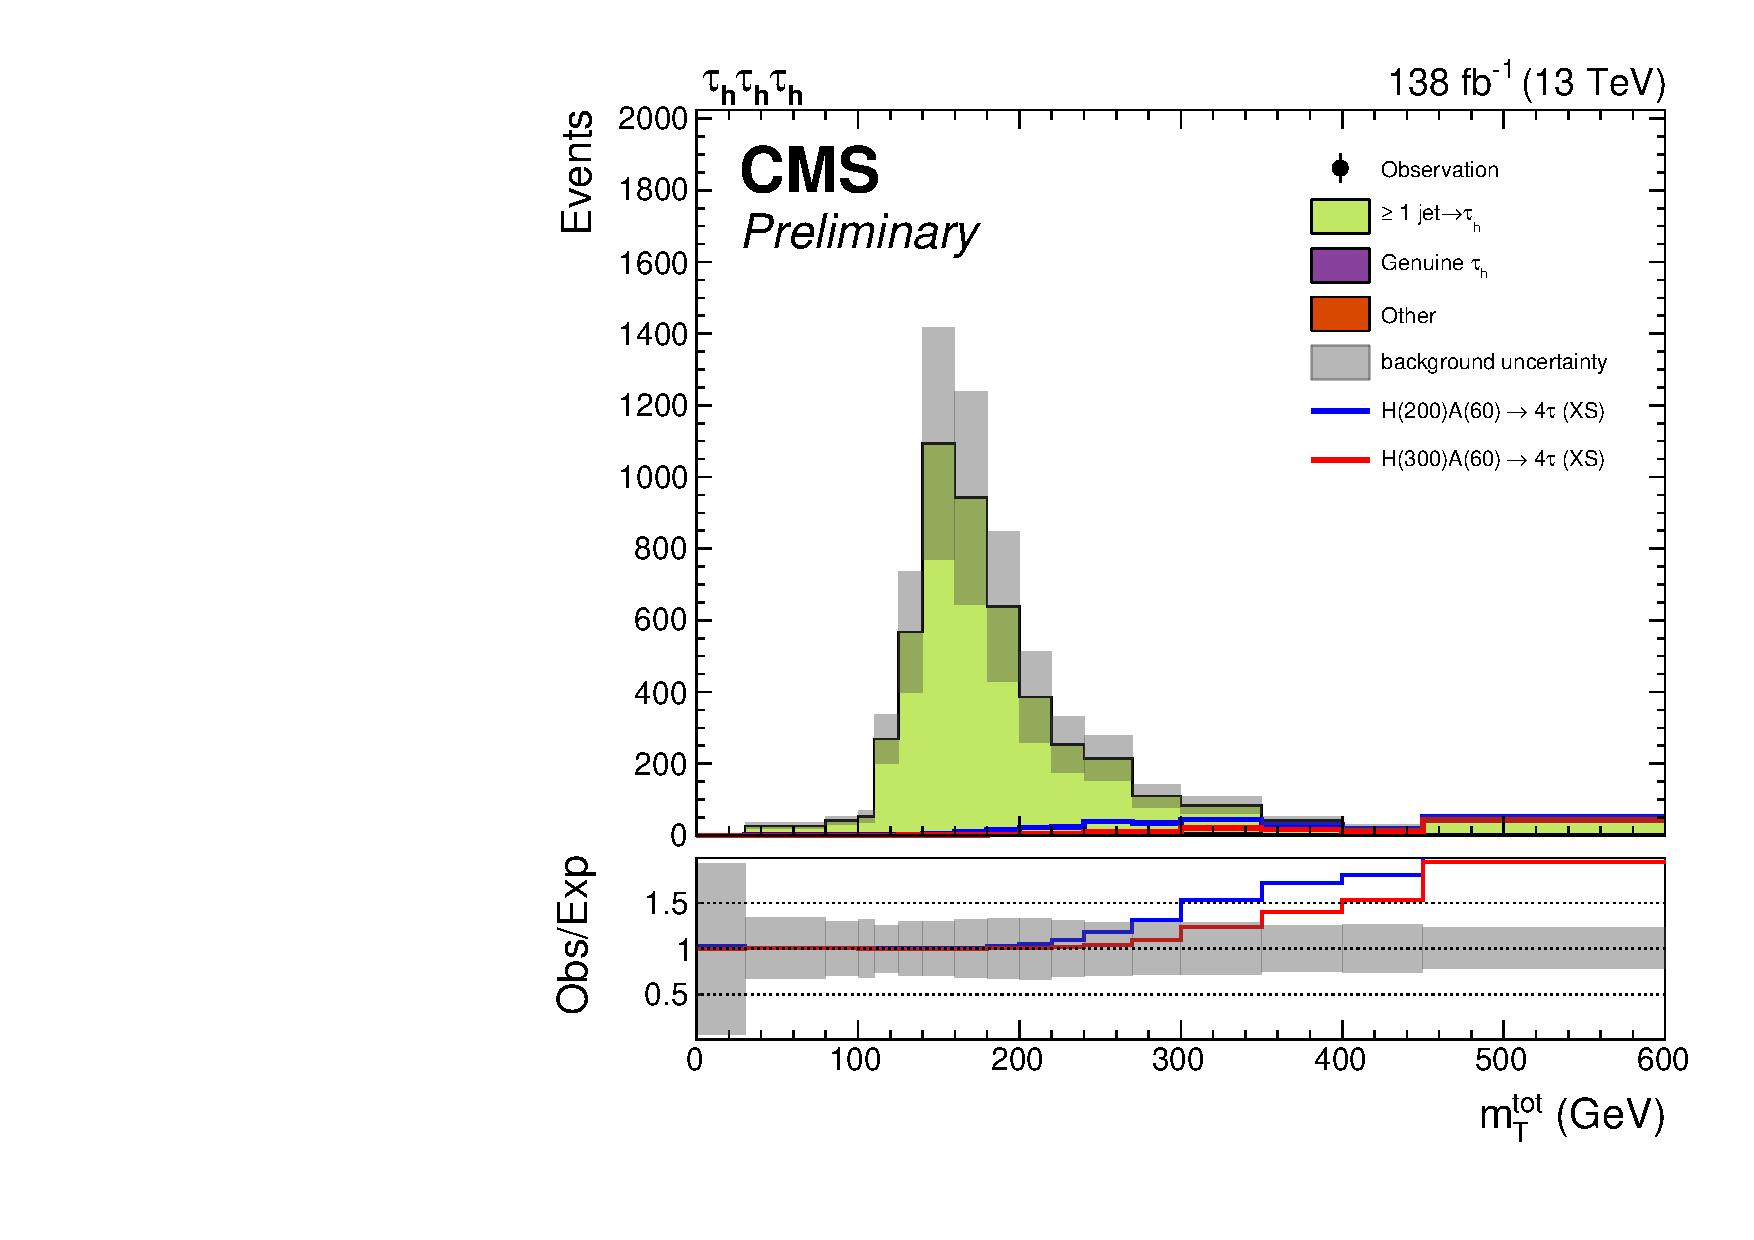
\includegraphics[width=0.4\textwidth]{Figures/mt_tot_signal_ttt_inclusive_all.pdf}}
\caption{Distributions of $m_{T}^\text{tot}$ in the $ee\tauhtauh$ OS Leptons (a) and $\mu\mu\tauhtauh$ OS Leptons (b), $e\mu\tauhtauh$ OS Leptons (c), $e\mu\tauhtauh$ SS Leptons (d) and $\tauh\tauh\tauh$ channel and categories. The solid histograms show the stacked background predictions after a background only fit to the data. The $m_{\phi}=100$ GeV and $m_{A}=100$ GeV signal is also shown for illustrative purposes.}
\label{fig:4tau_postfit}
\end{figure}

\begin{figure}[!hbtp]
\centering
    \subfloat[]{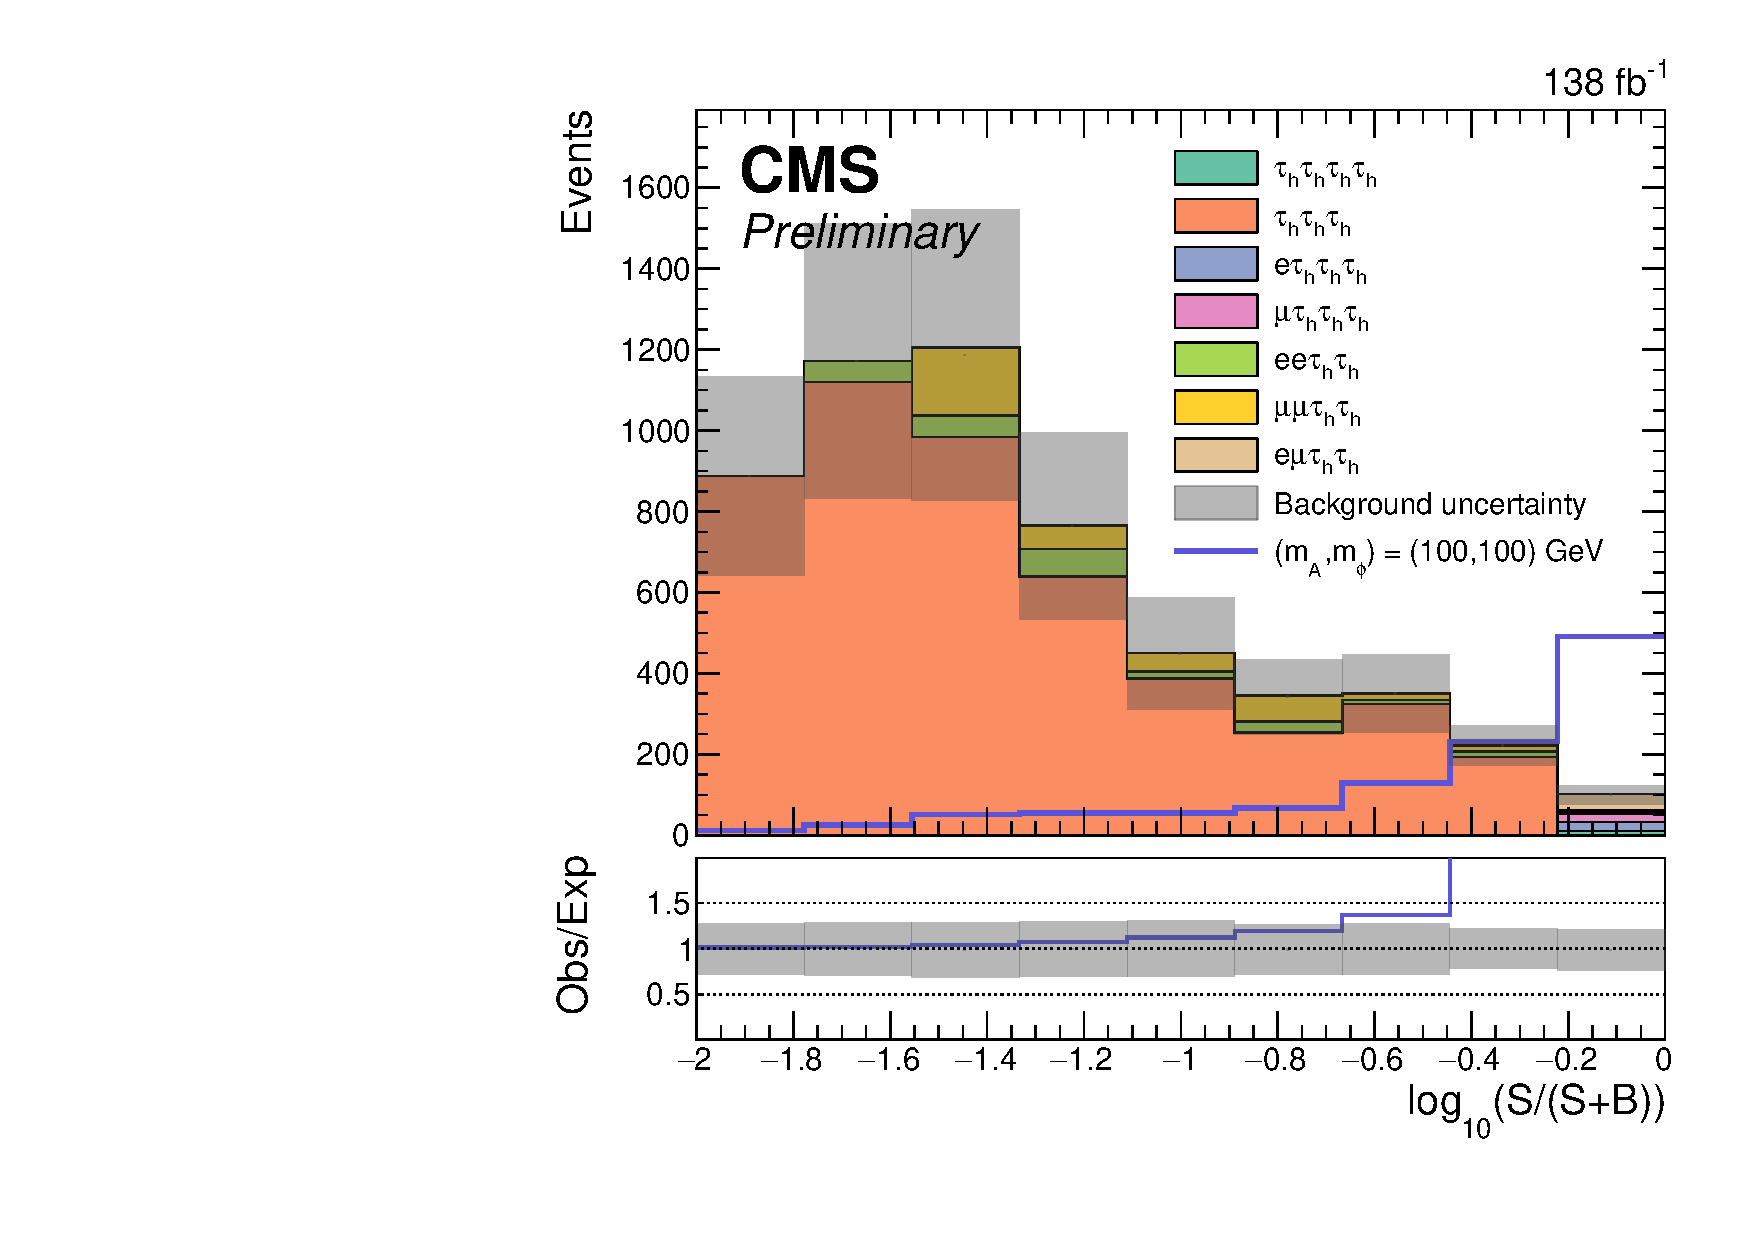
\includegraphics[width=0.45\textwidth]{Figures/soversplusb_plot_phi100A100.pdf}}
    \subfloat[]{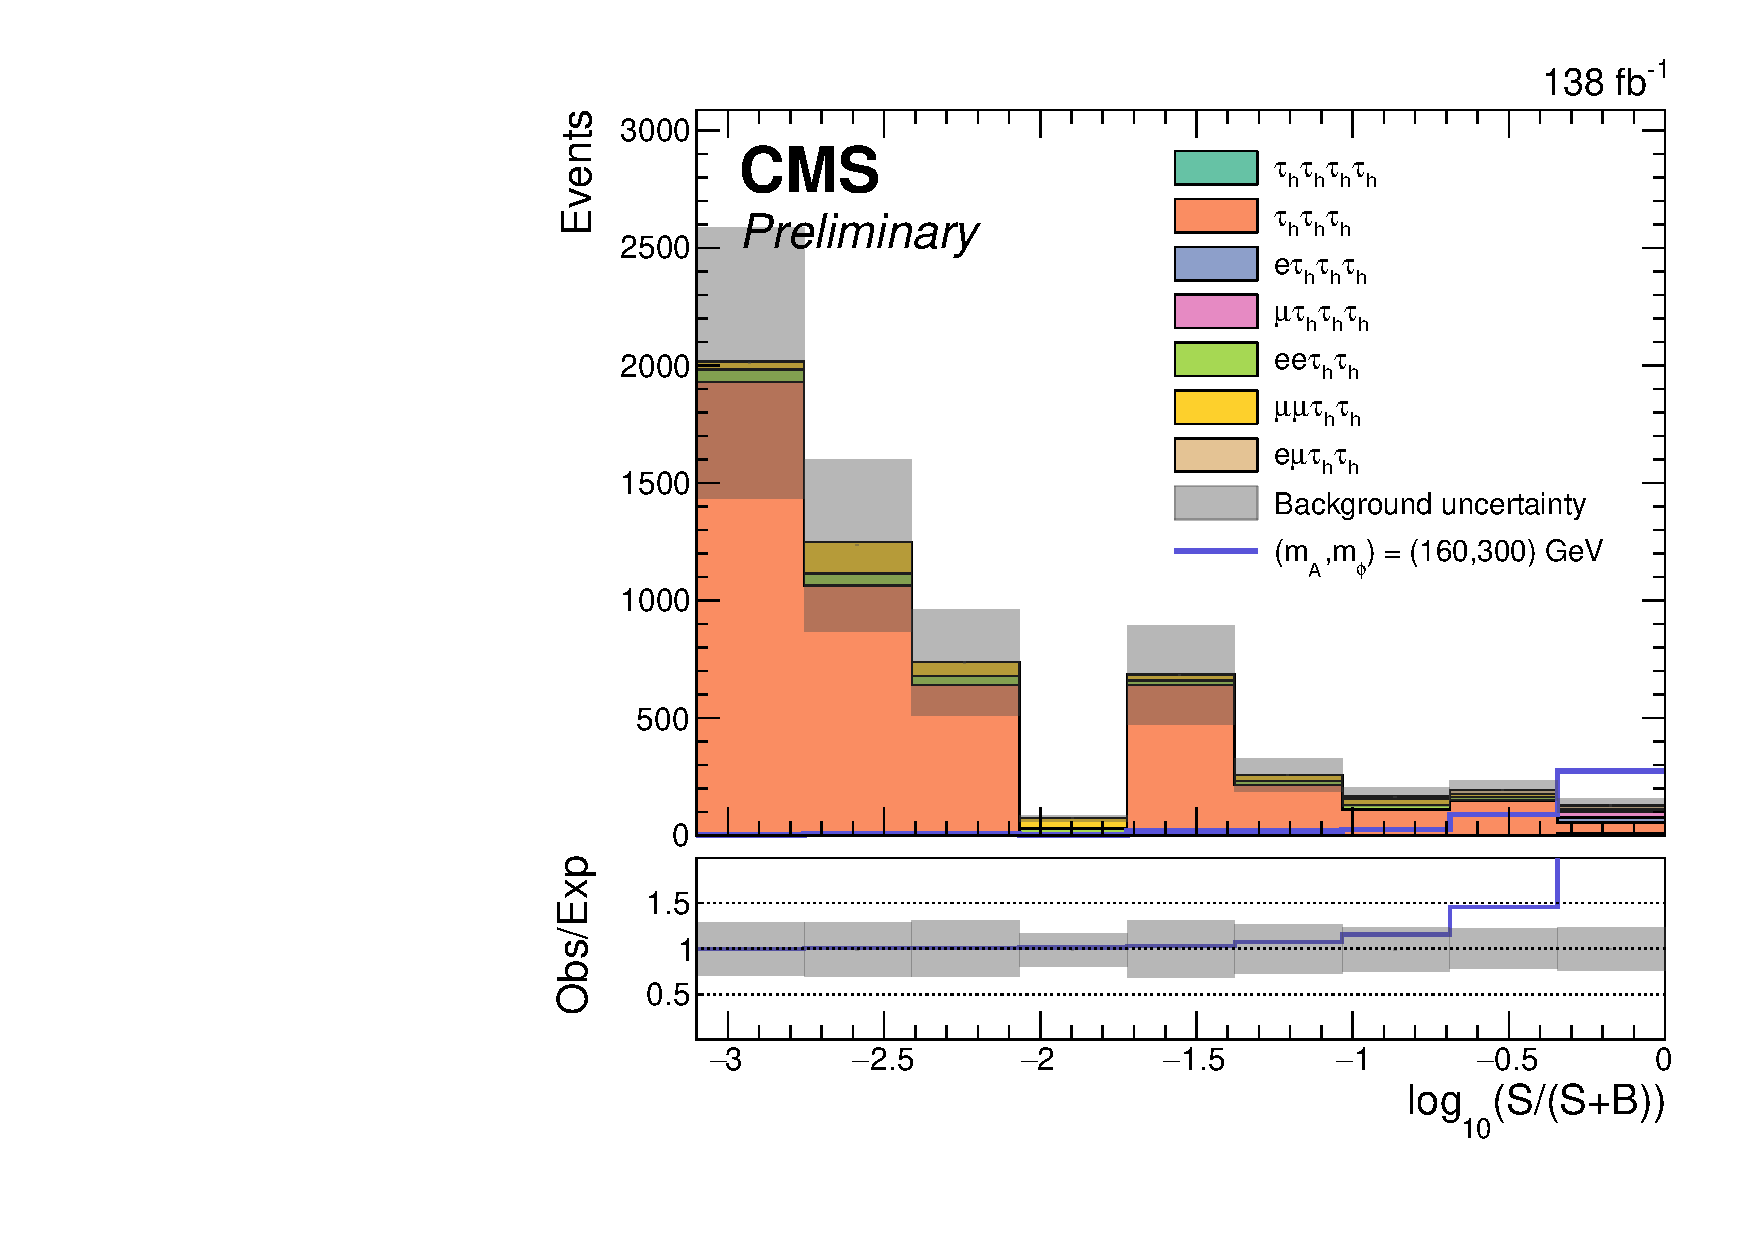
\includegraphics[width=0.45\textwidth]{Figures/soversplusb_plot_phi300A160.pdf}} 
\caption{Distributions of events with respect to the $\log_{10}(S/(S+B))$ of all analysis category bins fit for two signal scenarios: $m_{\phi}=100$ GeV and $m_{A}=100$ GeV and $m_{\phi}=160$ GeV and $m_{A}=160$ GeV. The solid histograms show the stacked background predictions after a background only fit to the data. The signal model considered is displayed with a solid line. }
\label{fig:4tau_soversplusb}
\end{figure}

\section{Model Independent Results}

\begin{figure}[!hbtp]
\centering
    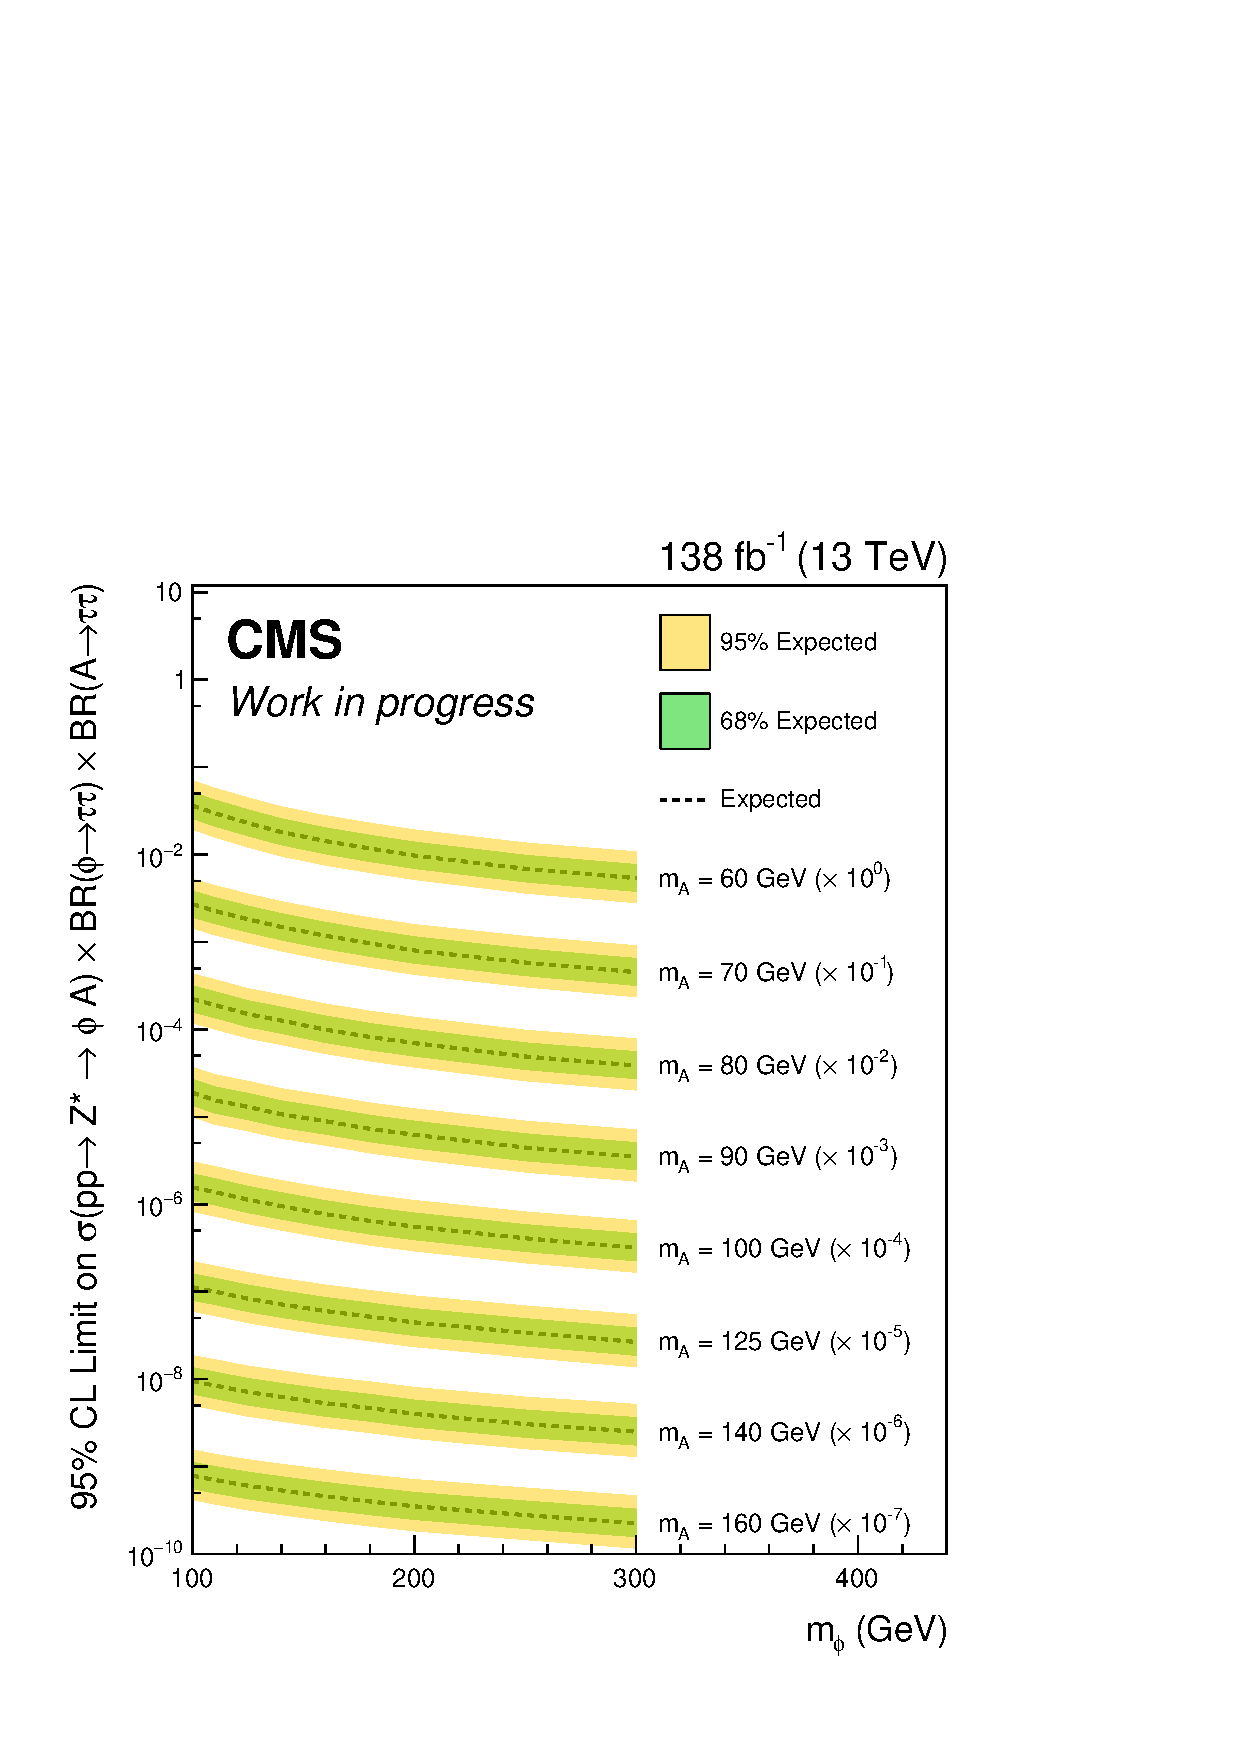
\includegraphics[width=0.9\textwidth]{Figures/model_independent_limit_all.pdf}
\caption{Expected (dashed line) and observed (solid line and dots) 95\% CL upper limits on the product of the cross sections and branching fractions for the decay of both additional Higgs bosons into $\tau$ leptons. Different $m_{A}$ hypotheses are scaled by different orders of magnitudes (written on plot) in order to make mass points distinguishable. The dark green and bright yellow bands indicate the central 68\% and 95\% intervals for the expected exclusion limit.}
\label{fig:4tau_mi}
\end{figure}

\begin{figure}[!hbtp]
\centering
    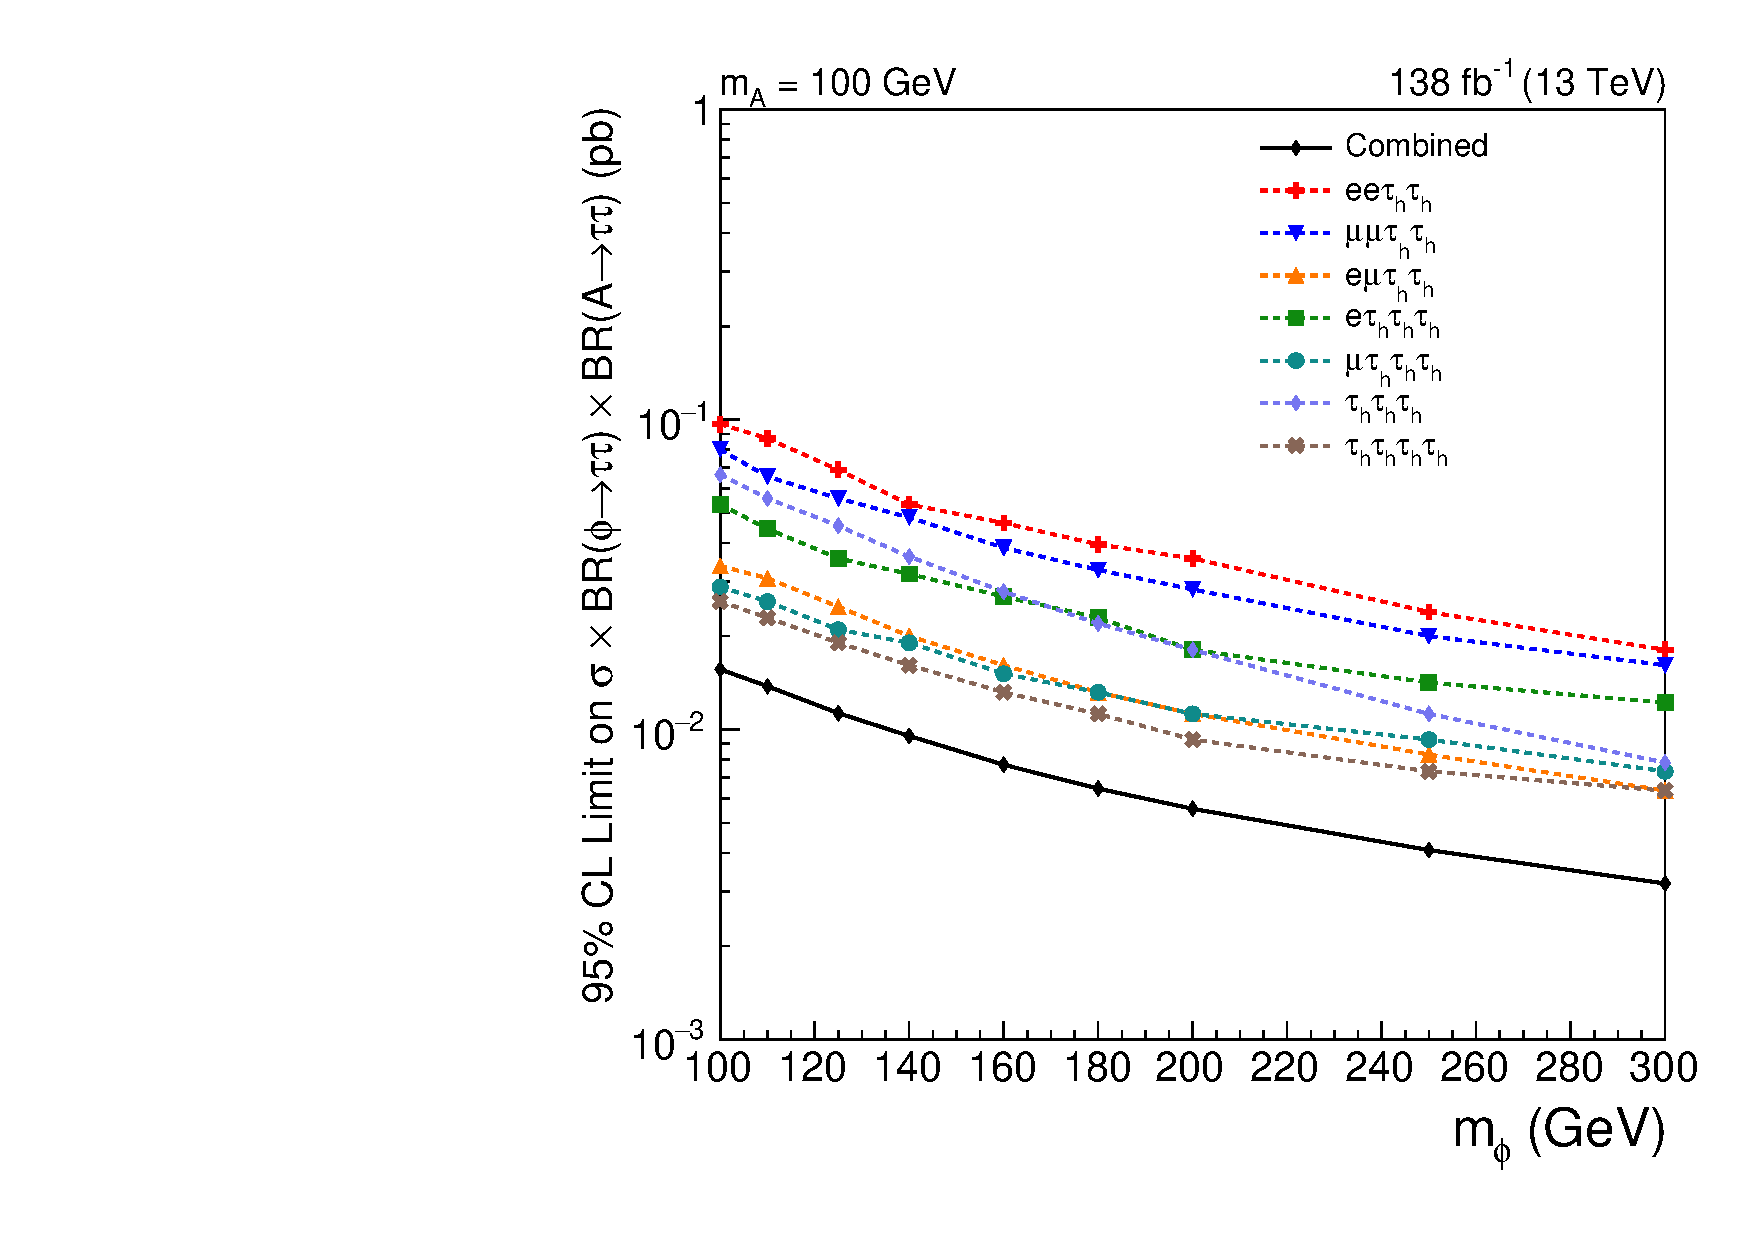
\includegraphics[width=0.6\textwidth]{Figures/limit_comparison_4tau.pdf}
\caption{Comparison of the expected 95\% CL upper limits on the product of the cross sections and branching fractions for the decay into $\tau$ leptons, split by the $\tau\tau\tau\tau$ decay products fit individually.}
\label{fig:4tau_limit_comparison}
\end{figure}

\begin{figure}[!hbtp]
\centering
    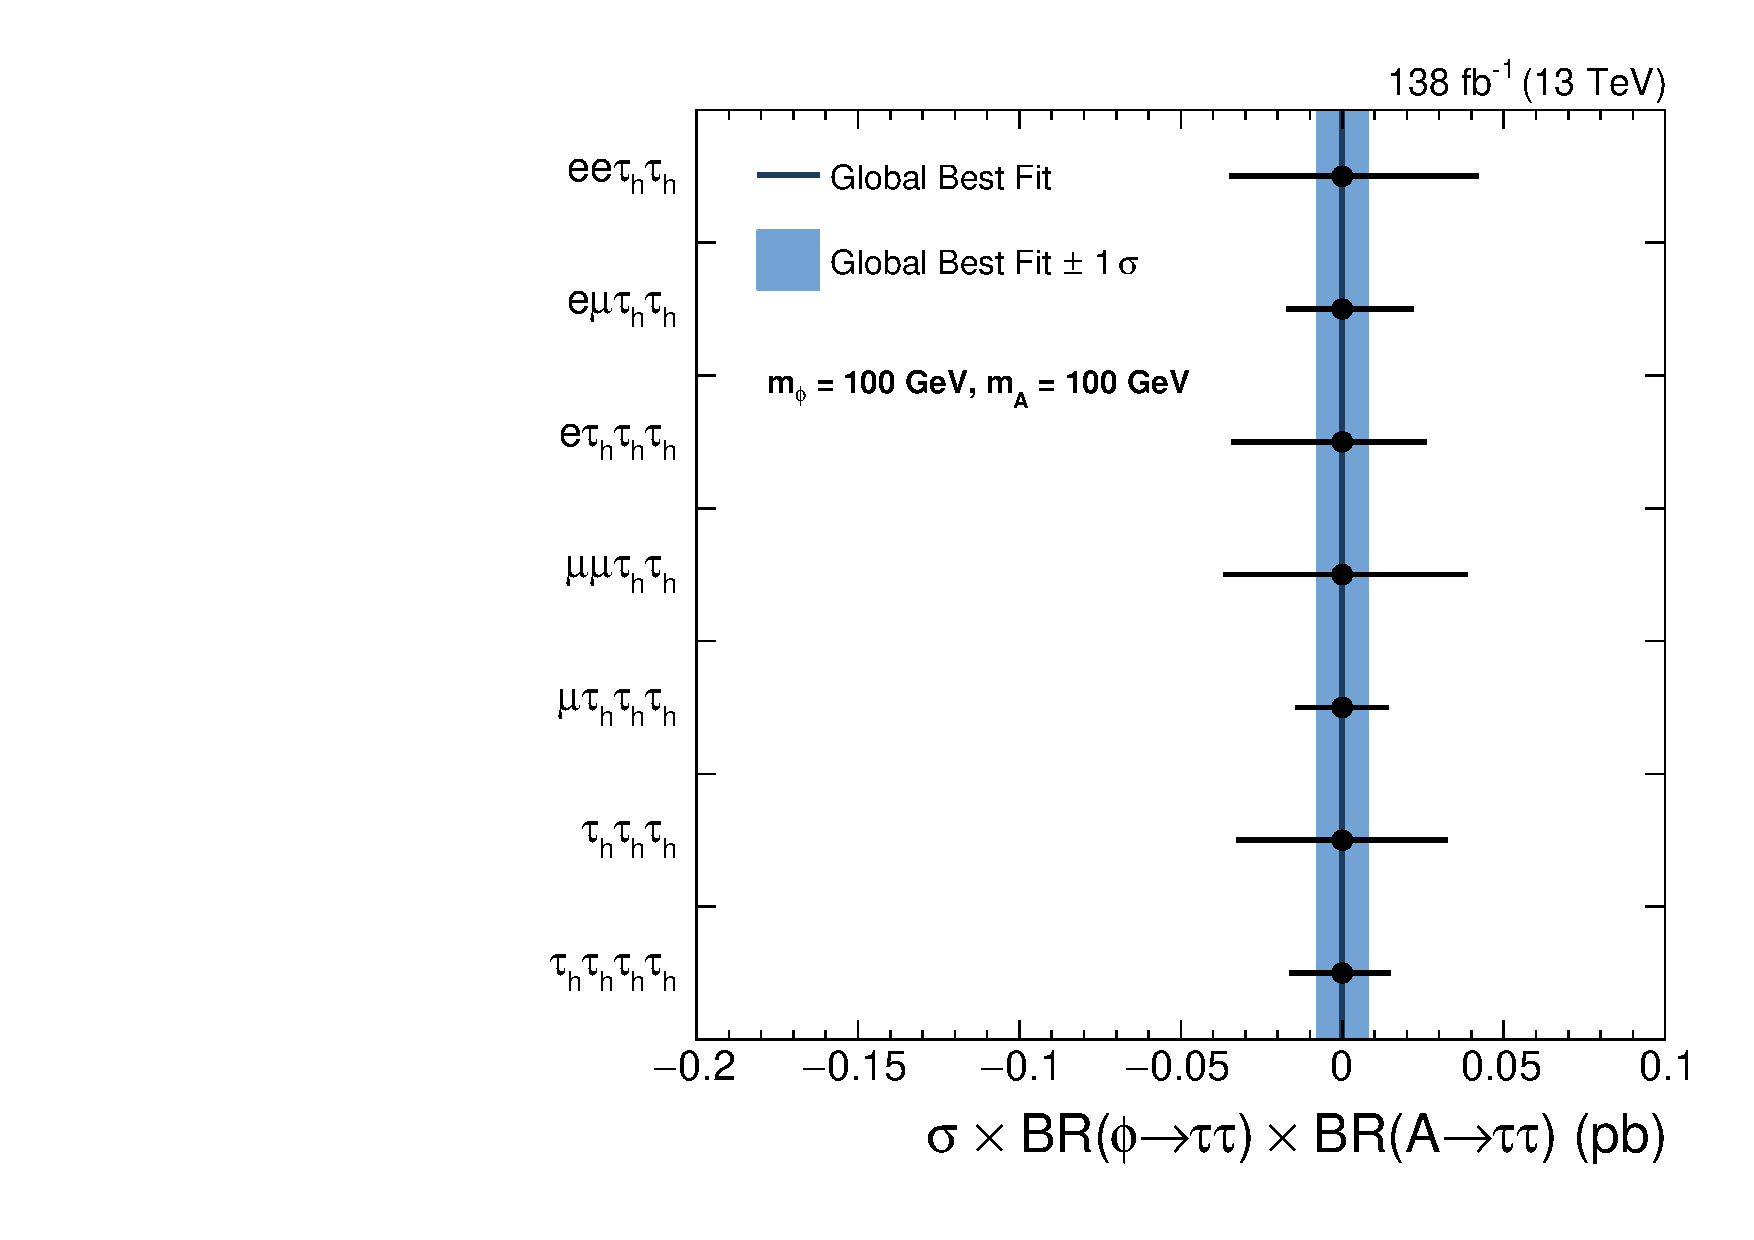
\includegraphics[width=0.6\textwidth]{Figures/ChannelCompatibilityCheck_FitResults_mphi100mA100_channel.pdf}
\caption{Compatibility plots for the $m_{A}=100$ GeV and $m_{\phi}=100$ GeV mass scenario in analysis decay channels. In each case the fitted signal strength is decoupled in the bin shown on the plot.}
\label{fig:4tau_ccc}
\end{figure}

\section{Model Dependent Limits}

\begin{figure}[!hbtp]
\centering
    \subfloat[]{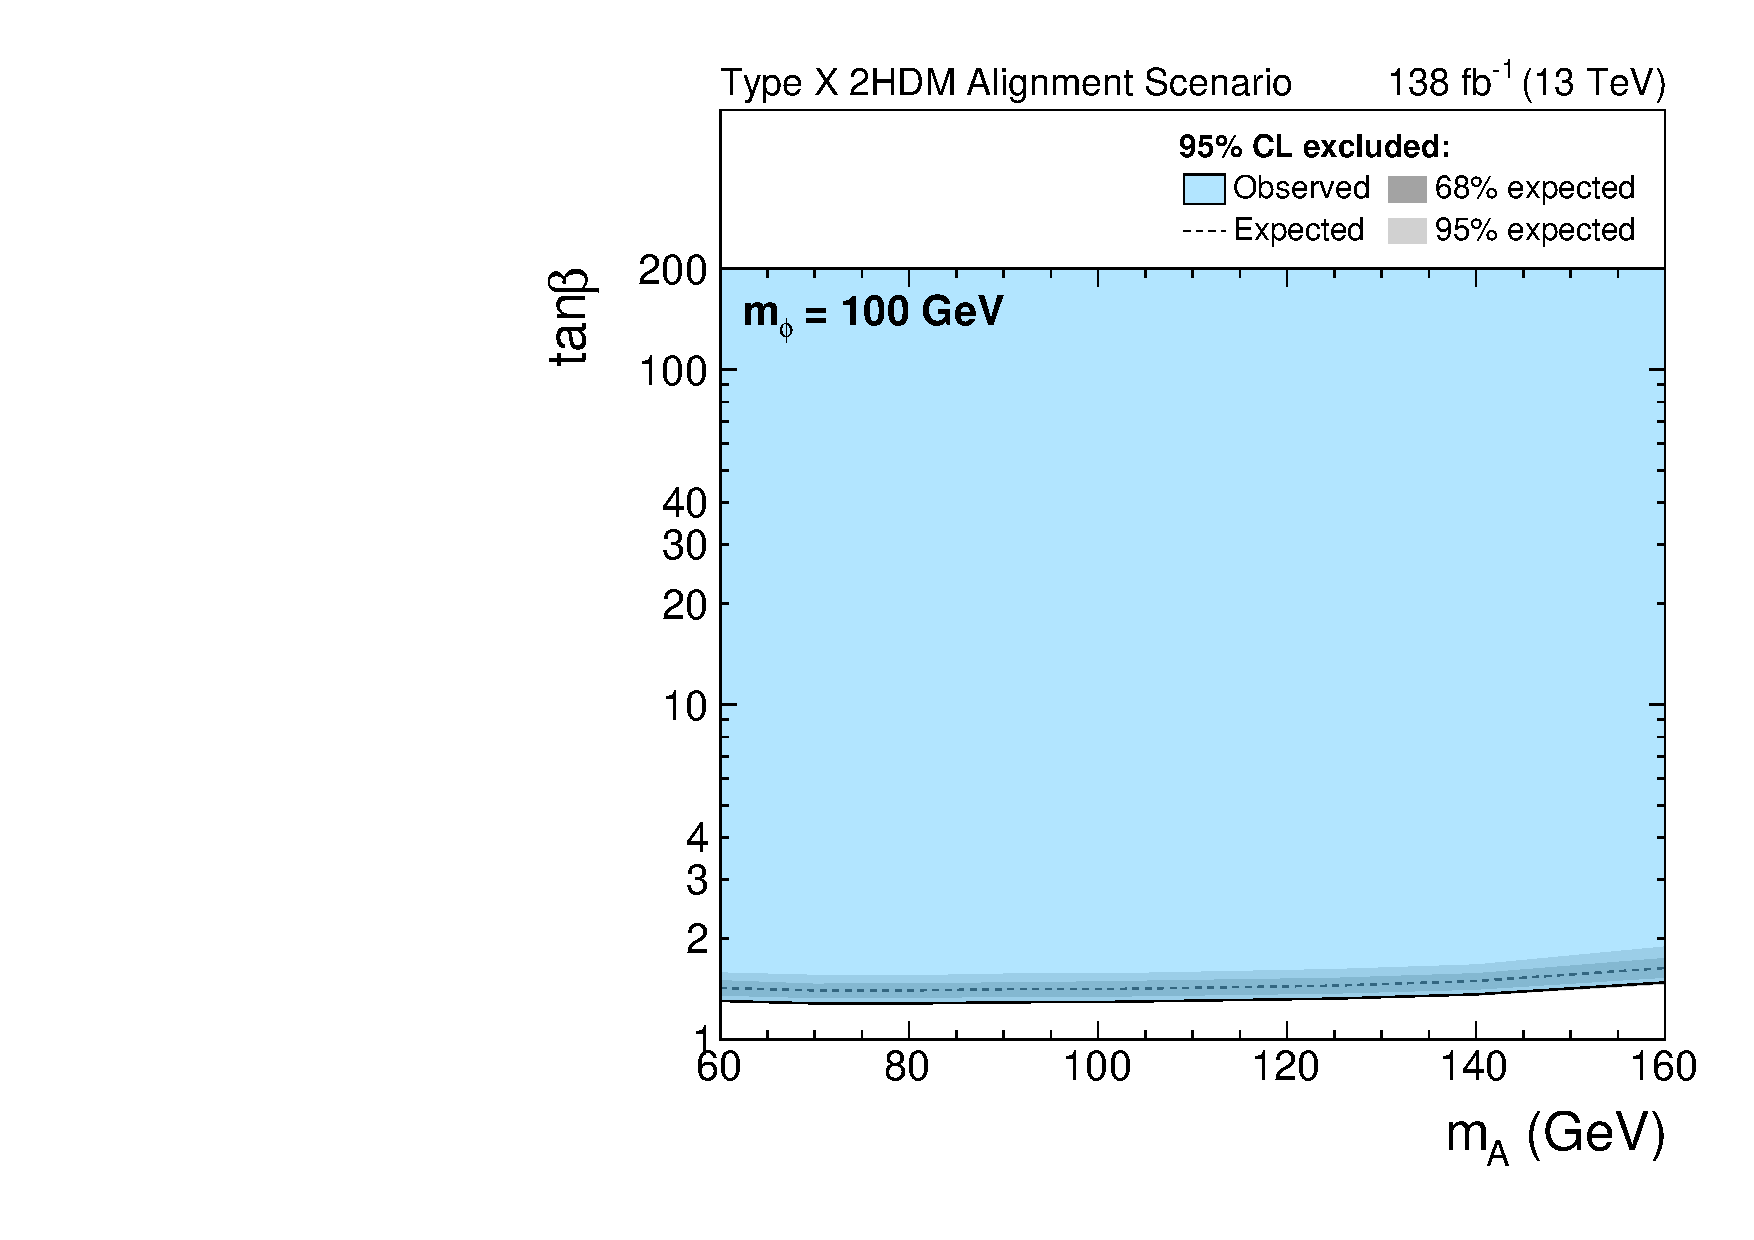
\includegraphics[width=0.65\textwidth]{Figures/md_mphi100.pdf}} \\
    \subfloat[]{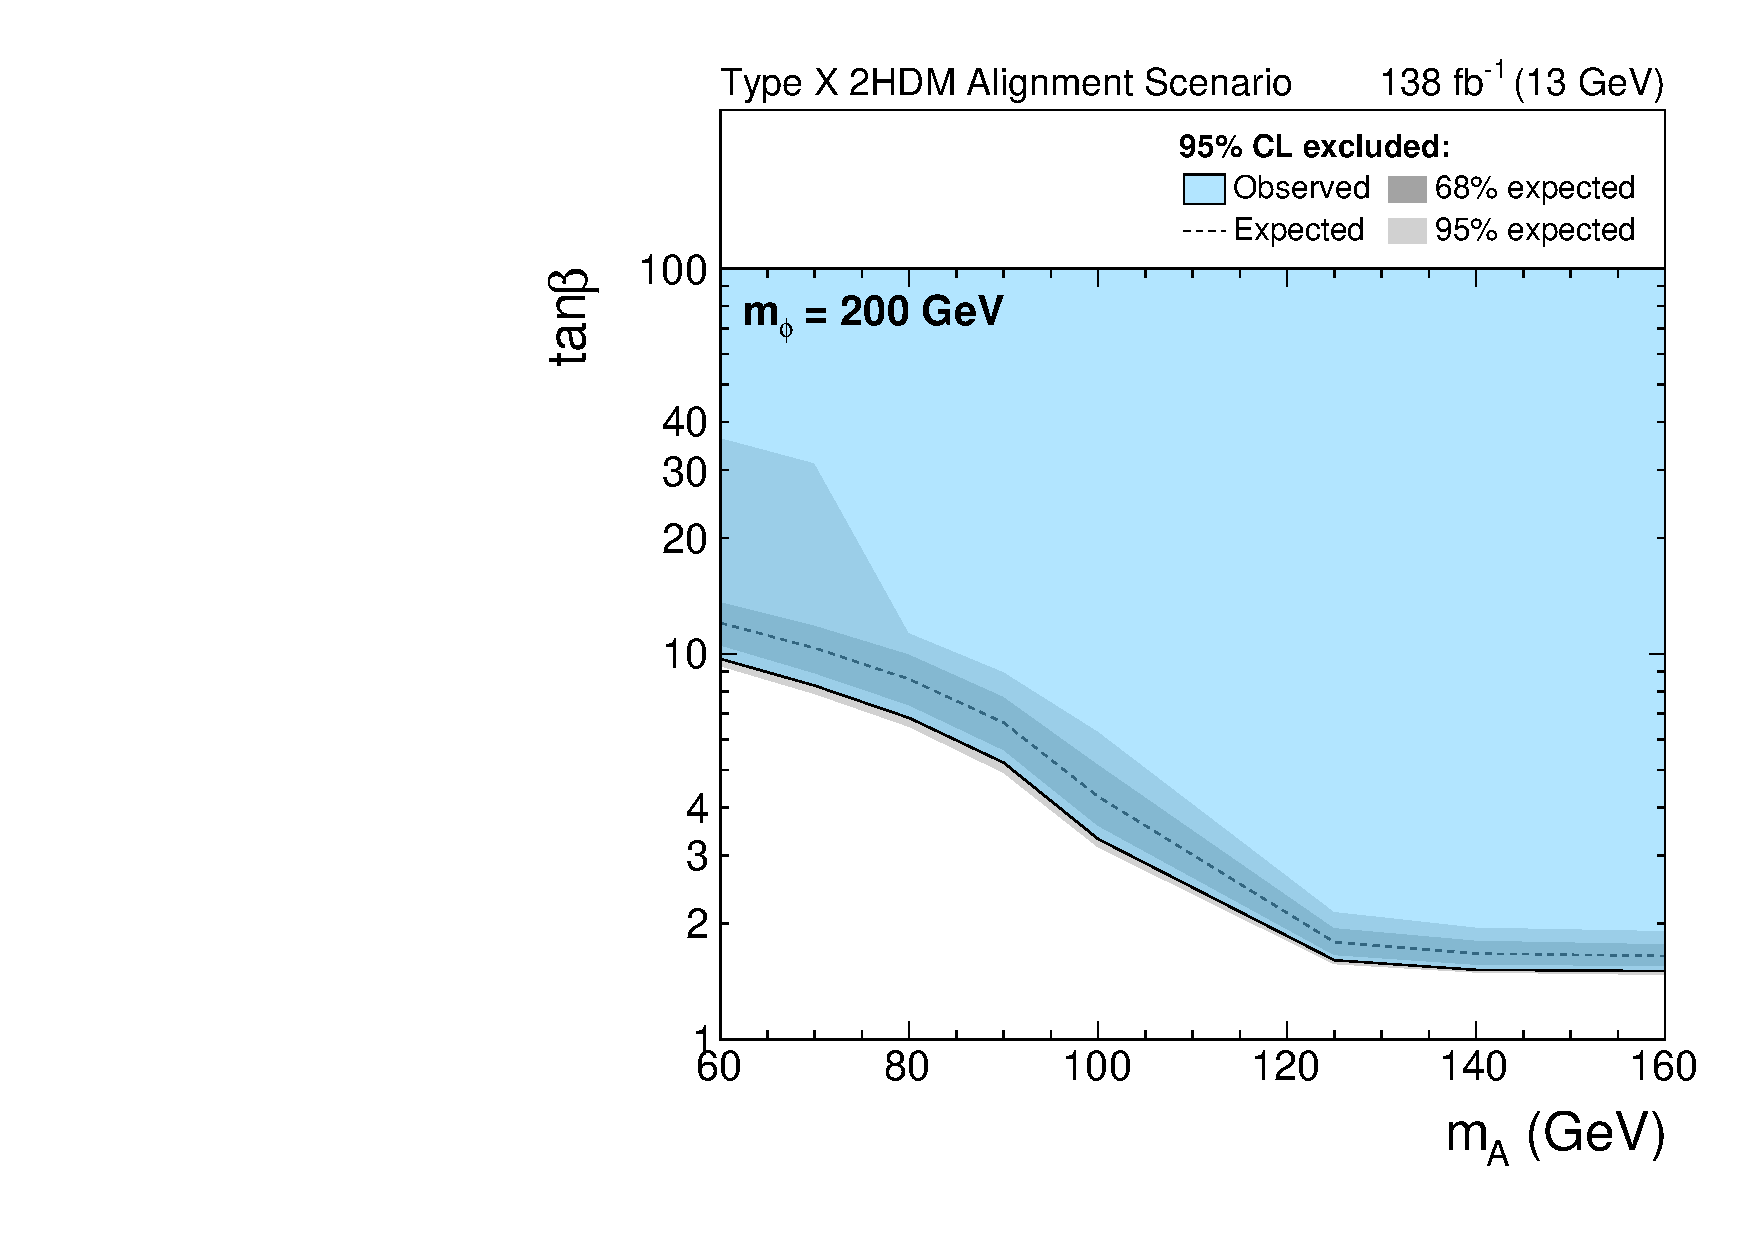
\includegraphics[width=0.65\textwidth]{Figures/md_mphi200.pdf}} 
\caption{Expected and observed 95\% CL exclusion contours on the $m_{A}$-$\tan\beta$ phase space in the type X 2HDM alignment scenario for $m_{\phi}$ scenarios of 100 GeV (a) and 200 GeV (b). The exclusion limit only on background expectation is shown as a dashed black line, the dark and bright grey bands show the 68\% and 95\% intervals of the expected exclusion and the observed exclusion contour is shown by the blue area.}
\label{fig:4tau_md}
\end{figure}

\begin{figure}[!hbtp]
\centering
    \subfloat[]{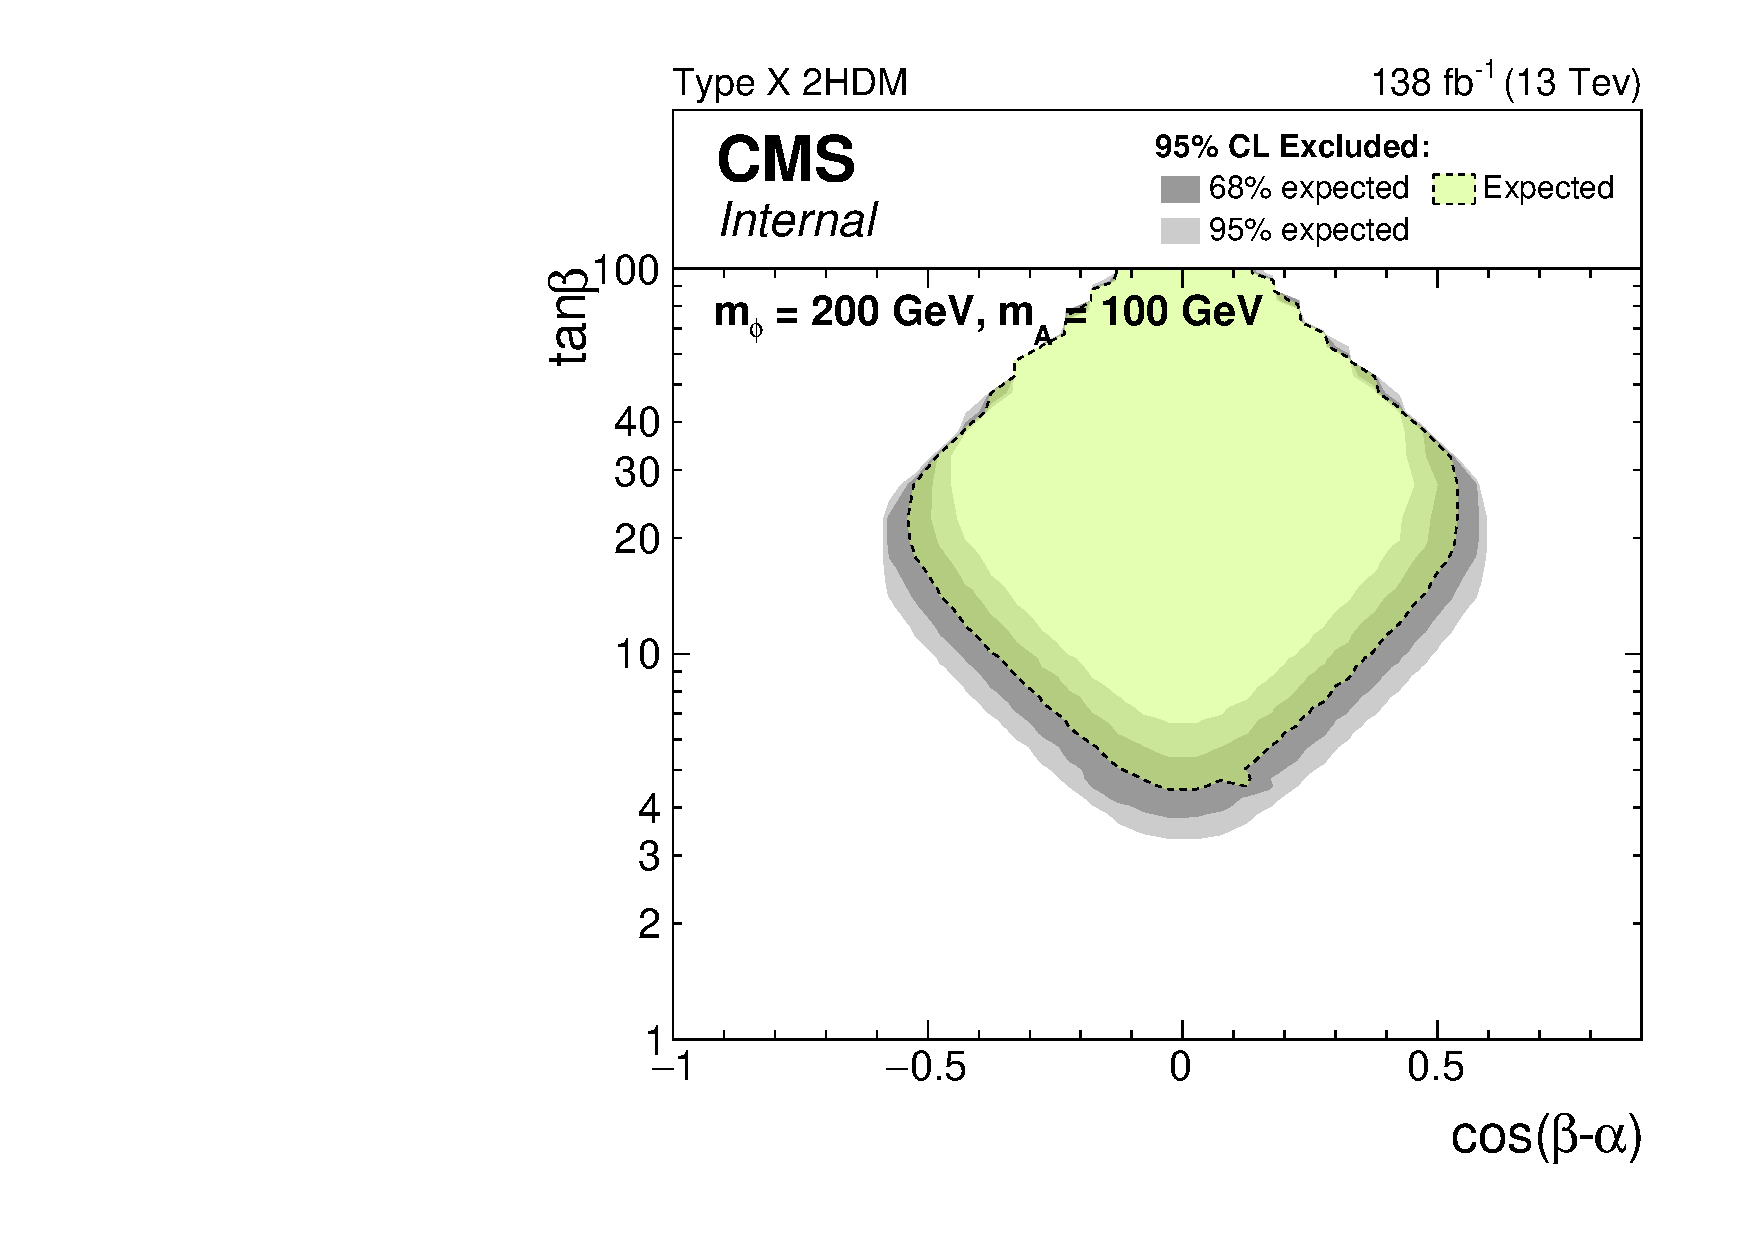
\includegraphics[width=0.65\textwidth]{Figures/csbma_phi200A100.pdf}} \\
    \subfloat[]{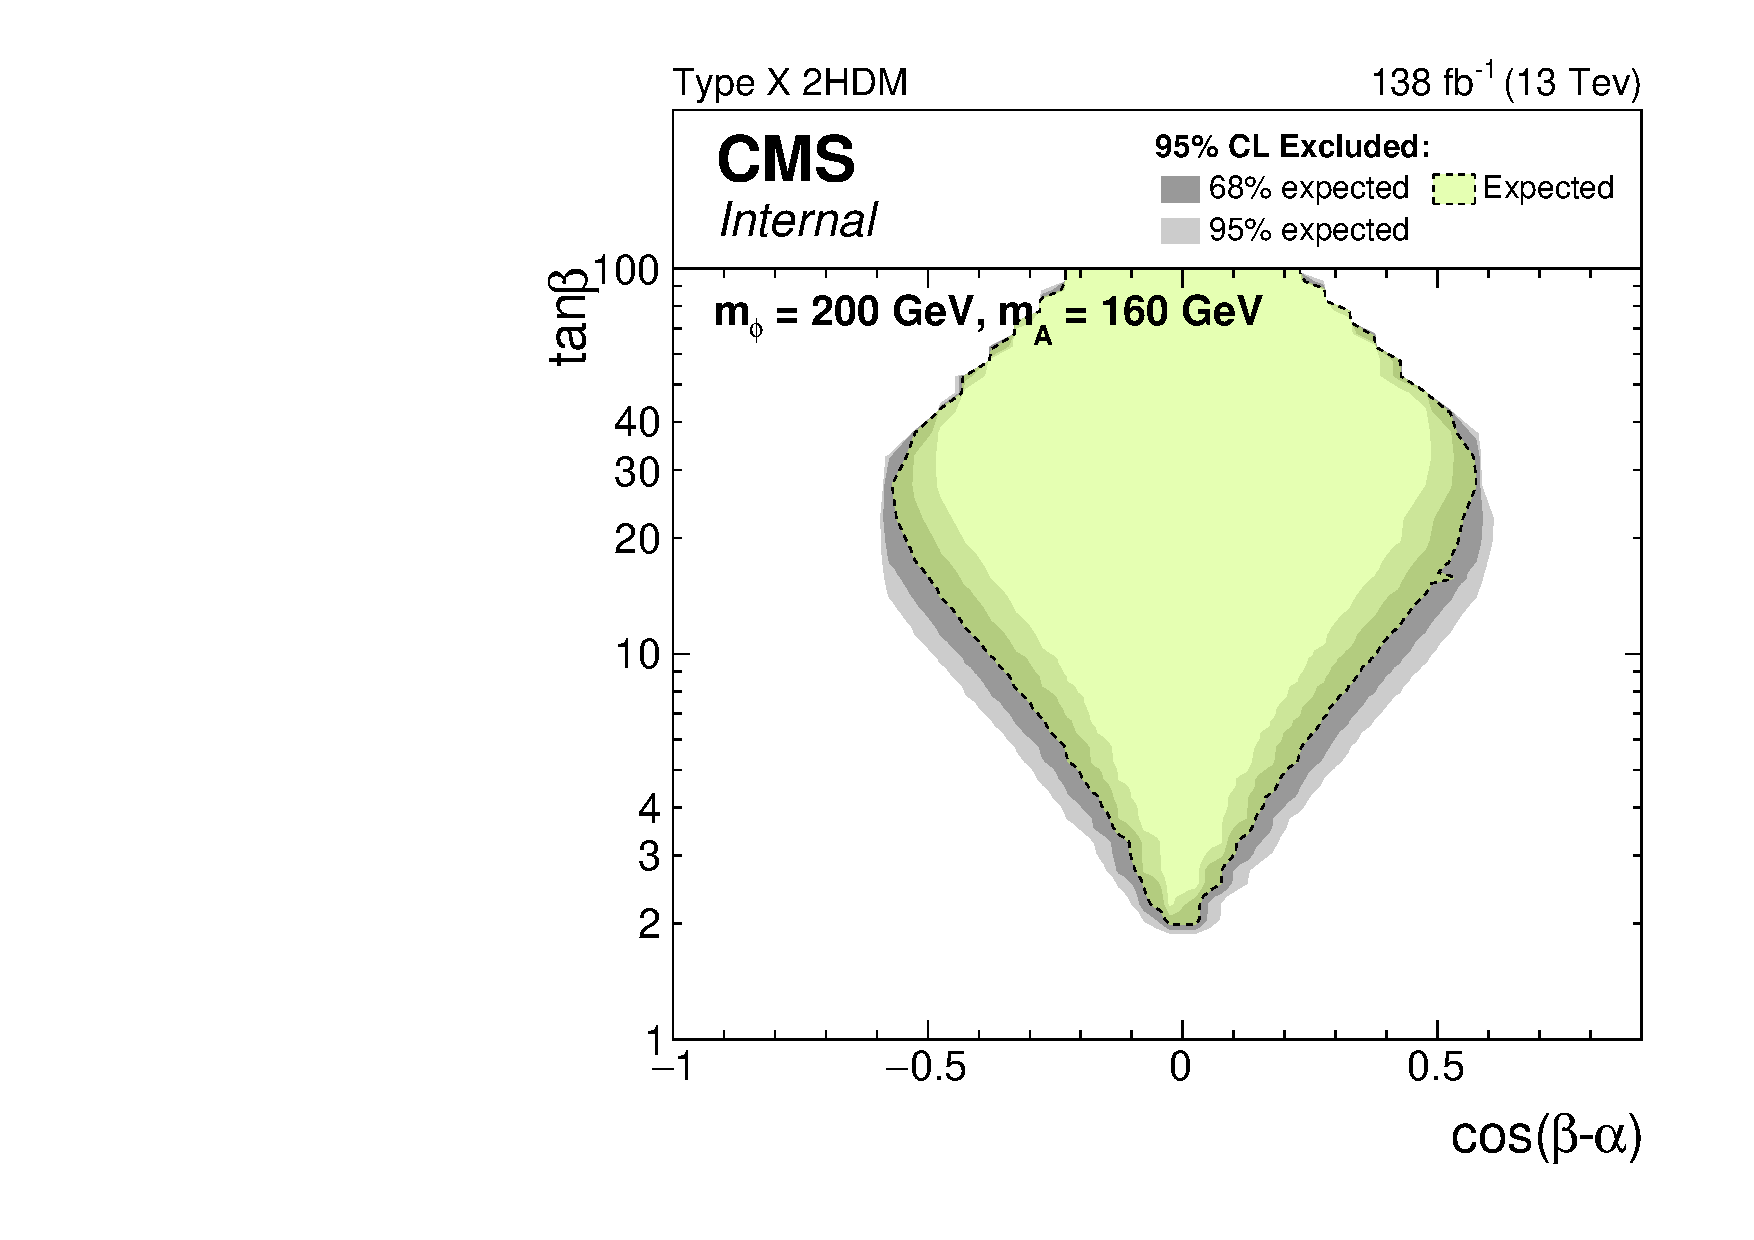
\includegraphics[width=0.65\textwidth]{Figures/csbma_phi200A160.pdf}} 
\caption{Expected and observed 95\% CL exclusion contours on the $\cos(\beta-\alpha)$-$\tan\beta$ phase space in the type X 2HDM alignment scenario with $m_{\phi}$ equal to 200 GeV and $m_{A}$ scenarios of 100 GeV (a) and 160 GeV (b). The exclusion limit only on background expectation is shown as a dashed black line, the dark and bright grey bands show the 68\% and 95\% intervals of the expected exclusion and the observed exclusion contour is shown by the blue area.}
\label{fig:4tau_cosbma}
\end{figure}